%%%%%%%%%%%%%%%%%%%%%%%%%%%%%%%%%%%%%%%%%%%%%%%%%%%%%%%%%%%%%%%%%%%%%%%%%
%  cSpell:disable
%  Zawartość: Główny plik szablonu pracy dyplomowej (magisterskiej/inżynierskiej). 
%  Opracował: Tomasz Kubik <tomasz.kubik@pwr.edu.pl>
%  Data: 9 lutego 2021
%  Wersja: 0.6
%  Wymagania: dedykowany do kompilatora pdflatex.
%%%%%%%%%%%%%%%%%%%%%%%%%%%%%%%%%%%%%%%%%%%%%%%%%%%%%%%%%%%%%%%%%%%%%%%%%

\documentclass[a4paper,onecolumn,oneside,12pt,extrafontsizes]{memoir}
%  W celu przygotowania wydruku  do archiwum można:
%  a) przygotować pdf, w którym dwie strony zostaną wstawione na jedną fizyczną stronę i taki dokument wydrukować dwustronnie (podejście zalecane)
%
%   Taki dokument można przygotować poprzez
%   - wydruk z Adobe Acrobat Reader z opcją "Wiele" - sekcja "Rozmiar i obsługa stron"
%   - wykorzystanie narzędzi psutils
%
%      Windows (zakładając, że w dystrybucji MiKTeX jest pakiet miktex-psutils-bin-x64-2.9):
%        "c:\Program Files\MiKTeX 2.9\miktex\bin\x64\pdf2ps.exe" Dyplom.pdf Dyplom.ps
%        "c:\Program Files\MiKTeX 2.9\miktex\bin\x64\psnup.exe" -2 Dyplom.ps Dyplom2.ps
%        "c:\Program Files\MiKTeX 2.9\miktex\bin\x64\ps2pdf.exe" Dyplom2.ps Dyplom2.pdf
%        Del Dyplom2.ps Dyplom.ps
%
%     Linux:
%        pdf2ps Dyplom.pdf - | psnup -2 | ps2pdf - Dyplom2.pdf
%
%  b) przekomplilować dokument zmniejszając czcionkę (podejście niezalecane, bo zmienia formatowanie dokumentu)
%
%    Do tego wystarczy posłużyć się poniższymi komendami (zamiast documentclass z pierwszej linijki):
%   \documentclass[a4paper,onecolumn,twoside,10pt]{memoir} 
%   \renewcommand{\normalsize}{\fontsize{8pt}{10pt}\selectfont}

% \usepackage[cp1250]{inputenc} % Proszę zostawić, jeśli kodowanie edytowanych plików to cp1250 
\usepackage[utf8]{inputenc} % Proszę użyć zamiast powyższego, jeśli kodowanie edytowanych plików to UTF8
\usepackage[T1]{fontenc}
\usepackage[english,polish]{babel} % Tutaj ważna jest kolejność atrybutów (dla pracy po polsku polish powinno być na końcu)
%\DisemulatePackage{setspace}
\usepackage{setspace}
\usepackage{color,calc}
%\usepackage{soul} % pakiet z komendami do podkreślania, przekreślania, podświetlania tekstu (raczej niepotrzebny)

\usepackage{ebgaramond} % pakiet z czcionkami garamond, potrzebny tylko do strony tytułowej, musi wystąpić przed pakietem tgtermes

%% Aby uzyskać polskie literki w pdfie (a nie zlepki) korzystamy z pakietu czcionek tgterms. 
%% W pakiecie tym są zdefiniowane klony czcionek Times o kształtach: normalny, pogrubiony, italic, italic pogrubiony.
%% W pakiecie tym brakuje czcionki o kształcie: slanted (podobny do italic). 
%% Jeśli w dokumencie gdzieś zostanie zastosowana czcionka slanted (np. po użyciu komendy \textsl{}), to
%% latex dokona podstawienia na czcionkę standardową i zgłosi to w ostrzeżeniu (warningu).
%% Ponadto tgtermes to czcionka do tekstu. Wszelkie matematyczne wzory będą sformatowane domyślną czcionką do wzorów.
%% Jeśli wzory mają być sformatowane z wykorzystaniem innych czcionek, trzeba to jawnie zadeklarować.

%% Po zainstalowaniu pakietu tgtermes może będzie trzeba zauktualizować informacje 
%% o dostępnych fontach oraz mapy. Można to zrobić z konsoli (jako administrator)
%% initexmf --admin --update-fndb
%% initexmf --admin --mkmaps

\usepackage{tgtermes}   
\renewcommand*\ttdefault{txtt}



\usepackage{multicol} % pakiet umożliwiający stworzenie wielokolumnowego tekstu
%%%%%%%%%%%%%%%%%%%%%%%%%%%%%%%%%%%%%%%%%%%%%%%%%%%
%% Pakiety do formatowania tabel
%%%%%%%%%%%%%%%%%%%%%%%%%%%%%%%%%%%%%%%%%%%%%%%%%%%
\usepackage{tabularx}
% Proszę używać tylko tabularx. Innych pakietów proszę nie stosować !!!
% Dokument na pewno da się zredagować bez ich użycia.
%\usepackage{longtable}
%\usepackage{ltxtable}
%\usepackage{tabulary}

%%%%%%%%%%%%%%%%%%%%%%%%%%%%%%%%%%%%%%%%%%%%%%%%%%%
%% Pakiet do wstawiania fragmentów kodu
%%%%%%%%%%%%%%%%%%%%%%%%%%%%%%%%%%%%%%%%%%%%%%%%%%%
\usepackage{listings} 
\usepackage{xpatch}
\makeatletter
\xpatchcmd\l@lstlisting{1.5em}{0em}{}{}
\makeatother
% Pakiet dostarcza otoczenia lstlisting. Jest ono wysoce konfigurowalne. 
% Konfigurować można indywidualnie każdy z listingów lub globalnie, w poleceniu \lstset{}.

% Zalecane jest, by kod źródłowy był wyprowadzany z użyciem czcionki maszynowej \ttfamily
% Ponieważ kod źródłowy, nawet po obcięciu do interesujących fragmentów, bywa obszerny, należy zmniejszyć czcionkę.
% Zalecane jest \small (dla krótkich fragmentów) oraz \footnotesize (dla dłuższych fragmentów).

% Ponadto podczas konfiguracji można zadeklarować sposób numerowania linii. Numerowanie linii zalecane jest jednak 
% tylko w przypadkach, gdy w opisie zamieszczonym w tekście znajdują się jakieś odwołania do konkretnych linii.
% Jeśli w opisie nie ma takich odwołań, numerowanie linii jest zbędne. Proszę wtedy go nie stosować.
% Przy włączaniu numerowania linii należy zwrócić uwagę na to, gdzie pojawią się te numery.
% Bez zmiany dodatkowych parametrów pojawiają się one na marginesie strony (co jest nieporządane).

\lstset{
  basicstyle=\small\ttfamily, % lub basicstyle=\footnotesize\ttfamily
  %%columns=fullflexible,
	%%showstringspaces=false,
	%%showspaces=false,
  breaklines=true,
  postbreak=\mbox{\textcolor{red}{$\hookrightarrow$}\space}, 
  %%numbers=left,  % ta i poniższe linie dotyczą ustawienia numerowania i sposobu jego wyprowadzania
  %%firstnumber=1, 
  %%numberfirstline=true, 
	%%xleftmargin=17pt,
  %%framexleftmargin=17pt,
  %%framexrightmargin=5pt,
  %%framexbottommargin=4pt,
	belowskip=.5\baselineskip
}

% Jeśli edytowany plik nie jest w kodowaniu cp1250, to jest problem z polskimi znakami występującymi we wstawianym kodzie.
% Dlatego podczas pracy na plikach w kodowaniu UTF-8 trzeba zadeklarować mapowanie jak niżej (wystarczy odmarkować).
% Niestety, jak się zastosuje to mapowanie mogą pojawić się problemy z podświetlaniem składni (patrz dalej).
\lstset{literate=%-
{ą}{{\k{a}}}1 {ć}{{\'c}}1 {ę}{{\k{e}}}1 {ł}{{\l{}}}1 {ń}{{\'n}}1 {ó}{{\'o}}1 {ś}{{\'s}}1 {ż}{{\.z}}1 {ź}{{\'z}}1 {Ą}{{\k{A}}}1 {Ć}{{\'C}}1 {Ę}{{\k{E}}}1 {Ł}{{\L{}}}1 {Ń}{{\'N}}1 {Ó}{{\'O}}1 {Ś}{{\'S}}1 {Ż}{{\.Z}}1 {Ź}{{\'Z}}1 
    {Ö}{{\"O}}1
    {Ä}{{\"A}}1
    {Ü}{{\"U}}1
    {ß}{{\ss}}1
    {ü}{{\"u}}1
    {ä}{{\"a}}1
    {ö}{{\"o}}1
    {~}{{\textasciitilde}}1
		{—}{{{\textemdash} }}1
}%{\ \ }{{\ }}1}


%% lstlisting pozwala na ostylowania podświetlania składni wybranych języków.
%% Działa to na zasadzie zdefiniowania słów kluczowych oraz sposobu ich wyświetlania.
%% Ponieważ jest to prosty mechanizm, czasem trudno osiągnąć takie efekty, jakie dają narzędzia IDE. 
%% Jednak w większości przypadku osiągane rezutlaty są zadowalające.
%%\lstloadlanguages{% Check Dokumentation for further languages ...
%%C,
%%C++,
%%csh,
%%Java
%%}


%% lstlisting obsługuje domyślnie kilka najpopularniejszych języków.
%% Inne języki muszą być dodefiniowane. Poniżej podano przykłady definicji języków i styli.

\definecolor{lightgray}{rgb}{.9,.9,.9}
\definecolor{darkgray}{rgb}{.4,.4,.4}
\definecolor{purple}{rgb}{0.65, 0.12, 0.82}
\definecolor{javared}{rgb}{0.6,0,0} % for strings
\definecolor{javagreen}{rgb}{0.25,0.5,0.35} % comments
\definecolor{javapurple}{rgb}{0.5,0,0.35} % keywords
\definecolor{javadocblue}{rgb}{0.25,0.35,0.75} % javadoc
 
\lstdefinelanguage{JavaScript}{ 
	keywords={typeof, new, true, false, catch, function, return, null, catch, switch, var, if, in, while, do, else, case, break},
	keywordstyle=\color{blue}\bfseries,
	ndkeywords={class, export, boolean, throw, implements, import, this},
	ndkeywordstyle=\color{darkgray}\bfseries,
	identifierstyle=\color{black},
	sensitive=false,
	comment=[l]{//},
	morecomment=[s]{/*}{*/},
	commentstyle=\color{purple}\ttfamily,
	stringstyle=\color{red}\ttfamily,
	morestring=[b]',
	morestring=[b]"
}
\lstdefinestyle{JavaScriptStyle}{
	language=JavaScript,
	commentstyle=\color{javagreen}, % niestety, jeśli w linii komentarza pojawią się słowa kluczowe, to zostaną pokolorowane
	backgroundcolor=,%\color{lightgray}, % można ustwić kolor tła, ale jest to niezalecane
	extendedchars=true,
	basicstyle=\footnotesize\ttfamily,
	showstringspaces=false,
	showspaces=false,
	numbers=none,%left,
	numberstyle=\footnotesize,
	numbersep=9pt,
	tabsize=2,
	breaklines=true,
	showtabs=false,
	captionpos=t
}

\lstdefinestyle{JavaStyle}{
basicstyle=\footnotesize\ttfamily,
keywordstyle=\color{javapurple}\bfseries,
stringstyle=\color{javared},
commentstyle=\color{javagreen},
morecomment=[s][\color{javadocblue}]{/**}{*/},
numbers=none,%left,
numberstyle=\tiny\color{black},
stepnumber=2,
numbersep=10pt,
tabsize=4,
showspaces=false,
showstringspaces=false,
captionpos=t
}

\definecolor{pblue}{rgb}{0.13,0.13,1}
\definecolor{pgreen}{rgb}{0,0.5,0}
\definecolor{pred}{rgb}{0.9,0,0}
\definecolor{pgrey}{rgb}{0.46,0.45,0.48}
\definecolor{dark-grey}{rgb}{0.4,0.4,0.4}
% styl json
\newcommand\JSONnumbervaluestyle{\color{blue}}
\newcommand\JSONstringvaluestyle{\color{red}}

\newif\ifcolonfoundonthisline

\makeatletter

\lstdefinestyle{json-style}  
{
	showstringspaces    = false,
	keywords            = {false,true},
	alsoletter          = 0123456789.,
	morestring          = [s]{"}{"},
	stringstyle         = \ifcolonfoundonthisline\JSONstringvaluestyle\fi,
	MoreSelectCharTable =%
	\lst@DefSaveDef{`:}\colon@json{\processColon@json},
	basicstyle          = \footnotesize\ttfamily,
	keywordstyle        = \ttfamily\bfseries,
	numbers				= left, % zamarkować, jeśli numeracja linii jest niepotrzebna
	numberstyle={\footnotesize\ttfamily\color{dark-grey}},
	xleftmargin			= 2em % zamarkować, jeśli numeracja linii jest niepotrzebna
}

\newcommand\processColon@json{%
	\colon@json%
	\ifnum\lst@mode=\lst@Pmode%
	\global\colonfoundonthislinetrue%
	\fi
}

\lst@AddToHook{Output}{%
	\ifcolonfoundonthisline%
	\ifnum\lst@mode=\lst@Pmode%
	\def\lst@thestyle{\JSONnumbervaluestyle}%
	\fi
	\fi
	\lsthk@DetectKeywords% 
}

\lst@AddToHook{EOL}%
{\global\colonfoundonthislinefalse}

\makeatother

%%\definecolor{red}{rgb}{0.6,0,0} % for strings
%%\definecolor{blue}{rgb}{0,0,0.6}
%%\definecolor{green}{rgb}{0,0.8,0}
%%\definecolor{cyan}{rgb}{0.0,0.6,0.6}
%%
%%\lstdefinestyle{sqlstyle}{
%%language=SQL,
%%basicstyle=\footnotesize\ttfamily, 
%%numbers=left, 
%%numberstyle=\tiny, 
%%numbersep=5pt, 
%%tabsize=2, 
%%extendedchars=true, 
%%breaklines=true, 
%%showspaces=false, 
%%showtabs=true, 
%%xleftmargin=17pt,
%%framexleftmargin=17pt,
%%framexrightmargin=5pt,
%%framexbottommargin=4pt,
%%keywordstyle=\color{blue}, 
%%commentstyle=\color{green}, 
%%stringstyle=\color{red}, 
%%}
%%
%%\lstdefinestyle{sharpcstyle}{
%%language=[Sharp]C,
%%basicstyle=\footnotesize\ttfamily, 
%%numbers=left, 
%%numberstyle=\tiny, 
%%numbersep=5pt, 
%%tabsize=2, 
%%extendedchars=true, 
%%breaklines=true, 
%%showspaces=false, 
%%showtabs=true, 
%%xleftmargin=17pt,
%%framexleftmargin=17pt,
%%framexrightmargin=5pt,
%%framexbottommargin=4pt,
%%morecomment=[l]{//}, %use comment-line-style!
%%morecomment=[s]{/*}{*/}, %for multiline comments
%%showstringspaces=false, 
%%morekeywords={  abstract, event, new, struct,
                %%as, explicit, null, switch,
                %%base, extern, object, this,
                %%bool, false, operator, throw,
                %%break, finally, out, true,
                %%byte, fixed, override, try,
                %%case, float, params, typeof,
                %%catch, for, private, uint,
                %%char, foreach, protected, ulong,
                %%checked, goto, public, unchecked,
                %%class, if, readonly, unsafe,
                %%const, implicit, ref, ushort,
                %%continue, in, return, using,
                %%decimal, int, sbyte, virtual,
                %%default, interface, sealed, volatile,
                %%delegate, internal, short, void,
                %%do, is, sizeof, while,
                %%double, lock, stackalloc,
                %%else, long, static,
                %%enum, namespace, string},
%%keywordstyle=\color{cyan},
%%identifierstyle=\color{red},
%%stringstyle=\color{blue}, 
%%commentstyle=\color{green},
%%}


% Przedefiniowanie komendy wstawiającej Spis listingów do dokumentu. 
%\renewcommand\lstlistlistingname{Spis listingów}
% Bez przedefiniowania nagłówek tego spisu pojawiał się na innej wysokości niż nagłówki innych spisów.
%%%\makeatletter
%%%%\renewcommand*{\l@lstlisting}[2]{\@dottedtocline{1}{0em}{2.3em}{#1}{#2}}
%%%\g@addto@macro\insertchapterspace{\addtocontents{lol}{\protect\addvspace{10pt}}}
%%%\renewcommand*{\l@lstlisting}{\@dottedtocline{1}{0em}{2.3em}}
%%%\makeatother


\makeatletter % odstępy w spisie pomiędzy rozdziałami
\renewcommand*{\insertchapterspace}{%
  \addtocontents{lof}{\protect\addvspace{5pt}}%
  \addtocontents{lot}{\protect\addvspace{5pt}}%
	\addtocontents{toc}{\protect\addvspace{5pt}} %
  \addtocontents{lol}{\protect\addvspace{5pt}}}
\makeatother 

\newcommand{\listingcaption}[1]% dodane, by można było robić podpis nad dwukolumnowym listingiem
{%
\vspace*{\abovecaptionskip}\small 
\refstepcounter{lstlisting}\hfill%
Listing \thelstlisting: #1\hfill%\hfill%
\addcontentsline{lol}{lstlisting}{\protect\numberline{\thelstlisting}#1}
}%

% Redefinitions of labels for tables, figures and bibliography 
%\AtBeginDocument{% 
        \addto\captionspolish{% 
        \renewcommand{\lstlistlistingname}{Spis listingów}%
}%} 
\newlistof{lstlistoflistings}{lol}{\lstlistlistingname}


%%%%%%%%%%%%%%%%%%%%%%%%%%%%%%%%%%%%%%%%%%%%%%%%%%%
%% Ustawienia odpowiedzialne za sposób łamania dokumentu
%% i ułożenie elementów pływających
%%%%%%%%%%%%%%%%%%%%%%%%%%%%%%%%%%%%%%%%%%%%%%%%%%%
%\hyphenpenalty=10000		% nie dziel wyrazów zbyt często
\clubpenalty=10000      %kara za sierotki
\widowpenalty=10000  % nie pozostawiaj wdów
%\brokenpenalty=10000		% nie dziel wyrazów między stronami - trzeba było wyłączyć, bo nie łamały się linie w lstlisting
%\exhyphenpenalty=999999		% nie dziel słów z myślnikiem - trzeba było wyłączyć, bo nie łamały się linie w lstlisting
\righthyphenmin=3			% dziel minimum 3 litery

%\tolerance=4500
%\pretolerance=250
%\hfuzz=1.5pt
%\hbadness=1450

\renewcommand{\topfraction}{0.95}
\renewcommand{\bottomfraction}{0.95}
\renewcommand{\textfraction}{0.05}
\renewcommand{\floatpagefraction}{0.35}

%%%%%%%%%%%%%%%%%%%%%%%%%%%%%%%%%%%%%%%%%%%%%%%%%%%
%%  Ustawienia rozmiarów: tekstu, nagłówka i stopki, marginesów
%%  dla dokumentów klasy memoir 
%%%%%%%%%%%%%%%%%%%%%%%%%%%%%%%%%%%%%%%%%%%%%%%%%%%
\setlength{\headsep}{10pt} 
\setlength{\headheight}{13.6pt} % wartość baselineskip dla czcionki 11pt tj. \small wynosi 13.6pt
\setlength{\footskip}{\headsep+\headheight}
\setlength{\uppermargin}{\headheight+\headsep+1cm}
\setlength{\textheight}{\paperheight-\uppermargin-\footskip-1.5cm}
\setlength{\textwidth}{\paperwidth-5cm}
\setlength{\spinemargin}{2.5cm}
\setlength{\foremargin}{2.5cm}
\setlength{\marginparsep}{2mm}
\setlength{\marginparwidth}{2.3mm}
%\settrimmedsize{297mm}{210mm}{*}
%\settrims{0mm}{0mm}	
\checkandfixthelayout[fixed] % konieczne, aby się dobrze wszystko poustawiało
%%%%%%%%%%%%%%%%%%%%%%%%%%%%%%%%%%%%%%%%%%%%%%%%
%%  Ustawienia odległości linii, wcięć, odstępów
%%%%%%%%%%%%%%%%%%%%%%%%%%%%%%%%%%%%%%%%%%%%%%%%
\linespread{1}
%\linespread{1.241}
\setlength{\parindent}{14.5pt}

\setlength{\cftbeforechapterskip}{0pt} % odstępy w spisie treści przed rozdziałem, działa w korelacji z:
\renewcommand{\aftertoctitle}{\afterchaptertitle\vspace{-4pt}} % co trzeba zmienić, by tekst w spisie treści zaczynał się na tej samej wysokości co w innych spisach

%\cftsetindents{section}{1.5em}{2.3em}

%\setbeforesecskip{10pt plus 0.5ex}%{-3.5ex \@plus -1ex \@minus -.2ex}
%\setaftersecskip{10pt plus 0.5ex}%\onelineskip}
%\setbeforesubsecskip{8pt plus 0.5ex}%{-3.5ex \@plus -1ex \@minus -.2ex}
%\setaftersubsecskip{8pt plus 0.5ex}%\onelineskip}
%\setlength\floatsep{6pt plus 2pt minus 2pt} 
%\setlength\intextsep{12pt plus 2pt minus 2pt} 
%\setlength\textfloatsep{12pt plus 2pt minus 2pt} 

%%%%%%%%%%%%%%%%%%%%%%%%%%%%%%%%%%%%%%%%%%%%%%%%%%%
%%  Pakiety i komendy zastosowane tylko do zamieszczenia informacji o użytych komendach i fontach w tym szablonie.
%%  Normalnie nie są one potrzebne. Proszę poniższe deklaracje zamarkować podczas redakcji pracy !!!!
%%%%%%%%%%%%%%%%%%%%%%%%%%%%%%%%%%%%%%%%%%%%%%%%%%%
\usepackage{memlays}     % extra layout diagrams, zastosowane w szblonie do 'debuggowania', używa pakietu layouts
%\usepackage{layouts}
\usepackage{printlen} % pakiet do wyświetlania wartości zdefiniowanych długości, stosowany do 'debuggowania'
\uselengthunit{pt}
\makeatletter
\newcommand{\showFontSize}{\f@size pt} % makro wypisujące wielkość bieżącej czcionki
\makeatother
% do pokazania ramek można byłoby użyć:
%\usepackage{showframe} 


%%%%%%%%%%%%%%%%%%%%%%%%%%%%%%%%%%%%%%%%%%%%%%%%%%%
%%  Formatowanie list wyliczeniowych, wypunktowań i własnych otoczeń
%%%%%%%%%%%%%%%%%%%%%%%%%%%%%%%%%%%%%%%%%%%%%%%%%%%

% Domyślnie wypunktowania mają zadeklatorowane znaki, które nie występują w tgtermes
% Aby latex nie podstawiał w ich miejsca znaków z czcionki standardowej można zrobić podstawienie:
%    \DeclareTextCommandDefault{\textbullet}{\ensuremath{\bullet}}
%    \DeclareTextCommandDefault{\textasteriskcentered}{\ensuremath{\ast}}
%    \DeclareTextCommandDefault{\textperiodcentered}{\ensuremath{\cdot}}
% Jednak jeszcze lepszym pomysłem jest zdefiniowanie otoczeń z wykorzystaniem enumitem
\usepackage{enumitem} % pakiet pozwalający zarządzać formatowaniem list wyliczeniowych
\setlist{noitemsep,topsep=4pt,parsep=0pt,partopsep=4pt,leftmargin=*} % zadeklarowane parametry pozwalają uzyskać 'zwartą' postać wypunktowania bądź wyliczenia
\setenumerate{labelindent=0pt,itemindent=0pt,leftmargin=!,label=\arabic*.} % można zmienić \arabic na \alph, jeśli wyliczenia mają być z literkami
\setlistdepth{4} % definiujemy głębokość zagnieżdżenia list wyliczeniowych do 4 poziomów
\setlist[itemize,1]{label=$\bullet$}  % definiujemy, jaki symbol ma być użyty w wyliczeniu na danym poziomie
\setlist[itemize,2]{label=\normalfont\bfseries\textendash}
\setlist[itemize,3]{label=$\ast$}
\setlist[itemize,4]{label=$\cdot$}
\renewlist{itemize}{itemize}{4}

%%%http://tex.stackexchange.com/questions/29322/how-to-make-enumerate-items-align-at-left-margin
%\renewenvironment{enumerate}
%{
%\begin{list}{\arabic{enumi}.}
%{
%\usecounter{enumi}
%%\setlength{\itemindent}{0pt}
%%\setlength{\leftmargin}{1.8em}%{2zw} % 
%%\setlength{\rightmargin}{0zw} %
%%\setlength{\labelsep}{1zw} %
%%\setlength{\labelwidth}{3zw} % 
%\setlength{\topsep}{6pt}%
%\setlength{\partopsep}{0pt}%
%\setlength{\parskip}{0pt}%
%\setlength{\parsep}{0em} % 
%\setlength{\itemsep}{0em} % 
%%\setlength{\listparindent}{1zw} % 
%}
%}{
%\end{list}
%}

\makeatletter
\renewenvironment{quote}{
	\begin{list}{}
	{
	\setlength{\leftmargin}{1em}
	\setlength{\topsep}{0pt}%
	\setlength{\partopsep}{0pt}%
	\setlength{\parskip}{0pt}%
	\setlength{\parsep}{0pt}%
	\setlength{\itemsep}{0pt}
	}
	}{
	\end{list}}
\makeatother

%%%%%%%%%%%%%%%%%%%%%%%%%%%%%%%%%%%%%%%%%
%%  Pakiet i komendy do generowania indeksu 
%% (ważne, by pojawiły się przed pakietem hyperref)
%%%%%%%%%%%%%%%%%%%%%%%%%%%%%%%%%%%%%%%%%
% pdftex jest w stanie wygenerować indeks (czyli spis haseł z referencjami do stron, na których te hasła się pojawiły).
% Generalnie z indeksem jest sporo problemów, zwłaszcza, gdy pojawiają się polskie literki.
% Trzeba wtedy korzystać z xindy.
% Zwykle w pracach dyplomowych indeksy nie są wykorzystywane. Dlatego są zamarkowane.
%\DisemulatePackage{imakeidx}
%\usepackage[makeindex,noautomatic]{imakeidx} % tutaj mówimy, żeby indeks nie generował się automatycznie, 
%\makeindex
%
%\makeatletter
%%%%\renewenvironment{theindex}
							 %%%%{\vskip 10pt\@makeschapterhead{\indexname}\vskip -3pt%
								%%%%\@mkboth{\MakeUppercase\indexname}%
												%%%%{\MakeUppercase\indexname}%
								%%%%\vspace{-3.2mm}\parindent\z@%
								%%%%\renewcommand\subitem{\par\hangindent 16\p@ \hspace*{0\p@}}%%
								%%%%\phantomsection%
								%%%%\begin{multicols}{2}
								%%%%%\thispagestyle{plain}
								%%%%\parindent\z@                
								%%%%%\parskip\z@ \@plus .3\p@\relax
								%%%%\let\item\@idxitem}
							 %%%%{\end{multicols}\clearpage}
%%%%
%\makeatother



%%%%%%%%%%%%%%%%%%%%%%%%%%%%%%%%%%%%%%%%%
%%  Sprawy metadanych w wynikowym pdf, hyperlinków itp.
%%%%%%%%%%%%%%%%%%%%%%%%%%%%%%%%%%%%%%%%%
% Szablon przygotowano głównie dla pdflatex. Specyficzne komendy dla pdf-owej kompilacj wstawiono 
% w instrukcję warunkową dostarczaną przez pakiet ifpdf 
\usepackage{ifpdf}
%\newif\ifpdf \ifx\pdfoutput\undefined
%\pdffalse % we are not running PDFLaTeX
%\else
%\pdfoutput=1 % we are running PDFLaTeX
%\pdftrue \fi
\ifpdf
 \usepackage{datetime} % INFO: pakiet potrzeby do uzyskania i sformatowania daty 
 \usepackage[pdftex,bookmarks,breaklinks,unicode]{hyperref}
 \usepackage[pdftex]{graphicx}
 \DeclareGraphicsExtensions{.pdf,.jpg,.mps,.png} % po zadeklarowaniu rozszerzeń można będzie wstawiać pliki z grafiką bez konieczności podawania tych rozszerzeń w ich nazwach
\pdfcompresslevel=9
\pdfoutput=1

% Dobrze przygotowany dokument pdf to taki, który zawiera metadane.
% Poniżej zadeklarowano pola metadanych, jakie będą włączone do dokumentu pdf.
% Należy je odpowiednio uzupełnić (domyślnie wstawiany jest tytuł, autor, data modyfikacji)
\makeatletter
\AtBeginDocument{  
  \hypersetup{
	pdfinfo={
    Title = {\@title},
    Author = {\@author},
    Subject={},  
    Keywords={raz, dwa, trzy, cztery}, 
		Producer={}, 
	  CreationDate= {}, % zgodnie ze składnią: {D:yyyymmddhhmmss}, np. D:20210208175600
    ModDate={D:\pdfdate},   % data modyfikacji będzie datą kompilacji
		Creator={pdftex},
	}}
}
\pdftrailerid{} %Remove ID
\pdfsuppressptexinfo15 %Suppress PTEX.Fullbanner and info of imported PDFs

\makeatother
\else             % jeśli kompilacja jest inna niż pdflatex
\usepackage{graphicx}
\DeclareGraphicsExtensions{.eps,.ps,.jpg,.mps,.png}
\fi
\sloppy

\def\UrlBreaks{\do\/\do-\do_} % dodane by lepiej łamać urle 

%\graphicspath{{rys01/}{rys02/}}  % choć można zadeklarować foldery, w jakich pojawiać się mają pliki z grafiką, zaleca się jednak, by tego nie robić


%%%%%%%%%%%%%%%%%%%%%%%%%%%%%%%%%%%%%%%%%
%%  Formatowanie dokumentu
%%%%%%%%%%%%%%%%%%%%%%%%%%%%%%%%%%%%%%%%%
% INFO: Deklaracja głębokościu numeracji
\setcounter{secnumdepth}{2}
\setcounter{tocdepth}{2}
\setsecnumdepth{subsection} 
% INFO: Dodanie kropek po numerach sekcji
\makeatletter
\def\@seccntformat#1{\csname the#1\endcsname.\quad}
\def\numberline#1{\hb@xt@\@tempdima{#1\if&#1&\else.\fi\hfil}}
\makeatother
% INFO: Numeracja rozdziałów i separatory
\renewcommand{\chapternumberline}[1]{#1.\quad}
\renewcommand{\cftchapterdotsep}{\cftdotsep}

% Czcionka do podpisów tabel i rysunków
\captionnamefont{\small}
\captiontitlefont{\small}
% INFO: Makro pozwalające zmienić sposób wypisywania rozdziału (proszę z niego nie korzystać)
%\def\printchaptertitle##1{\fonttitle \space \thechapter.\space ##1} 

% Przedefiniowanie etykiet w podpisach tabel i rysunków
%\AtBeginDocument{% 
        \addto\captionspolish{% 
        \renewcommand{\tablename}{Tab.}% 
}%} 

%\AtBeginDocument{% 
%        \addto\captionspolish{% 
%        \renewcommand{\chaptername}{Rozdział}% 
%}} 

%\AtBeginDocument{% 
        \addto\captionspolish{% 
        \renewcommand{\figurename}{Rys.}% 
}%}


%\AtBeginDocument{% 
        \addto\captionspolish{% 
        \renewcommand{\bibname}{Literatura}% 
}%}

%\AtBeginDocument{% 
        \addto\captionspolish{% 
        \renewcommand{\listfigurename}{Spis rysunków}% 
}%}

%\AtBeginDocument{% 
        \addto\captionspolish{% 
        \renewcommand{\listtablename}{Spis tabel}% 
}%}

%\AtBeginDocument{% 
        \addto\captionspolish

%\AtBeginDocument{% 
    \addto\captionspolish{
\renewcommand\abstractname{Streszczenie} % niepotrzebne, bo przy polskich ustawieniach językowych jest 'Streszczenie'
}%}

%\AtBeginDocument{% 
    \addto\captionsenglish{
\renewcommand\abstractname{Abstract} % niepotrzebne, bo przy polskich ustawieniach językowych jest 'Streszczenie'
}%}

\renewcommand{\abstractnamefont}{\normalfont\Large\bfseries}
\renewcommand{\abstracttextfont}{\normalfont}

\newcommand\mykeywords[1]{\hspace{\absleftindent}\parbox{\linewidth-2.0\absleftindent}{
       \iflanguage{polish}{\textbf{Słowa kluczowe:} #1}{%
			  \iflanguage{english}{\textbf{Keywords:} #1}}{}}
				}

%%%%%%%%%%%%%%%%%%%%%%%%%%%%%%%%%%%%%%%%%%%%%%%%%%%%%%%%%%%%%%%%%%                  
%% Definicje stopek i nagłówków
%%%%%%%%%%%%%%%%%%%%%%%%%%%%%%%%%%%%%%%%%%%%%%%%%%%%%%%%%%%%%%%%%%                  
\addtopsmarks{headings}{%
\nouppercaseheads % added at the beginning
}{%
\createmark{chapter}{both}{shownumber}{}{. \space}
%\createmark{chapter}{left}{shownumber}{}{. \space}
\createmark{section}{right}{shownumber}{}{. \space}
}%use the new settings

\makeatletter
\copypagestyle{outer}{headings}
\makeoddhead{outer}{}{}{\small\itshape\rightmark}
\makeevenhead{outer}{\small\itshape\leftmark}{}{}
\makeoddfoot{outer}{\small\@author:~\@titleShort}{}{\small\thepage}
\makeevenfoot{outer}{\small\thepage}{}{\small\@author:~\@title}
\makeheadrule{outer}{\linewidth}{\normalrulethickness}
\makefootrule{outer}{\linewidth}{\normalrulethickness}{2pt}
\makeatother

% fix plain
\copypagestyle{plain}{headings} % overwrite plain with outer
\makeoddhead{plain}{}{}{} % remove right header
\makeevenhead{plain}{}{}{} % remove left header
\makeevenfoot{plain}{}{}{}
\makeoddfoot{plain}{}{}{}

\copypagestyle{empty}{headings} % overwrite plain with outer
\makeoddhead{empty}{}{}{} % remove right header
\makeevenhead{empty}{}{}{} % remove left header
\makeevenfoot{empty}{}{}{}
\makeoddfoot{empty}{}{}{}


%%%%%%%%%%%%%%%%%%%%%%%%%%%%%%%%%%%%%%%
%% Definicja strony tytułowej 
%%%%%%%%%%%%%%%%%%%%%%%%%%%%%%%%%%%%%%%
\makeatletter
%Uczelnia
\newcommand\uczelnia[1]{\renewcommand\@uczelnia{#1}}
\newcommand\@uczelnia{}
%Wydział
\newcommand\wydzial[1]{\renewcommand\@wydzial{#1}}
\newcommand\@wydzial{}
%Kierunek
\newcommand\kierunek[1]{\renewcommand\@kierunek{#1}}
\newcommand\@kierunek{}
%Specjalność
\newcommand\specjalnosc[1]{\renewcommand\@specjalnosc{#1}}
\newcommand\@specjalnosc{}
%Tytuł po angielsku
\newcommand\titleEN[1]{\renewcommand\@titleEN{#1}}
\newcommand\@titleEN{}
%Tytuł krótki
\newcommand\titleShort[1]{\renewcommand\@titleShort{#1}}
\newcommand\@titleShort{}
%Promotor
\newcommand\promotor[1]{\renewcommand\@promotor{#1}}
\newcommand\@promotor{}

\def\maketitle{%
  \pagestyle{empty}%
%%\garamond 
	\fontfamily{\ebgaramond@family}\selectfont % na stronie tytułowej czcionka garamond
%%%%%%%%%%%%%%%%%%%%%%%%%%%%%%%%%%%%%	
%% Poniżej, w otoczniu picture, wstawiono tytuł i autora. 
%% Tytuł (z autorem) musi znaleźć się w obszarze 
%% odpowiadającym okienku 110mmx75mm, którego lewy górny róg 
%% jest w położeniu 77mm od lewej i 111mm od górnej  krawędzi strony 
%% (tak wynika z wycięcia na okładce). 
%% Poniższy kod musi być użyty dokładnie w miejscu gdzie jest.
%% Jeśli tytuł nie mieści się w okienku, to należy tak pozmieniać 
%% parametry użytych komend, aby ten przydługi tytuł jednak 
%% upakować go do okienka.
%%
%% Sama okładka (kolorowa strona z wycięciem, do pobrania z dydaktyki) 
%% powinna być przycięta o 3mm od każdej z krawędzi.
%% Te 3mm pewnie zostawiono na ewentualne spady czy też specjalną oprawę.
%%%%%%%%%%%%%%%%%%%%%%%%%%%%%%%%%%%%%	
\newlength{\tmpfboxrule}
\setlength{\tmpfboxrule}{\fboxrule}
\setlength{\fboxsep}{2mm}
\setlength{\fboxrule}{0mm} 
%\setlength{\fboxrule}{0.1mm} %% INFO: Jeśli chcemy zobaczyć ramkę, wystarczy odmarkować tę linijkę
\setlength{\unitlength}{1mm}
\begin{picture}(0,0)
\put(26,-124){\fbox{
\parbox[c][71mm][c]{104mm}{\centering%\lineskip=34pt 
\fontsize{16pt}{18pt}\selectfont \@title\\[5mm]
\fontsize{16pt}{18pt}\selectfont \@titleEN\\[20mm]
\fontsize{16pt}{18pt}\selectfont AUTOR:\\[2mm]
\fontsize{14pt}{16pt}\selectfont \@author}
}
}
\end{picture}
\setlength{\fboxrule}{\tmpfboxrule} 
%%%%%%%%%%%%%%%%%%%%%%%%%%%%%%%%%%%%%
%% Reszta strony z nazwą uczelni, wydziału, kierunkiem, specjalnością
%% promotorem, oceną pracy, miastem i rokiem
	{\centering%\vspace{-1cm}
		{\fontsize{22pt}{24pt}\selectfont \@uczelnia}\\[0.4cm]
		{\fontsize{22pt}{24pt}\selectfont \@wydzial}\\[0.5cm]
		  \hrule %\vspace*{0.7cm}
	}
{\flushleft\fontsize{14pt}{16pt}\selectfont%
\begin{tabular}{ll}
KIERUNEK: & \@kierunek\\
SPECJALNOŚĆ: & \@specjalnosc\\
\end{tabular}\\[1.3cm]
}
{\centering
{\fontsize{32pt}{36pt}\selectfont PRACA DYPLOMOWA}\\[0.5cm]
{\fontsize{32pt}{36pt}\selectfont MAGISTERSKA}\\[2.5cm]
}
\vfill
\begin{tabularx}{\linewidth}{p{6cm}X}
		&{\fontsize{16pt}{18pt}\selectfont PROWADZĄCY PRACĘ:}\\[2mm] %INFO: tutaj jest miejsce na nazwisko promotora pracy
		&{\fontsize{14pt}{16pt}\selectfont \@promotor}\\[10mm]
%		&{\fontsize{16pt}{18pt}\selectfont OCENA PRACY:}\\[20mm]
% Tekst 'OCENA PRACY:' można usunąć, jeśli praca ma być dostarczona bez podpisu promotora (w dobie pandemii)
% Czyli zamiast powyżej zdefiniowanego wiersza tabeli można wpisać:
   &{\fontsize{16pt}{18pt}\selectfont }\\[20mm]
	\end{tabularx}
\vspace{2cm}
\hrule\vspace*{0.3cm}
{\centering
{\fontsize{16pt}{18pt}\selectfont \@date}\\[0cm]
}
%\ungaramond
\normalfont
 \cleardoublepage
}
\makeatother
%%%%%%%%%%%%%%%%%%%%%%%%%%%%%%%%%%%%%%%%%

%\AtBeginDocument{\addtocontents{toc}{\protect\thispagestyle{empty}}}


%%%%%%%%%%%%%%%%%%%%%%%%%%%%%%%%%%%%%%%%%
%%  Metadane dokumentu 
%%%%%%%%%%%%%%%%%%%%%%%%%%%%%%%%%%%%%%%%%
\title{Metoda automatycznej oceny podobieństwa semantycznego tekstów na potrzeby analizy dyskursu publicznego}
\titleShort{Metoda automatycznej oceny podobieństwa semantycznego tekstów \dots}
\titleEN{Automatic assessment of semantic similarity of texts for the analysis of public discourse}
\author{Marcin Kotas}
\uczelnia{POLITECHNIKA WROCŁAWSKA}
\wydzial{WYDZIAŁ ELEKTRONIKI}
\kierunek{INFORMATYKA (INF)}
\specjalnosc{GRAFIKA I SYSTEMY MULTIMEDIALNE (IGM)}
\promotor{dr inż. Tomasz Walkowiak W4/K9}
\date{WROCŁAW, 2021}

% Ustawienie odstępu od góry w nienumerowanych rozdziałach oraz wykazach:
% Spis treści, Spis tabel, Spis rysunków, Indeks rzeczowy

%\newlength{\linespace}
%\setlength{\linespace}{-\beforechapskip-\topskip+\headheight+\topsep}
%%%\makechapterstyle{noNumbered}{%
%%%\renewcommand\chapterheadstart{\vspace*{\linespace}}
%%%}

%% powyższa komenda załatwia to, co robią komendy poniższe dla spisów
%\renewcommand*{\tocheadstart}{\vspace*{\linespace}}
%\renewcommand*{\lotheadstart}{\vspace*{\linespace}}
%\renewcommand*{\lofheadstart}{\vspace*{\linespace}}

%%%%%%%%%%%%%%%%%%%%%%%%%%%%%%%%%%%%%%%%%
%                  Początek dokumentu 
%%%%%%%%%%%%%%%%%%%%%%%%%%%%%%%%%%%%%%%%%
% INFO: Za pomocą polecenia \includeonly{} można dokonać selekcji części składowych dokumentu (plików z latexowym kodem), jakie mają być kompilowane. 
%       Przydaje się to szczególnie podczas pracy nad dużymi dokumentami. 
%       Bo im mniej jest części składowych do przetworzenia, tym szybsza jest kompilacja.
%       Proszę nie mylić tej komendy z poleceniem \include{}, którą używa się do zadeklarowania części składowych dokumentu (plików z latexowym kodem).

%\includeonly{skroty,rozdzial01}  

\begin{document}
% Komendami poniżej można przełączyć odstęp między liniami. Proszę jednak tego nie robić !!!
%\SingleSpacing
%\OnehalfSpacing
%\DoubleSpacing

%\settypeoutlayoutunit{cm} % do debugowania
%\typeoutstandardlayout    % wypisuje na stdout informacje o ustawieniach

%\frontmatter
\pdfbookmark[0]{Tytuł}{Tytul.1}
\maketitle
\clearpage
%\chapterstyle{noNumbered}
\pagestyle{outer}
\pdfbookmark[0]{Streszczenie}{streszczenie.1}
%\phantomsection
%\addcontentsline{toc}{chapter}{Streszczenie}
%%% Poniższe zostało niewykorzystane (tj. zrezygnowano z utworzenia nienumerowanego rozdziału na abstrakt)
%%%\begingroup
%%%\setlength\beforechapskip{48pt} % z jakiegoś powodu była maleńka różnica w położeniu nagłówka rozdziału numerowanego i nienumerowanego
%%%\chapter*{\centering Abstrakt}
%%%\endgroup
%%%\label{sec:abstrakt}
%%%Lorem ipsum dolor sit amet eleifend et, congue arcu. Morbi tellus sit amet, massa. Vivamus est id risus. Sed sit amet, libero. Aenean ac ipsum. Mauris vel lectus. 
%%%
%%%Nam id nulla a adipiscing tortor, dictum ut, lobortis urna. Donec non dui. Cras tempus orci ipsum, molestie quis, lacinia varius nunc, rhoncus purus, consectetuer congue risus. 
%\mbox{}\vspace{2cm} % można przesunąć, w zależności od długości streszczenia
\begin{abstract}
Lorem ipsum dolor sit amet eleifend et, congue arcu. Morbi tellus sit amet, massa. Vivamus est id risus. Sed sit amet, libero. Aenean ac ipsum. Mauris vel lectus. 

Nam id nulla a adipiscing tortor, dictum ut, lobortis urna. Donec non dui. Cras tempus orci ipsum, molestie quis, lacinia varius nunc, rhoncus purus, consectetuer congue risus. 
\end{abstract}
\mykeywords{raz, dwa, trzy, cztery}\\ 
% Dobrze byłoby skopiować słowa kluczowe do metadanych dokumentu pdf (w pliku Dyplom.tex)
% Niestety, zaimplementowane makro nie robi tego z automatu, więc pozostaje kopiowanie ręczne.

{
\selectlanguage{english}
\begin{abstract}
Lorem ipsum dolor sit amet eleifend et, congue arcu. Morbi tellus sit amet, massa. Vivamus est id risus. Sed sit amet, libero. Aenean ac ipsum. Mauris vel lectus. 

Nam id nulla a adipiscing tortor, dictum ut, lobortis urna. Donec non dui. Cras tempus orci ipsum, molestie quis, lacinia varius nunc, rhoncus purus, consectetuer congue risus. 
\end{abstract}
\mykeywords{one, two, three, four}
}
 
\clearpage
\pdfbookmark[0]{Spis treści}{spisTresci.1}%
%%\phantomsection
%%\addcontentsline{toc}{chapter}{Spis treści}
\tableofcontents* 
\clearpage
\pdfbookmark[0]{Spis rysunków}{spisRysunkow.1} % jeśli chcemy mieć w spisie treści, to zamarkować tę linię, a odmarkować linie poniższe
%%\phantomsection
%%\addcontentsline{toc}{chapter}{Spis rysunków}
\listoffigures*
\clearpage
\pdfbookmark[0]{Spis tabel}{spisTabel.1} %
%%\phantomsection
%%\addcontentsline{toc}{chapter}{Spis tabel}
\listoftables*
\clearpage
\pdfbookmark[0]{Spis listingów}{spisListingow.1} %
%%\phantomsection
%%\addcontentsline{toc}{chapter}{Spis listingów}
\lstlistoflistings*
\clearpage
\pdfbookmark[0]{Skróty}{skroty.1}% 
%%\phantomsection
%%\addcontentsline{toc}{chapter}{Skróty}
\chapter*{Skróty}
\label{sec:skroty}
\noindent\vspace{-\topsep-\partopsep-\parsep} % Jeśli zaczyna się od otoczenia description, to otoczenie to ląduje lekko niżej niż wylądowałby zwykły tekst, dlatego wstawiano przesunięcie w pionie
\begin{description}[labelwidth=*]
  \item [OGC] (ang.\ \emph{Open Geospatial Consortium}) %-- jednostka arytmetyczno--logiczna
  \item [XML] (ang.\ \emph{eXtensible Markup Language})
  \item [SOAP] (ang.\ \emph{Simple Object Access Protocol})
  \item [WSDL] (ang.\ \emph{Web Services Description Language})
  \item [UDDI] (ang.\ \emph{Universal Description Discovery and Integration})
  \item [GIS] (ang.\ \emph{Geographical Information System})
  \item [SDI] (ang.\ \emph{Spatial Data Infrastructure})
  \item [ISO] (ang.\ \emph{International Standards Organization})
  \item [WMS] (ang.\ \emph{Web Map Service})
  \item [WFS] (ang.\ \emph{Web Feature Service})
  \item [WPS] (ang.\ \emph{Web Processing Service})
  \item [GML] (ang.\ \emph{Geography Markup Language})
  \item [SRG] (ang.\ \emph{Seeded Region Growing})
  \item [SOA] (ang.\ \emph{Service Oriented Architecture })
  \item [IT] (ang.\ \emph{Information Technology })
\end{description}
 %skróty można sobie pominąć


%\mainmatter
\chapterstyle{default}
\chapter{Wstęp}
\section{Wprowadzenie}
Niniejszy dokument powstał z myślą o ujednoliceniu sposobu redagowania prac dyplomowych. Jego źródła mają pełnić rolę szablonu nowoedytowanej pracy, zaś prezentowana treść posłużyć ma jako zbiór zaleceń i uwag o charakterze technicznym (dotyczących takich zagadnień, jak na przykład: formatowanie tekstu, załączanie rysunków, układ strony) oraz stylistycznym (odnoszących się do stylu wypowiedzi, sposobów tworzenia referencji itp.).

W źródłach szablonu zamieszczono komentarze z uwagami pozwalającymi lepiej zrozumieć znaczenie używanych komend. Komentarze te nie są widoczne w pliku \texttt{Dokument.pdf}, powstającym w wyniku kompilacji szablonu. Aby zrozumieć, jak dobrze wykorzystać szablon, należy sięgnąć do tych komentarzy.

Szablon przygotowano do kompilacji narzędziem \texttt{pdflatex} w konfiguracji: \texttt{MiKTeX} (windowsowa dystrybucja latexa) + \texttt{TeXnicCenter} (środowisko do edycji i kompilacji projektów latexowych) + \texttt{SumatraPDF} (przeglądarka pdfów z nawigacją zwrotną) + JabRef (opcjonalny edytor bazy danych bibliograficznych). Wymieniony zestaw narzędzi jest zalecany do pracy w systemie Windows. Narzędzia te można pobrać ze stron internetowych, których adresy zamieszczono w tabeli~\ref{tab:narzedzia}.

\begin{table}[htb] \small
\centering
\caption{Wykaz zalecanych narzędzi do pracy z wykorzystaniem szablonu (na dzień 09.02.2021)}
\label{tab:narzedzia}
\begin{tabularx}{\linewidth}{|c|c|X|p{5.5cm}|} \hline\
Narzędzie & Wersja & Opis & Adres \\ \hline\hline
\texttt{MiKTeX} & 21.1 & Zalecana jest instalacja \texttt{Basic MiKTeX} 32 lub 64 bitowa. Brakujące pakiety będą się doinstalowywać podczas kompilacji projektu &
\url{http://miktex.org/download} \\ \hline
\texttt{TeXnicCenter} & 2.02 &  Można pobrać 32 lub 64 bitową wersję & \url{http://www.texniccenter.org/download/} \\ \hline
\texttt{SumatraPDF} & 3.2 & Można pobrać 32 lub 64 bitową wersję & \url{http://www.sumatrapdfreader.org/download-free-pdf-viewer.html} \\ \hline
\texttt{JabRef} & 5.2 & Rozwijane w JDK 15, ma własny instalator i wersję przenośną & \url{http://www.fosshub.com/JabRef.html} \\ \hline
\end{tabularx}
\end{table}

Wspomniana nawigacja między \texttt{TeXnicCenter} a \texttt{SumatraPDF} polega na przełączani się pomiędzy tymi środowiskami z zachowaniem kontekstu. Czyli edytując tekst w \texttt{TeXnicCenter} po kliku na narzędziu podglądu można przeskoczyć do odpowiedniego miejsca w pdfie wyświetlanym przez \texttt{SumatraPDF}, podwójne kliknięcie w pdfie widocznym w \texttt{SumatraPDF} ustawi kursor we właściwym akapicie w edytorze tekstu \texttt{TeXnicCenter}. O konfiguracji obu narzędzi do takiej współpracy napisano na stronie \url{http://tex.stackexchange.com/questions/116981/how-to-configure-texniccenter-2-0-with-sumatra-2013-2014-2015-version} (w sieci można znaleźć również inne materiały na ten temat).

Szablon można łatwo dostosować do innych narzędzi i środowisk (jak np.\ do multiplatformowego \texttt{TexStudio} oraz różnych dystrybucji systemu LaTeX). Dostosowanie to może polegać na zmianie kodowania plików, pominięciu pliku projektu \texttt{Dyplom.tcp} (patrz następny rozdział) i korekcie deklaracji kodowania znaków w dokumencie głównym (co opisano dalej).

Można go też zaadoptować do potrzeb pracy z wykorzystaniem latexowych edytorów i kompilatorów działających w trybie on-line. Takim narzędziem jest Overleaf (\url{https://www.overleaf.com/}). Choć ma niewątpliwie wiele zalet (w tym możliwość edycji przez wielu użytkowników jednocześnie), to podczas edycji długich dokumentów narzędzie to przegrywa ze wspomnianymi zintegrowanymi środowiskami TeXnicCenter czy TexStudio. Overleaf nie wyświetla struktury dokumentu (a jedynie listę plików), nie umożliwia wyszukiwania we wszystkich plikach projektowych (nie ma opcji  \texttt{Find in Files ...}, która bardzo się przydaje do wyszukiwania wystąpień pewnych sentencji czy komend). Ponadto choć istnieje możliwość włączenia wersjonowania w Overleaf (w powiązaniu z jakimś gitowym repozytorium), to wersjonowanie to nie działa perfekcyjnie.

Dlatego \textbf{zaleca się korzystanie ze środowisk zintegrowanych zainstalowanych lokalnie, czemu towarzyszyć ma wersjonowanie z pomocą wybranego zdalnego repozytorium (gitlab, github, bitbucket)}.


%%%- JabRef - narzędzie do przygotowywania bibliografii.
%%%
%%%
%%%Uwaga: tytuł powinien zmieścić się w okienku kolorowej okładki (którą
%%%powinna dostarczyć uczelniana administracja). Proszę posterować
%%%parametrami, aby "wpasować" w okienko własny tekst.
%%%
%%%Do ASAPa należy wprowadzić pracę dyplomową/projekt inżynierski w pliku o nazwie:
%%%
%%%W04_[nr albumu]_[rok kalendarzowy]_[rodzaj pracy] (szczegółowa instrukcja pod adresem asap.pwr.edu.pl)
%%%
           %%%Przykładowo:
        %%%­W04_123456_2015_praca inżynierska.pdf     - praca dyplomowa inżynierska
        %%%W04_123456_2015_projekt inżynierski.pdf   - projekt inżynierski
        %%%W04_123456_2015_praca magisterska.pdf  - praca dyplomowa magisterska
%%%
              %%%rok kalendarzowy ? rok realizacji kursu „Praca dyplomowa” (nie rok obrony) 
% !TeX root = ./Dyplom.tex

\chapter{Dane}

\section{Korpus}\label{sec:korpus}
  W pracy skorzystano z Korpusu Dyskursu Parlamentarnego\cite{PPC}, zwanym dalej PPC.
  Korpus zawiera dane sejmowe wygenerowane z zapisów stenograficznych z lat 1991-2019
    oraz ze zdigitalizowanych transkrypcji z lat 1918-1990.
  Zawarte są również dane z senatu oraz posiedzeń komisji i interpelacji,
    jednak w tej pracy skupiono się na danych z posiedzeń plenarnych sejmu III RP.
  Są to posiedzenia od początku Sejmu I Kadencji (25 listopada 1991), wybranego w pierwszych po wojnie w pełni wolnych wyborach.
  
  \subsection{Format danych}
    Korpus dostępny jest w formacie bazującym na XML TEI P5, opracowanym na potrzeby NKJP \textit{(Narodowy Korpus Języka Polskiego)}.
    Każde posiedzenie udokumentowane jest szeregiem plików reprezentujących inne aspekty analizy tekstu.
    Dostępne są m.in. znaczniki morfosyntaktyczne, lematy, czy grupy syntaktyczne.
    Pełna struktura opisana została w \cite[Ogrodniczuk, 2012]{PSC},
      natomiast na potrzeby tej pracy przetworzone zostały jedynie następujące pliki:
    \begin{itemize}
      \item \verb|header.xml| --- metadane posiedzenia (data, lista mówców),
      \item \verb|text_structure.xml| --- kolejne wypowiedzi z oznaczonym mówcą.
    \end{itemize}
    Adnotacje lingwistyczne nie zostały uwzględnione,
      gdyż ze względu na specyfikę poruszanego problemu wymagane są surowe, nieoznakowane teksty.
    
  \subsection{Przetwarzanie danych}
    W celu ograniczenia liczby wypowiedzi, które nie są istotne z punktu widzenia analizy,
      wykonano szereg czynności mających na celu odfiltrowanie nierzeczowych fragmentów.
    
    Zdarza się, że w trakcie wypowiedzi występują wtrącenia innych osób.
    Takie komentarze są jednak odpowiednio oznakowane (,,\#komentarz'', czy ,,\#głosZSali'').
    Dodatkowo, wszelkie komentarze do wypowiedzi występują jako osobny wpis, którego treść zawarta jest w nawiasach.
    Takie fragmenty są usuwane, aby nie zaburzyć treści wypowiedzi danej osoby.

    Ponadto przyjęto, że wypowiedzi marszałków oraz wicemarszałków ograniczają się do zarządzania procedowaniem sejmu,
      więc nie wprowadzają żadnej wartości.
    Na końcu usunięto wypowiedzi, których liczba znaków nie przekracza dwustu.
    Próg ten wyznaczony został empirycznie tak, aby odrzucić wypowiedzi nie zawierające żadnej konkretnej informacji.

  \subsection{Uzupełnienie danych o posłach}
    Korpus uzupełniono o dane na temat osób wypowiadających się.
    W tym celu skorzystano z internetowego Archiwum Danych o Posłach\cite{archiwum_posl}.
    Na stronie dostępne są dane z różnym poziomem szczegółowości o posłach wszystkich kadencji od roku 1952.
    Z archiwum pobrano następujące informacje dla wszystkich posłów III RP: klub parlamentarny, lista wyborcza, partia oraz okręg wyborczy.

    Dane o posłach powiązano ze wpisami w korpusie na podstawie imienia i nazwiska mówcy.
    W ten sposób udało się dopasować zdecydowaną większość wypowiadających się --- ponad 91\%.
    W pozostałych przypadkach wypowiadają się zwykle osoby nie z rządu, np.\ prezydent.

    Dokonano ręcznej weryfikacji spójności danych o okręgach wyborczych i uwspólniono okręgi z większych miast.
    Następnie do każdego okręgu dopasowano województwo.

  \subsection{Końcowy format korpusu}
    Po przetworzeniu korpusu otrzymano 291415 wypowiedzi na przestrzeni 28 lat.
    Dla każdej z nich dostępne są następujące informacje:
    \begin{itemize}
      \item id --- identyfikator wypowiedzi, który składa się z identyfikatora posiedzenia (z PPC) połączonego z tagiem wypowiedzi (np. \verb|div-123|),
      \item mówca --- imię i nazwisko tak, jak występuje bezpośrednio w PPC,
      \item data --- data posiedzenia, z którego pochodzi dana wypowiedź,
      \item text --- treść wypowiedzi,
      \item poseł* --- imię i nazwisko posła wzięte z archiwum,
      \item klub* --- klub parlamentarny, do którego należy poseł,
      \item lista* --- lista wyborcza, z której startował poseł,
      \item partia** --- partia, do której należy poseł,
      \item okręg* --- okręg wyborczy posła,
      \item kadencja --- kadencja, z której pochodzi dana wypowiedź
    \end{itemize}
    \vspace{1em}
    * dostępne dla ok.\ 91\% wypowiedzi\\
    ** dostępne dla ok.\ 18\% wypowiedzi
% !TeX root = ./Dyplom.tex
% chktex-file 26

\chapter{Reprezentacja wektorowa}
	W zagadnieniach NLP (ang. \emph{Natural Language Processing}) słowa wyrażone są w postaci wektorów liczb rzeczywistych (ang.\ \emph{word embedding}).
	W powstałej przestrzeni odległość między wektorami reprezentującymi podobne słowa jest mniejsza, niż odległość między słowami o różnym znaczeniu.
	Tradycyjne metody opierają się na semantyce dystrybucyjnej.
	Zgodnie z tą teorią, słowa występujące w podobnym kontekście mają podobne znaczenie.
	Bazując na tej zasadzie skonstruowano wiele algorytmów, zdolnych do wygenerowania wektorów słów analizując dużą ilość nieustrukturyzowanych tekstów.
	Architektura takich modeli opiera się na sieciach neuronowych próbujących przewidzieć słowo w zależności od kontekstu
		(modele CBOW --- ang. \emph{Continuous bag-of-words}) lub kontekst w zależności od słowa (ang.\ \emph{skip-gram})\cite{word2vec}, gdzie kontekst to otaczające słowa.
	Wadą tych modeli jest fakt, że są one niekontekstowe.
	\todo{odnieść się do\cite{BoW_PL}}
	Oznacza to, że po nauczeniu modelu, gdy chcemy go wykorzystać do obliczenia wektora danego słowa, to otrzymany wektor nie bierze pod uwagę kontekstu, w jakim występuje to słowo.
	Przykładowo słowo ,,zamek'' będzie reprezentowane przez taki sam wektor niezależnie od tego,
		czy w danym zdaniu odnosi się do zabezpieczenia antywłamaniowego, czy też widowiskowej dolnośląskiej budowli obronnej.
	
	W 2018 r ukazała się praca prezentująca BERT (ang.\ \emph{Bidirectional Encoder Representations from Transformers})\cite{BERT}.
	Był to pierwszy model kontekstowy.
	Oparty jest na transformerach\cite{Transformers} --- mechanizmach wykorzystujących bloki atencji.
	Mechanizmy te wykrywają zależności między słowami w zdaniu.
	Do warstwy atencji wszystkie słowa wprowadzane są równolegle, a na wyjściu dla każdego słowa otrzymujemy ważoną sumę wektorów wszystkich słów.
	Im większe powiązanie słowa ze słowem analizowanym, tym większa waga.
	Przykład zilustrowany na rysunku~\ref{fig:attention} przedstawia wagi poszczególnych słów w zdaniu ,,The animal didn't cross the street because it was too tired'' w kontekście słowa ,,it''.
	Zaimek ten może odnosić się zarówno do zwierzęcia z początku zdania (ang.\ \emph{The animal}), jak i ulicy (ang.\ \emph{the street}).
	Mechanizm przypisał największą wagę do zwierzęcia, co jest poprawnym działaniem w kontekście tego zdania.
	\begin{figure}[ht]
		\centering
		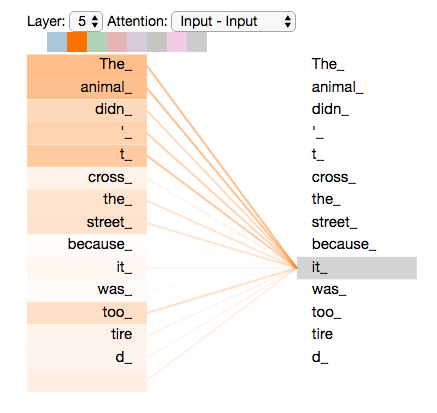
\includegraphics[width=.5\textwidth]{rys03/transformer_attention.png}
		\caption{Mechanizm atencji --- wizualizacja wag poszczególnych słów podczas analizy słowa ,,it''.
			Źródło: https://jalammar.github.io/illustrated-transformer}\label{fig:attention}
	\end{figure}
	
	Równoległe wprowadzanie wszystkich słów wymusza górne ograniczenie na długość zdania.
	Dla większości modeli bazujących na transformerach limit wynosi 512 tokenów.
	Tokenem może być zarówno słowo, jak i część zdania typu przecinek, stąd faktyczny limit liczony w słowach jest jeszcze niższy.
	Jest to mocno ograniczający limit w kontekście wykorzystywanego korpusu, w którym wypowiedzi często złożone są z kilkudziesięciu zdań.
	Problem ten opisywany jest szerzej w rozdziale~\ref{sec:sentences}.

\section{Wektory zdań}
	Modele bazujące na BERT stworzone są z myślą generowania wektorów dla każdego tokena wejściowego.
	Otrzymane w ten sposób wektory kodują informacje semantyczne o wszystkich słowach zdania, jednak nie zawierają informacji o samym zdaniu.
	Jedną z możliwości jest wykorzystanie wartości wektora dla tokena \verb|CLS| --- jest to token wykorzystywany podczas uczenia modelu i reprezentuje znaczenie zdania w kontekście zadań klasyfikacji.
	Można również uśrednić wektory wszystkich słów, jednak nie wszystkie słowa w zdaniu niosą tak samo dużo znaczenia.
	
	Rozwiązanie tego problemu proponują autorzy Sentence-BERT\cite{sbert}.
	Model SBERT złożony jest z dwóch modli BERT połączonych w syjamską sieć.
	Na wyjściu każdego modelu BERT dołożona jest warstwa pooling zwracająca wektor ustalonego rozmiaru dla zdań różnych długości.
	Najlepszą strategią okazała się metoda uśredniania wektorów wszystkich tokenów.
	Następnie wyjściowe dwa wektory wynikowe są łączone i obliczana jest funkcja straty klasyfikatorem \verb|softmax|.
	Architektura ta przedstawiona została na rysunku~\ref{fig:sbert}.
	W celu uzyskania wektorów kodujących semantykę całych zdań, model uczony jest na korpusach zawierających pary zdań oznaczone pod kątem podobieństwa.
	Optymalizuje się odległość między podobnymi zdaniami, jednocześnie maksymalizując odległości między zdaniami różnymi.
	\begin{figure}[ht]
		\centering
		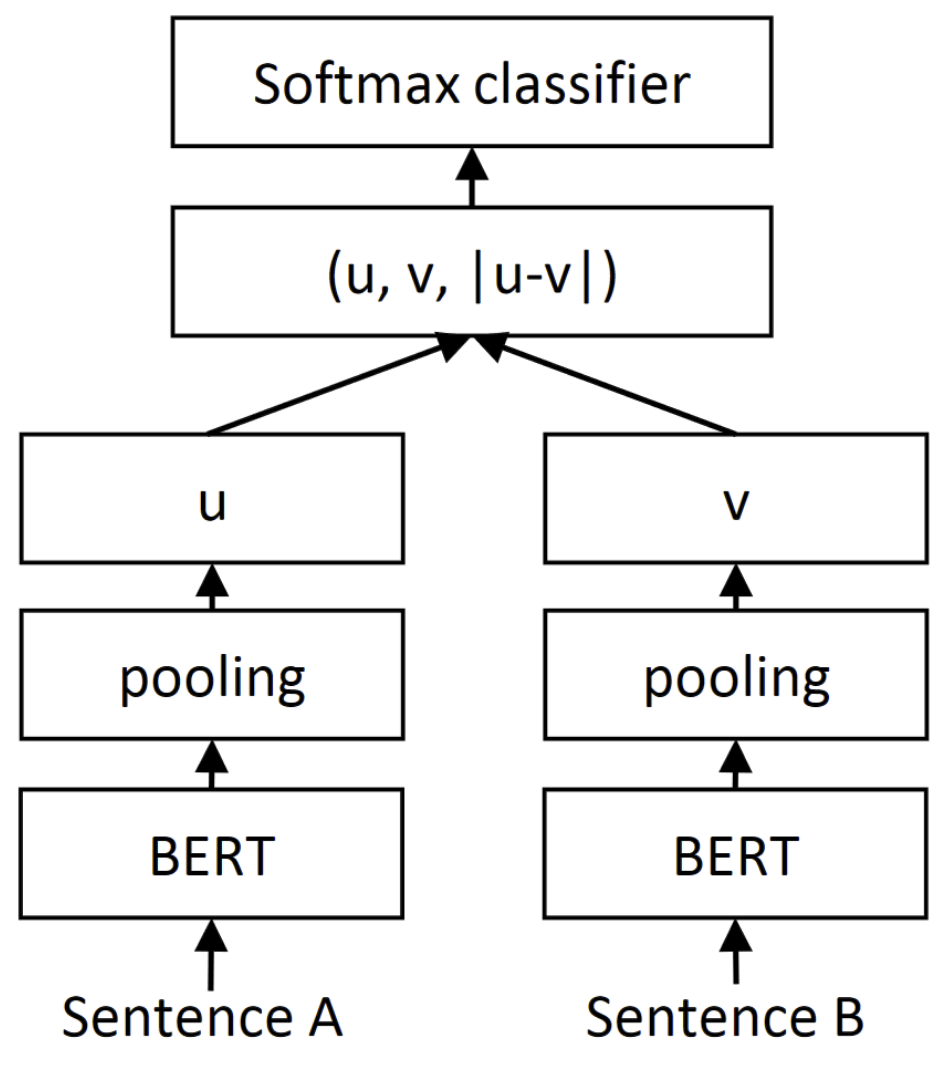
\includegraphics[width=0.3\linewidth]{rys03/sbert.png}
		\caption{Architektura modelu Sentence-BERT\cite{sbert}}\label{fig:sbert}
	\end{figure}

	Ze względu na specyfikę potrzebnego korpusu do trenowania modeli SBERT (oznaczone pary zdań) nie istnieją obecnie modele wytrenowane w języku polskim.
	Jednak w roku 2020 ci sami autorzy opracowali metodę przenoszenia wiedzy (ang.\ \emph{knowledge distillation}) z nauczonego modelu angielskiego na modele wielojęzykowe\cite{sbert_multilingual}.
	Opiera się na koncepcji, według której te same zdania w różnych językach powinny być reprezentowane przez podobne wektory w tej samej przestrzeni.
	Przekazanie wiedzy polega na minimalizacji różnicy wyników między modelem nauczającym, a modelem uczącym się (ang.\ \emph{teacher-student}) --- Rys.~\ref{fig:sbert_multilingual}.
	W tym przykładzie modelem-nauczycielem jest SBERT wytrenowany na angielskim korpusie, natomiast uczniem jest model XLM-R (XLM-RoBERTa).
	Jest to wielojęzykowy model bazujący na architekturze RoBERTa (wariacja BERT stworzona przez Facebook), wytrenowany na 2.5TB danych z CommonCrawl w 100 językach, w tym polskim\cite{xml_r}.
	Model ten zajmuje obecnie ósme miejsce w rankingu KLEJ\footnote{\url{https://klejbenchmark.com/leaderboard} (dostęp dnia 20 maja 2021)}
		oraz drugie miejsce po dostrojeniu (ang.\ \emph{fine-tuning}) na dodatkowych polskich korpusach.
	\begin{figure}[ht]
		\centering
		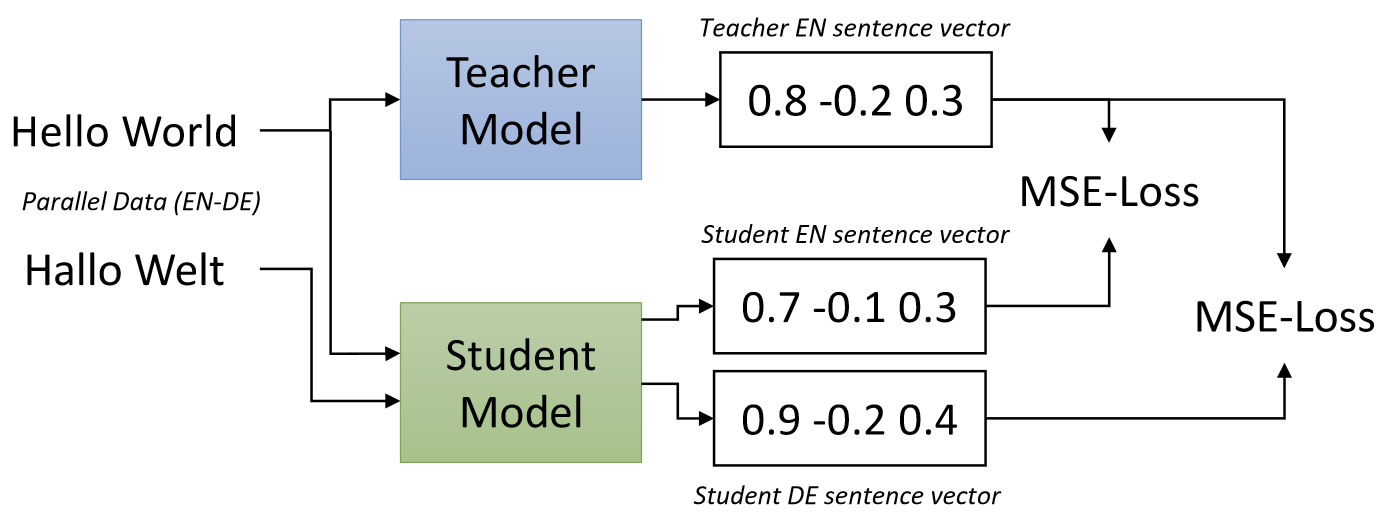
\includegraphics[width=.75\linewidth]{rys03/sbert_multilingual.png}
		\caption{Układ modeli nauczyciel-uczeń w procesie uczenia wielojęzykowego SBERT\cite{sbert_multilingual}}\label{fig:sbert_multilingual}
	\end{figure}
	
	Trenowanie modelu ucznia wymaga par zdań w języku angielskim i języku docelowym.
	Jest to dużo mniejsze ograniczenie, niż w przypadku bezpośredniego uczenia SBERT w docelowym języku.
	Dostępne są wytrenowane modele\footnote{\url{https://www.sbert.net/docs/pretrained_models} (dostęp dnia 20 maja 2021)}, które obejmują również język polski.
	Zostały one uwzględnione w rankingu modeli generujących reprezentacje zdań w języku polskim\cite{sentence_eval}.
	W pracy tej autorzy przetłumaczyli popularny angielski korpus SICK (ang.\ \emph{Sentences Involving Compositional Knowledge})
		zawierający pary zdań oznaczone pod kątem implikacji (ang.\ \emph{entailment}).
	Każda para może być albo powiązana (prawdziwość pierwszego zdania oznacza prawdziwość drugiego), neutralna (pierwsze zdanie nie mówi nic o prawdziwości drugiego), albo sprzeczna.
	Na podstawie tego korpusu stworzono dwa zadania odpowiadające angielskim --- SICK-E (zadanie klasyfikacji) oraz SICK-R (zadanie przewidywania dystrybucji podobieństwa, mierzone miarą korelacji Pearsona).
	
	Na potrzeby tej pracy za najbardziej istotne zadanie uznano SICK-R, ponieważ sprawdza skuteczność oceniania podobieństwa semantycznego dwóch tekstów.
	W tym zadaniu najlepszy wynik uzyskał wielojęzykowy model SBERT \verb|xlm-r-distilroberta-base-paraphrase-v1|
		(aktualne wyniki znajdują się na stronie z kodem źródłowym\footnote{\url{https://github.com/sdadas/polish-sentence-evaluation} (dostęp dnia 20 maja 2021)}).

\section{Wektory wypowiedzi}\label{sec:sentences}
	Modele bazujące na architekturze BERT mają górne ograniczenie na długość zdania wejściowego.
	Wynosi ono 512 tokenów, co odpowiada około 300 słowom.
	Dodatkowo, zbiór danych uczących wykorzystywanych przez modele SBERT zawiera zwykle krótsze zdania,
		przez co skuteczność tych modeli dla pełnego zakresu 512 tokenów może być gorsza niż oczekiwana.
	Jak pokazano na rysunku~\ref{fig:word_count}, wypowiedzi sejmowe są często znacznie dłuższe niż ten limit.
	Mediana liczby słów wynosząca 219 mieści się w limicie, jednak wypowiedzi złożone z więcej niż 300 słów stanowią prawie 39\% zbioru.
  \begin{figure}[ht]
    \begin{minipage}{.75\textwidth}
      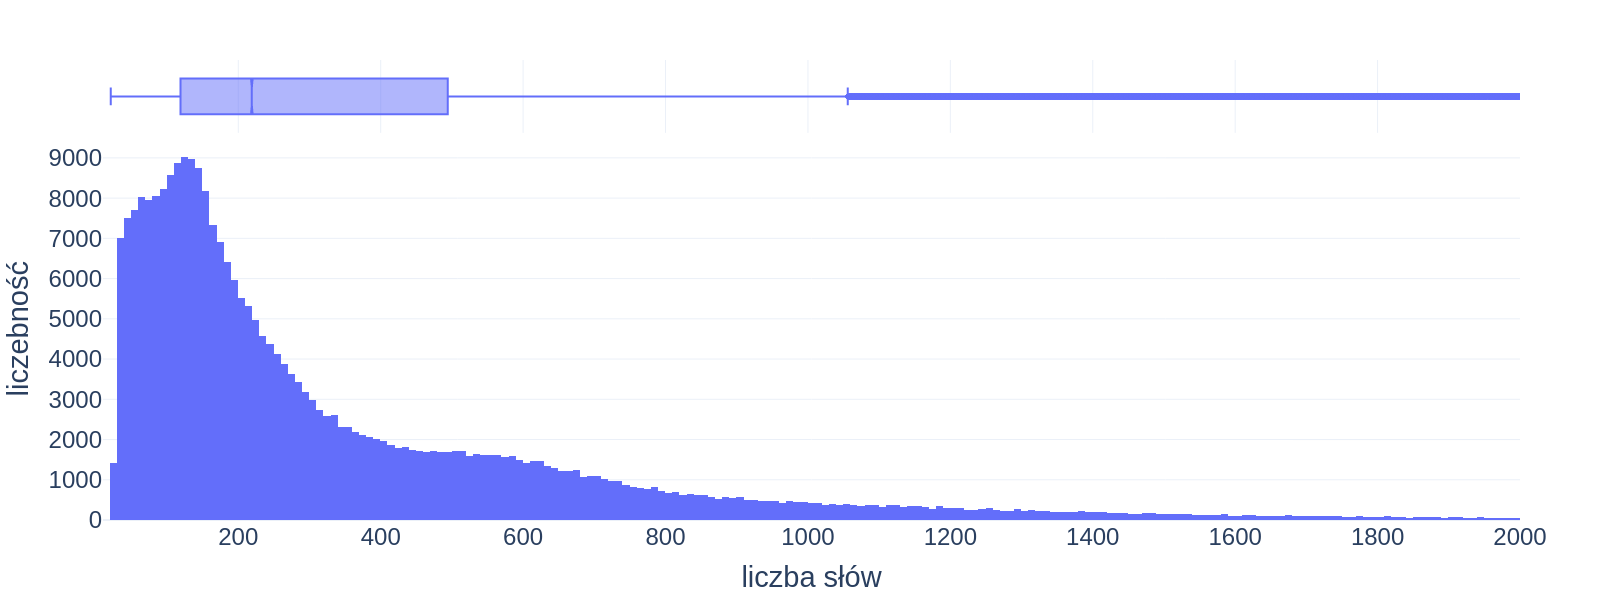
\includegraphics[width=\textwidth]{rys03/word_count.png}
    \end{minipage}%
    \begin{minipage}{.25\textwidth}
      \small
      \begin{tabularx}{\textwidth}{ll}
        Min & 21 \\ 
        Q1 & 119 \\ 
        Mediana & 219 \\
        Q3 & 494 \\ 
        Górny wąs & 1056 \\
        Max & 28.546 \\
      \end{tabularx}
    \end{minipage}
    \caption{Dystrybucja długości wypowiedzi (zakres do 2000 słów)}\label{fig:word_count}
  \end{figure}

	Z tego powodu postanowiono dzielić wypowiedzi na zdania, generować wektory dla każdego zdania, a następnie połączyć je w jeden wektor wynikowy dla całej wypowiedzi.
	Rozważono następujące strategie:
	\begin{itemize}
		\item średnia,
		\item średnia ważona,
		\item wektor pierwszy w rankingu,
		\item średnia pierwszych pięciu wektorów w rankingu
	\end{itemize}
	Do wygenerowania wag oraz rankingu potrzebna jest metoda oceniająca, na ile istotne jest każde zdanie w kontekście całej wypowiedzi.
	Stworzono w tym celu dwie metody: jedna wykorzystująca algorytm LexRank oraz druga wykorzystująca TF-IDF\@.

	\subsection{LexRank}
		LexRank\cite{LexRank} to stworzony w 2004r.\ stochastyczny algorytm bazujący na teorii grafów, służący do generowania podsumowań długich tekstów.
		Jako podsumowanie traktowany jest zbiór najistotniejszych zdań z tekstu --- jest to metoda ekstrakcyjna, która nie zmienia struktury zdań.
		Istnieją nowe metody bazujące na uczeniu maszynowym, które jako podsumowanie generują nowy tekst zawierający sens dokumentu,
			jednak na potrzeby tej pracy wymagany jest algorytm przypisujący wagi oryginalnym zdaniom.
		
		Algorytm konstruuje graf, gdzie wierzchołki odpowiadają zdaniom, a ich wartość obliczana jest algorytmem TF-IDF\@.
		Krawędzie grafu odpowiadają wartości podobieństwa między dokumentami i mierzone są na miarą kosinusową.
		Wizualizacja takiego grafu przedstawiona została na rysunku~\ref{fig:lexrank}.
		\begin{figure}[ht]
			\centering
			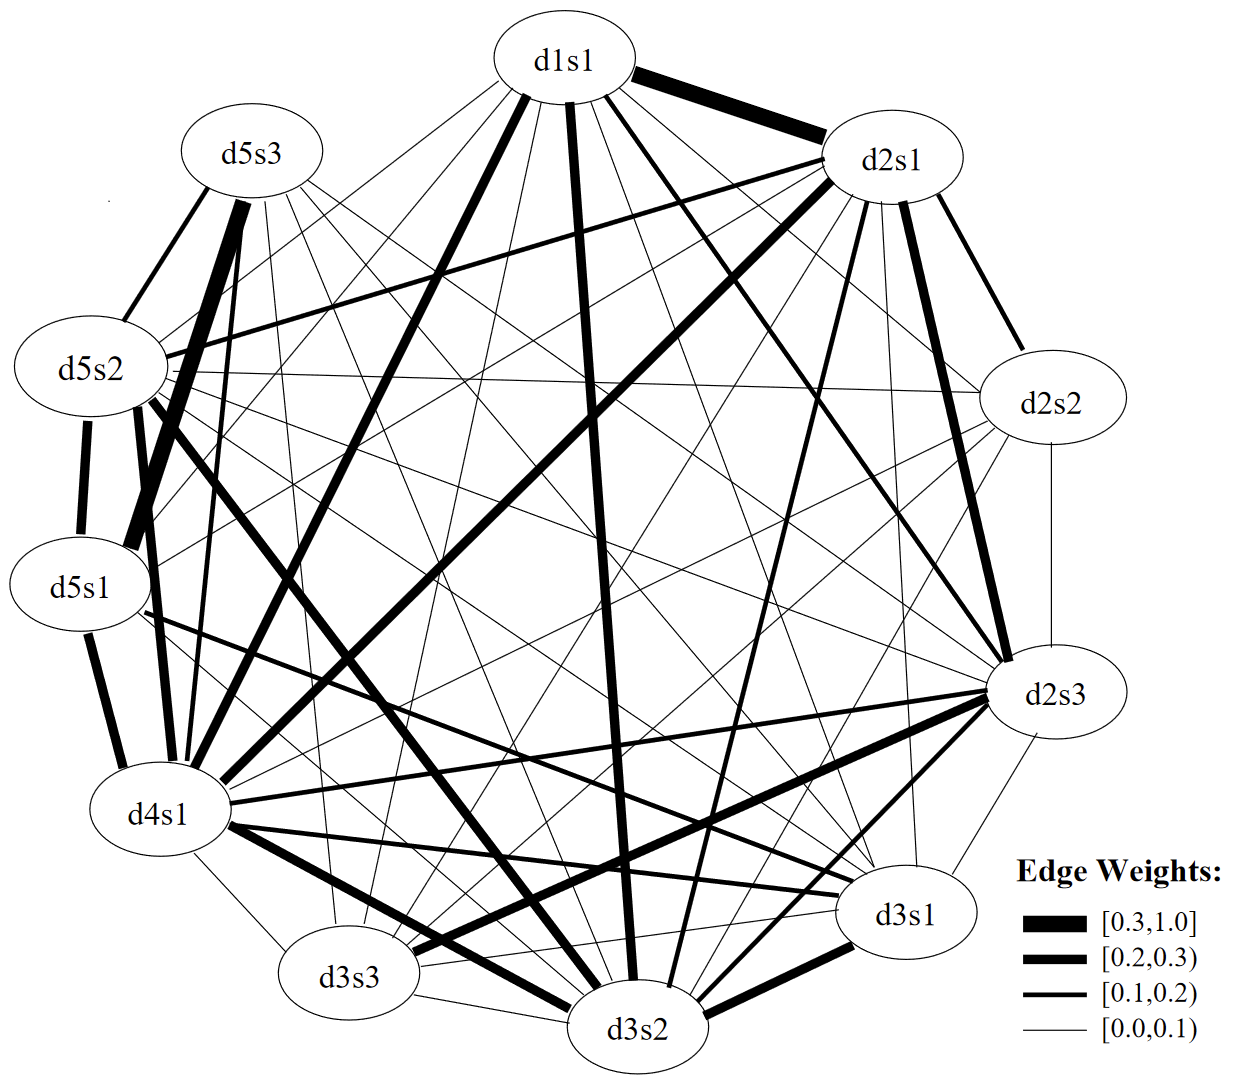
\includegraphics[width=0.5\linewidth]{rys03/lexrank.png}
			\caption{Graf ważony miarą podobieństwa między zdaniami (wierzchołkami)\cite{LexRank}}\label{fig:lexrank}
		\end{figure}
		Graf przedstawiony w postaci macierzy, po znormalizowaniu wierszy, jest macierzą stochastyczną
			(macierz kwadratowa, w której każdy wiersz sumuje się do wartości 1), którą można potraktować jako łańcuch Markova.
		Udowodnione jest, że łańcuch Markova jest zbieżny do rozkładu stacjonarnego, jeśli spełniony jest następujący warunek:
		\[\lim_{x \to \infty}X^n = 1^T r\]
		gdzie \(X\) to macierz stochastyczna, a \(r\) to rozkład stacjonarny łańcucha Markova.
		Rozkład stacjonarny można interpretować jako prawdopodobieństwo że skończymy na danym elemencie przechodząc przez łańcuch, niezależnie od stanu początkowego.
		Możemy go więc potraktować jako wektor centralny (ang.\ \emph{centrality vector}),
			gdzie wartość każdego elementu informuje, jak bardzo centralne jest zdanie na danej pozycji.

		W oryginalnej pracy autorzy mierzyli odległości pomiędzy wektorami TF-IDF\@.
		Nic nie stoi jednak na przeszkodzie, aby w ich miejsce wstawić wektory wygenerowane przez model BERT\@.
		Otrzymany w ten sposób wektor centralny posłuży jako wagi wektorów zdań oraz jako ranking.

	\subsection{TF-IDF}
		Alternatywną metodę ważenia zdań oparto na metodzie TF-IDF\@.
		TF odnosi się do \emph{term-frequency} i oznacza częstość występowania danego słowa w dokumencie.
		IDF oznacza \emph{inverse document-frequency}, zawiera wartości dla każdego słowa, informujące jak bardzo jest ono powszechne.
		Im w większej liczbie dokumentów występuje dane słowo, tym mniej informacji niesie o konkretnym dokumencie.
		Wartość IDF obliczana jest według następującego wzoru:
		\[idf(t)=\log\left(\frac{1+n}{1+df(t)}\right) + 1\]
		gdzie \(t\) oznacza słowo, \(n\) to liczba wszystkich dokumentów, a \(df(t)\) to częstość występowania słowa we wszystkich dokumentach.
		Wartość \(tfidf(t)\) obliczana jest jako iloczyn \(tf(t)\) i \(idf(t)\).
		
		W pierwszym kroku wyuczono model na całym korpusie, aby skonstruować pełen słownik oraz wartości macierzy IDF\@.
		Następnie podczas generowania wektorów wypowiedzi, obliczana jest macierz tf-idf, gdzie wierszami są kolejne zdania.
		Dla każdego zdania kolumny są sumowane, dzięki czemu otrzymujemy wektor o długości równej liczbie zdań oznaczający,
			na ile znaczące są słowa w zdaniu w kontekście całego korpusu (macierz IDF zawiera wartości uwzględniające wszystkie dane).
		Sama ta wartość nie może posłużyć jednak do porównywania zdań, gdyż dłuższe zdania będą miały wyższy wynik, nawet jeśli będą złożone z samych nieznaczących słów.
		Podzielenie tych wartości przez liczę wykrytych słów w danym zdaniu (liczbę niezerowych kolumn w danym wierszu macierzy tf-idf) będzie miało odwrotny efekt
			--- preferowane będą krótkie zdania z małą liczbą słów o wysokim wyniku tf-idf.
		Dłuższe zdania, które mogą zawierać istotne informacje, będą miały niski wynik, gdyż naturalnie składają się również z mniej znaczących słów.
		Postanowiono więc zbadać, jak zmienia się suma wartości tf-idf w zależności od liczby wykrytych słów.
		Zależność ta przedstawiona została na wykresie~\ref{fig:tfidf_sent}a.
		Poprzez aproksymację punktową do danych dopasowana została funkcja potęgowa narysowana na wykresie kolorem czerwonym.
		Aproksymacji poddane zostały trzy współczynniki według następującego wzoru funkcji:
		\[a\cdot x^b + c\]
		dzięki czemu otrzymano następującą funkcję, której dobrym przybliżeniem jest pierwiastek kwadratowy:
		\[1.003\cdot x^{0.486} - 0.065\]
		Odzwierciedla ona średnią sumę wartości tf-idf dla danej długości zdania.
		Można więc przyjąć, że zdania poniżej tej krzywej są mniej istotne, niż zdania powyżej.
		Wartości wszystkich zdań normalizowane są wartością tej funkcji, dzięki czemu nie są promowane ani długie zdania, ani krótkie.
		Znormalizowane wartości zdań przedstawione zostały na wykresie~\ref{fig:tfidf_sent}b.
		Wartości te użyte zostały jako wagi wektorów BERT oraz jako ranking zdań.

		\begin{figure}[htb]
			\centering
			\begin{minipage}{.5\textwidth}
				a)\par\medskip % chktex 10
				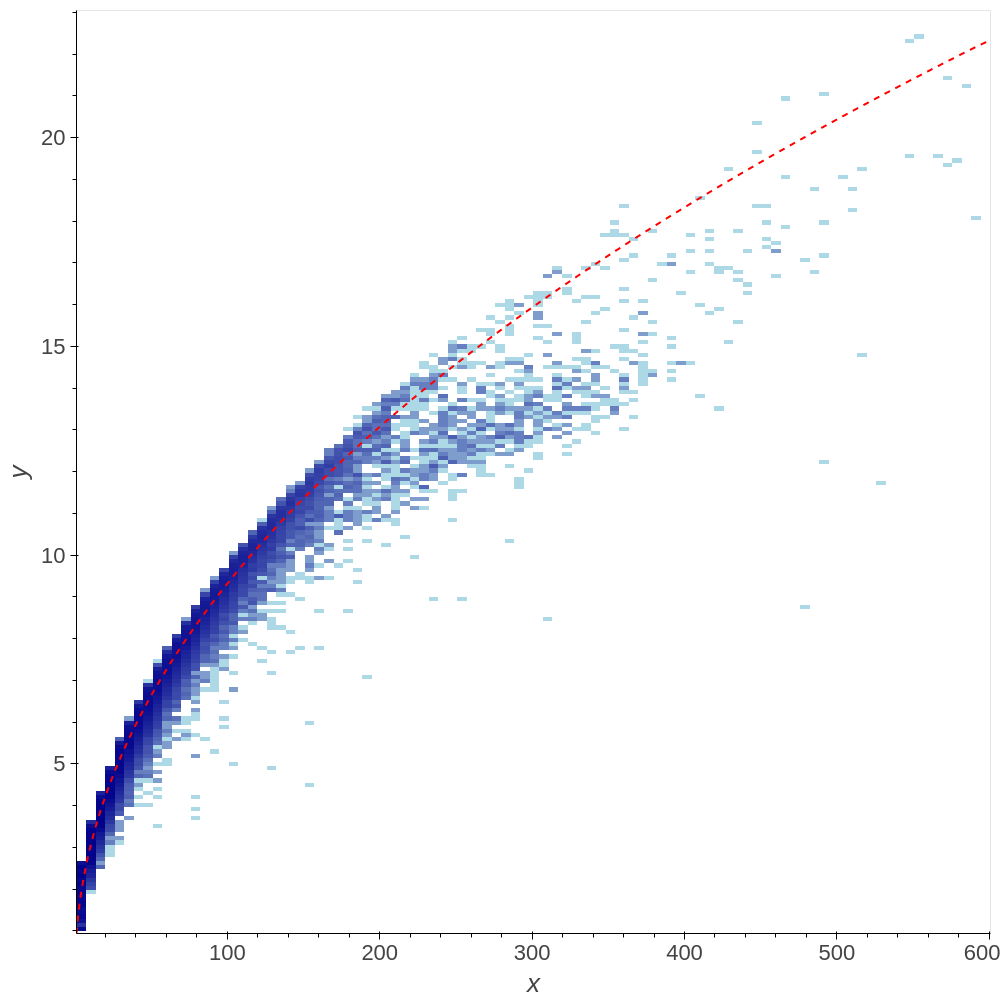
\includegraphics[width=\linewidth]{rys03/tfidf.png}
			\end{minipage}%
			\begin{minipage}{.5\textwidth}
				b)\par\medskip % chktex 10
				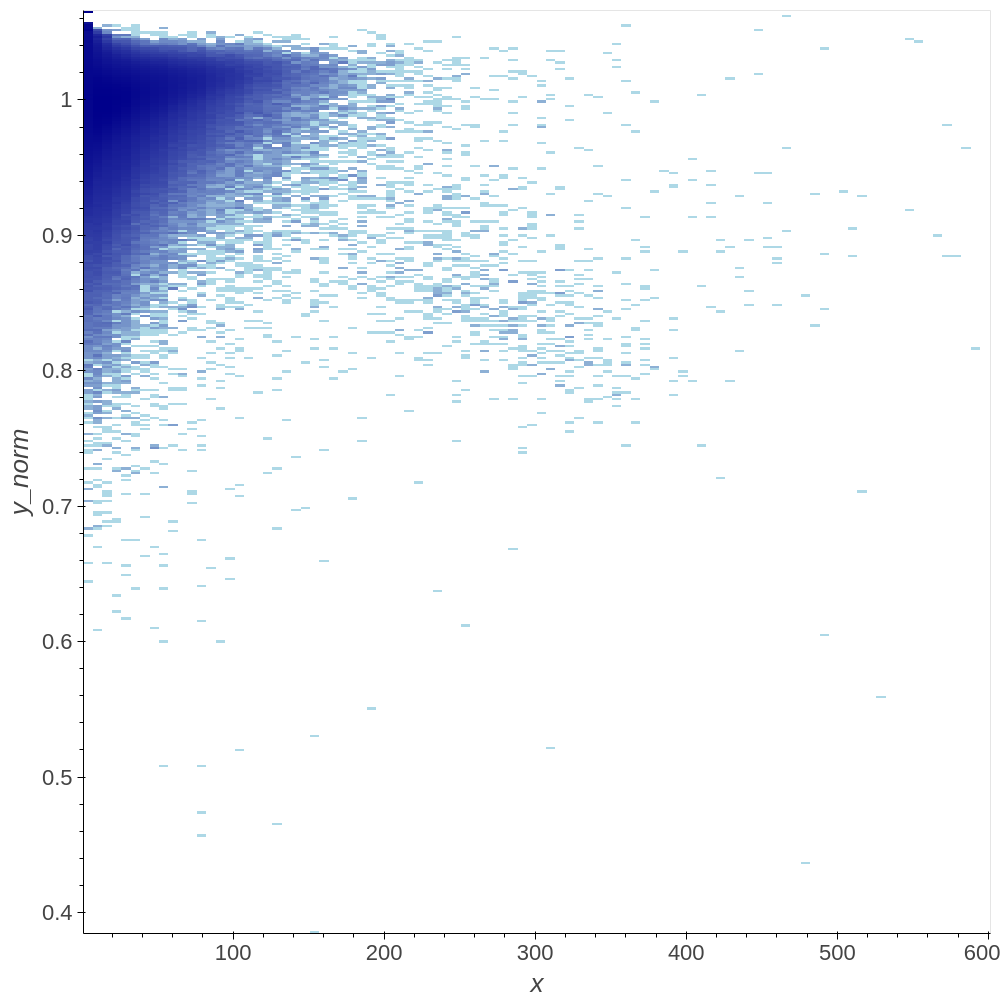
\includegraphics[width=\linewidth]{rys03/tfidf_norm.png}
			\end{minipage}
			\caption{Suma wartości tf-idf w zależności od liczby wykrytych słów (zakres do 600 słów):
				a) dane nieznormalizowane z dopasowaną krzywą, b) dane znormalizowane krzywą}\label{fig:tfidf_sent} % chktex 9 chktex 10
		\end{figure}

\section{Alternatywne rozwiązania}
	Modele oparte o transformery zajmują obecnie wysokie miejsca w rankingach, jednak nie są to jedyne metody dające dobre wyniki.
	W celu porównania wyników wygenerowano wektory dwoma alternatywnymi metodami --- siecią konwolucyjną oraz standardowym TF-IDF\@.

	\subsection{Sieć konwolucyjna}
		Sieci konwolucyjne wykorzystują warstwy połączone filtrami konwolucyjnymi nakładanymi na lokalne cechy.
		Początkowo wykorzystywane do zagadnień związanych z przetwarzaniem obrazów,
			znalazły zastosowanie również w pozostałych dziedzinach uczenia maszynowego, w tym NLP\@.
		W 2019r. Google udostępniło wielojęzykowy wariant modelu USE (ang.\ \emph{Universal Sentence Encoder})\cite{use_multilingual} wspierający 16 języków, w tym polski.
		W pracy tej opisano dwa warianty --- jeden wykorzystujący CNN oraz drugi opierający się na transformerach.
		Model oparty na transformerach osiągnął drugi najlepszy wynik w zadaniu SICK-R w polskim rankingu Polish Sentence Evaluation\cite{sentence_eval}.
		Wersja CNN modelu jest szybsza kosztem mniejszej dokładności.
		Umożliwia ona jednak kodowanie znacznie dłuższych zdań (256 tokenów kontra 100).
		Oba modele wytrenowane zostały na danych zebranych z forów dyskusyjnych (w postaci pytania i odpowiedzi)
			oraz na zbiorze SNLI (Stanford Natural Language Inference) przetłumaczonym na pozostałe 15 języków za pomocą Google Translate.

	\subsection{TF-IDF}
		W przeciwieństwie do omawianych wyżej modeli, w przypadku TF-IDF długość wypowiedzi działa na korzyść algorytmu.
		Im dłuższa wypowiedź, tym większa szansa na uzyskanie kombinacji słów dokładniej identyfikującej dokument.
		Algorytm ten nie posiada żadnego górnego ograniczenia na długość dokumentu.
		Algorytm podczas zliczania liczby wystąpień danego słowa nie bierze pod uwagę odmian słów,
			przez co słowa ,,budżet'' i ,,budżetu'' są traktowane jako osobne kategorie.
		Jest to szczególnie istotne w językach słowiańskich, ponieważ wykorzystywanych jest w nich mnóstwo odmian słów.
		
		Aby zminimalizować wynikającą z tego działania utratę informacji, zdecydowano się wstępnie przetworzyć dokumenty przed zliczeniem słów.
		Wykorzystano w tym celu polski model do biblioteki \verb|spaCy|
			--- \verb|pl_spacy_model_morfeusz|\cite{spacy_pl} udostępniony przez Instytut Podstaw Informatyki Polskiej Akademii Nauk\footnote{\url{http://zil.ipipan.waw.pl/SpacyPL} (dostęp dnia 21 maja 2021)}.
		Biblioteka umożliwia między innymi lematyzację (sprowadzenie słowa do formy podstawowej) każdego słowa w zdaniu.
		Wykorzystuje przy tym wyuczony model, który rozpoznaje strukturę zdania --- przykładowo, czy dane słowo jest w danym kontekście rzeczownikiem, czy czasownikiem.
		Następnie na podstawie tej wiedzy może określić formę podstawową słowa.
		Polski model na tym etapie wykorzystuje słownik morfologiczny Morfeusz2\cite{morfeusz}.
		Zbudowany jest on na danych ze Słownika gramatycznego języka polskiego.

		Podczas tokenizacji dokumentów generowane są również n-gramy z zakresu (1,3).
		Oznacza to, że zliczane będą również wystąpienia dwóch oraz trzech kolejnych słów (np. ,,Unia Europejska'', ,,Rzecznik praw obywatelskich'').
		Dodatkowo, przyjęto próg odrzucenia \verb|min_df| równy 5 oznaczający, że dany token musi wystąpić w minimum pięciu dokumentach,
			aby był uwzględniony w wynikowej macierzy.

% !TeX root = ./Dyplom.tex
% chktex-file 21

\chapter{Modelowanie tematyczne}\label{sec:topic_modeling}
	Modele tematyczne (ang.\ \emph{topic modeling}) służą do organizowania, wyjaśniania, analizy w czasie, przeszukiwania i streszczania dużych zbiorów danych.
	Odbywa się to poprzez wynajdywanie podobieństw między dokumentami w korpusie.
	Najpopularniejszą metodą modelowania tematów jest LDA (ang.\ \emph{Latent Dirichlet Allocation})\cite{LDA}.
	Jest to generatywny model probabilistyczny.
	Dokonuje dyskretyzacji ciągłej przestrzeni tematów na z góry określoną liczbę \emph{t} tematów
		i modeluje dokumenty jako kombinację tematów, dla każdego określając prawdopodobieństwo, że dokument jest na dany temat.
	Równocześnie każdy temat jest rozkładem prawdopodobieństwa wystąpienia słów.
	Wiąże się to z pewnymi problemami, mianowicie często największe prawdopodobieństwo wystąpienia mają powszechne słowa nie niosące istotnej informacji, np.\ zaimki czy łączniki.
	Problem ten jest częściowo rozwiązywany listą nieinformatywnych słów (ang.\ \emph{stop words}), które są odfiltrowywane z dokumentów.
	Często lista ta musi być dopasowana do danego zbioru tekstów.
	Dokumenty reprezentowane są jako zbiór słów, w którym zliczane jest wystąpienie każdego słowa --- BOW (ang.\ \emph{bag-of-words}).
	Wadą takiego formatu jest fakt, że nie zachowuje informacji o kolejności słów, ani ich semantyce.

	Celem LDA jest znalezienie takich tematów, które mogą posłużyć do odtworzenia oryginalnych rozkładów słów z dokumentów z minimalnym błędem.
	Model nie rozróżnia pomiędzy słowami informatywnymi, a nieinformatywnymi, ma za zadanie jedynie jak najlepiej odzwierciedlać oryginalne dokumenty.
	Z tego powodu najbardziej prawdopodobne słowa w temacie niekoniecznie odzwierciedlają faktyczne tematy dokumentów.
	Na podstawie analizy LDA otrzymujemy nie tylko klasyfikację dokumentu do tematu, lecz cały wektor prawdopodobieństw przynależności dokumentu do każdego z tematów.
	Wektor ten ma więc rozmiar równy liczbie wszystkich tematów.
	Jak pokazano w~\cite{BoW_PL}, nadzorowane metody klasyfikacji wykorzystujące te wektory dają podobne wyniki do metod opartych o \emph{word-to-vec}.

	Modele oparte o transformery osiągają najlepsze wyniki w wielu zagadnieniach z dziedziny NLP\cite{KLEJ},
		więc powstały również bazujące na nich metody modelowania tematycznego.
	Jedną z nich jest BERTopic\cite{BERTopic}, algorytm generujący tematy na podstawie wektorów BERT\@.
	Wykorzystuje UMAP\cite{UMAP} w celu redukcji wymiarowości wektorów do 5 wymiarów.
	Następnie za pomocą algorytmu HDBSCAN\cite{HDBSCAN} wektory grupowane są w klastry.
	Każda grupa reprezentuje pewien temat.
	Reprezentacje tematów generowane są za pomocą wariantu TF-IDF\@,
		gdzie wszystkie dokumenty w klastrze traktowane są jako jeden dokument i porównywane między sobą.
	Poszczególne etapy rozwinięte zostały w kolejnych podrozdziałach.

\section{Redukcja wymiarów}
	Wektory powstałe w wyniku analizy wypowiedzi za pomocą SBERT mają 768 wymiarów.
	W przypadku wykorzystania USE jest to 512 wymiarów, natomiast wektory TF-IDF mają tyle wymiarów,
		ile jest wszystkich tokenów w korpusie (dla wykorzystywanego korpusu jest to ponad 2mln).
	Wykorzystywany algorytm grupowania HDBSCAN działa lepiej na danych w mniejszym wymiarze,
		autorzy testowali algorytm do 50 wymiarów\cite{HDBSCAN}.
	Z tego powodu konieczna jest redukcja wymiaru danych.
	
	Wykorzystano w tym celu algorytm UMAP (ang.\ \emph{Uniform Manifold Approximation and Projection})\cite{UMAP}.
	Oparty jest on o techniki topologicznej analizy danych bazując na geometrii riemannowskiej.
	Konstruuje rozmytą reprezentację topologiczną wysokowymiarowych danych,
		a następnie optymalizuje reprezentację tych danych w docelowym wymiarze tak,
		aby jej rozmyta reprezentacja topologiczna była jak najbardziej podobna mierząc entropią krzyżową.
	W ten sposób algorytm dąży do tego, aby dane w niskowymiarowej przestrzeni jak najlepiej odzwierciedlały topologiczną strukturę oryginalnych danych.
	Dzięki temu zachowane są zarówno lokalne, jak i globalne zależności między danymi.

	Redukcja do zbyt niskiego wymiaru może skutkować zbyt wielkiej utracie informacji,
		podczas gdy redukcja do większego wymiaru może dawać gorsze rezultaty podczas grupowania.
	Postanowiono redukować dane do pięciu wymiarów, tak jak sugeruje autor BERTopic\cite{BERTopic}.
	Podczas redukcji wymiarowości wektorów SBERT i USE korzystano z metryki kosinusowej.
	Dla wektorów TF-IDF zastosowano metrykę Hellingera, która mierzy podobieństwo rozkładów prawdopodobieństwa
		(wektory tf-idf można traktować jak prawdopodobieństwo znalezienia danego tokenu w dokumencie).
	
	Istotnym parametrem algorytmu UMAP jest \verb|n_neighbors|.
	Balansuje on między skupieniem się na lokalnej strukturze danych, a globalną strukturą.
	Ogranicza liczbę sąsiadujących wektorów, które są analizowane podczas nauki struktury rozmaitości topologicznej danych.
	Dla niskich wartości koncentruje się na lokalnej strukturze nie biorąc pod uwagę pełnego obrazu danych.
	Wysokie wartości skutkują utratą szczegółów, ukazując bardziej ogólne zależności.
	Wpływ tego parametru zobrazowany został na rysunku~\ref{fig:umap} dla wartości 5, 15 oraz 100.
	Dla niskiej wartości parametru \verb|n_neighbors| powstało wiele lokalnych grup o niskiej liczebności.
	Wraz ze wzrostem wartości parametru lokalne grupy łączą się w coraz większe klastry.

	\begin{figure}[htb]
		\centering
		\begin{minipage}{.33\textwidth}
			a)\par\medskip % chktex 10
			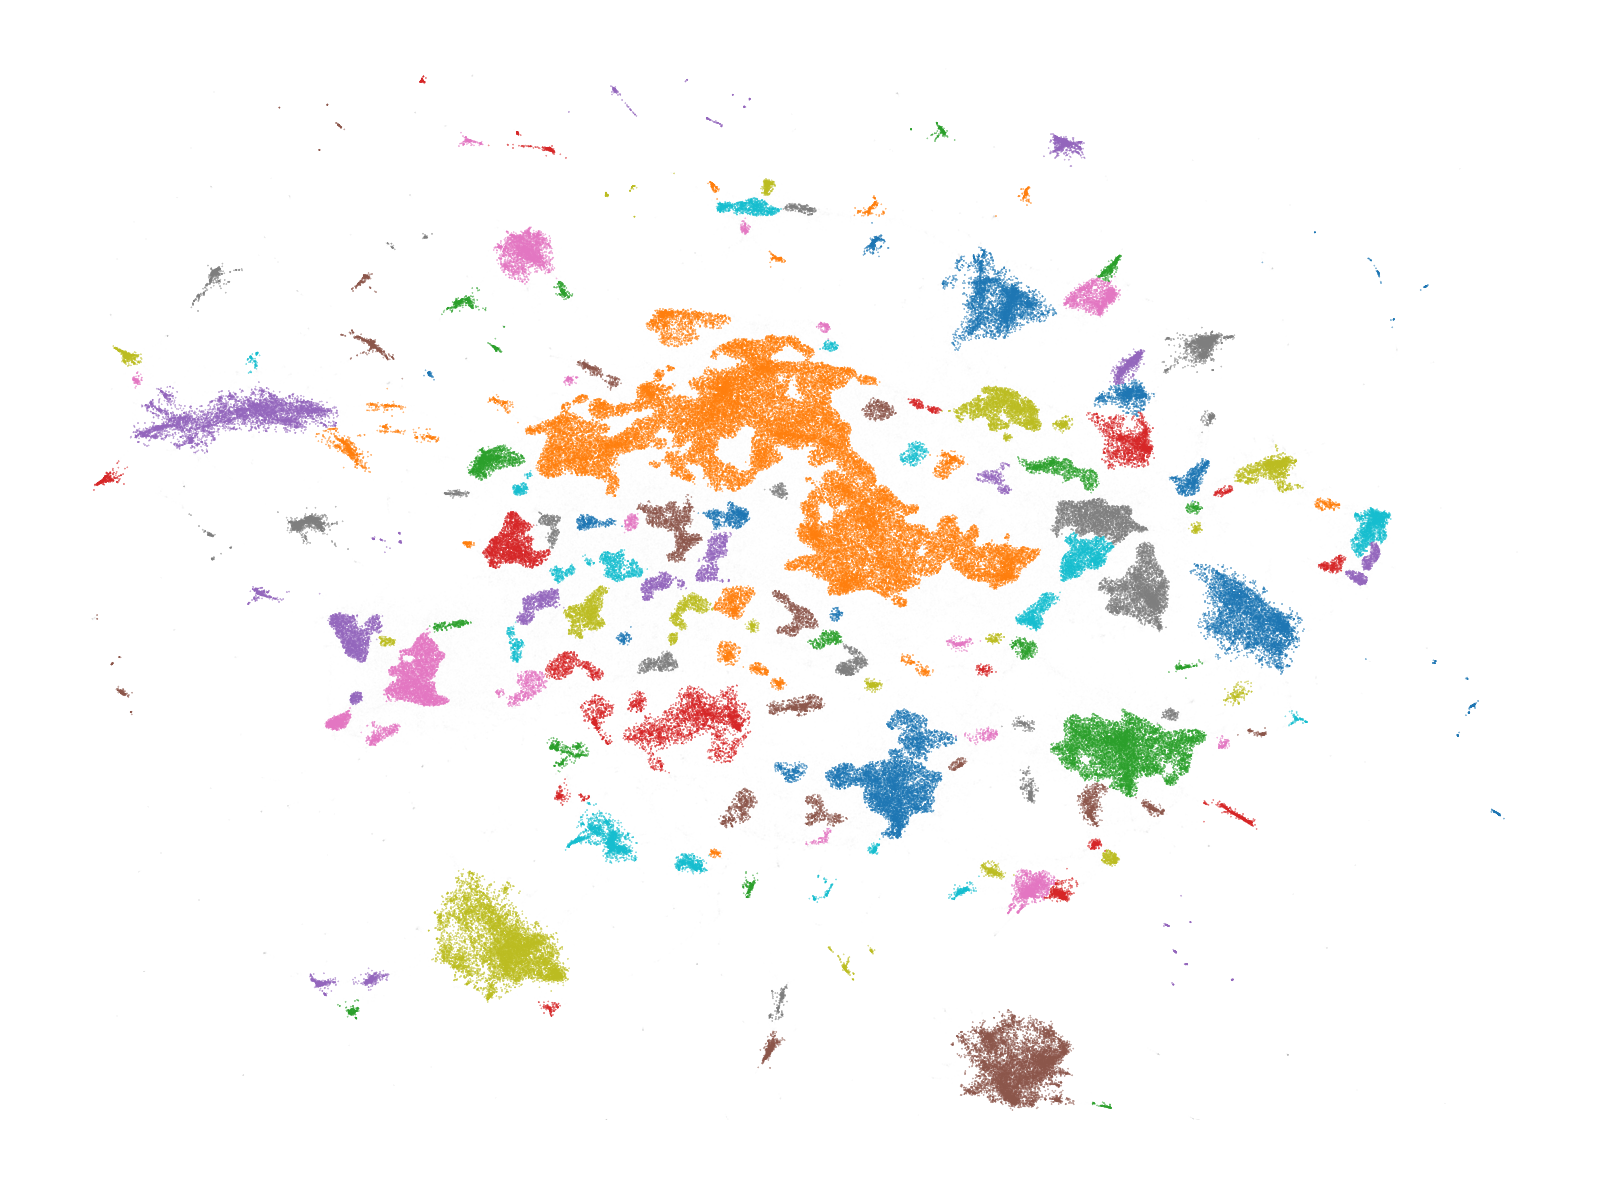
\includegraphics[width=\linewidth]{rys04/umap_5_100_100.png}
			n\_neighbors = 5
		\end{minipage}%
		\begin{minipage}{.33\textwidth}
			b)\par\medskip % chktex 10
			
\includegraphics[width=\linewidth]{rys04/umap_15_100_100.png}
			n\_neighbors = 15
		\end{minipage}%
		\begin{minipage}{.33\textwidth}
			c)\par\medskip % chktex 10
			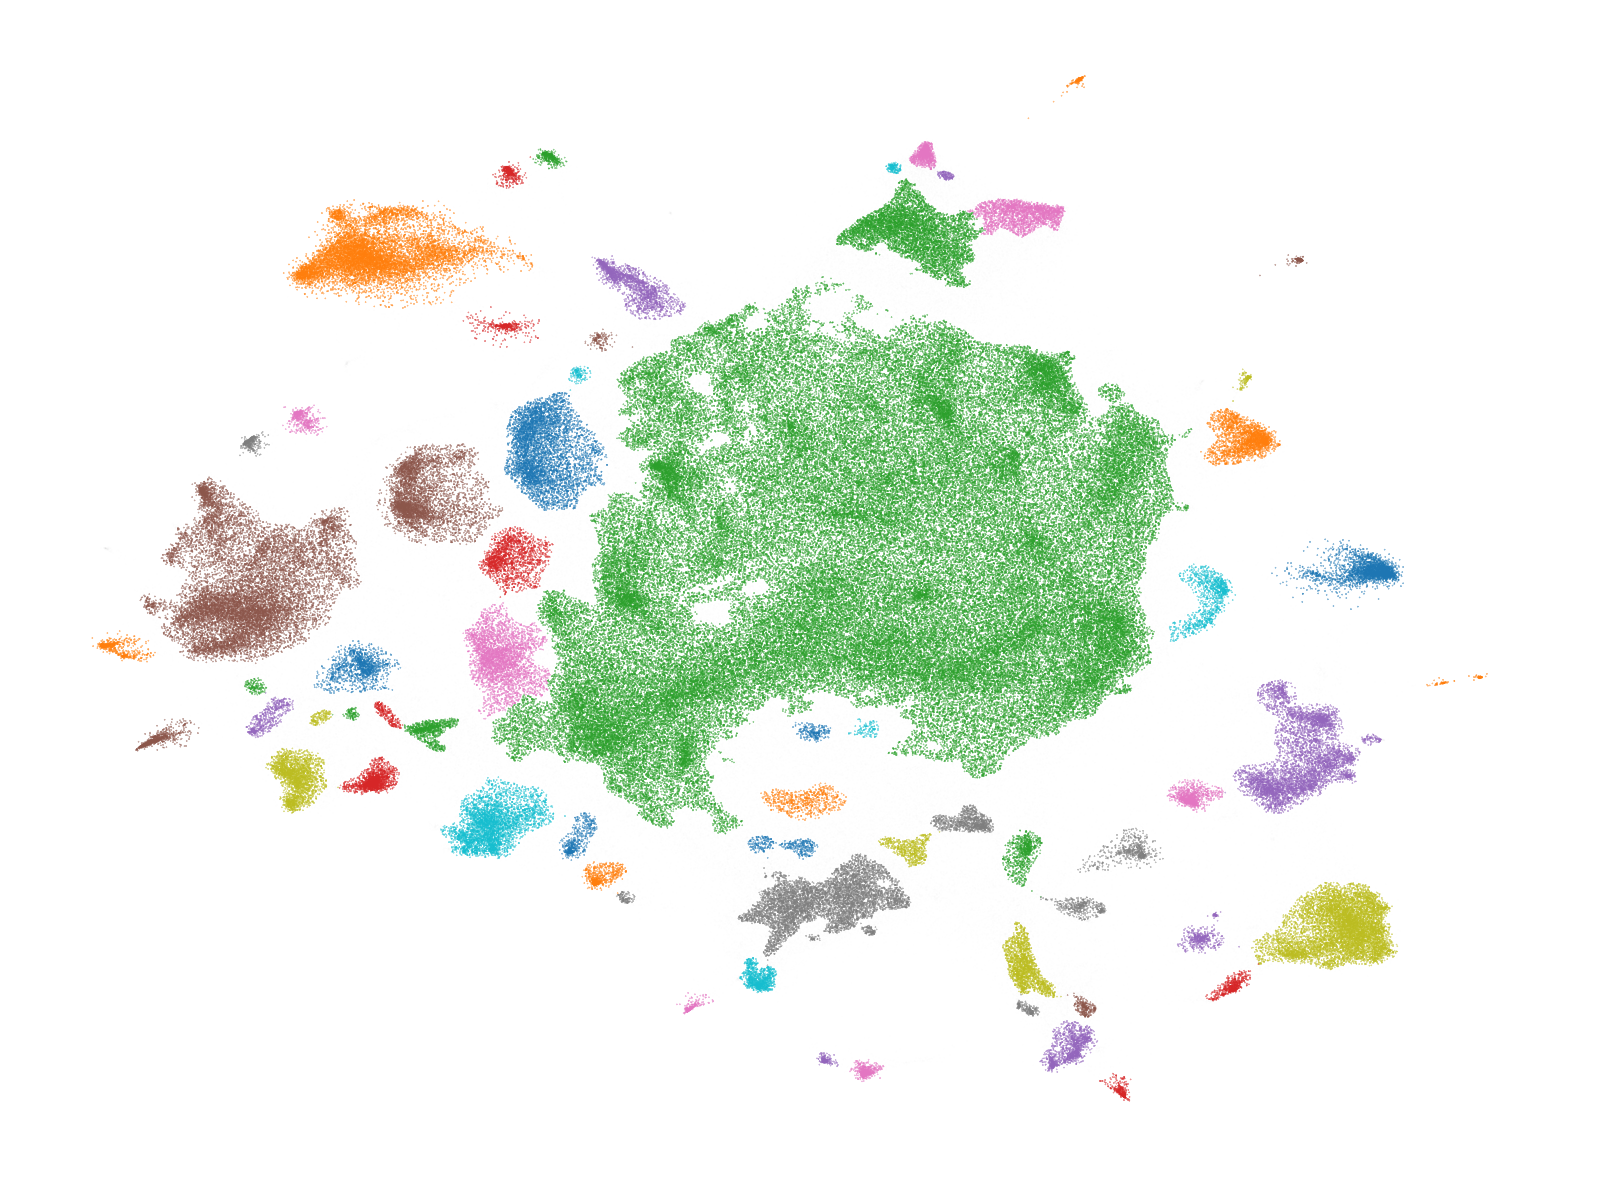
\includegraphics[width=\linewidth]{rys04/umap_100_100_100.png}
			n\_neighbors = 100
		\end{minipage}
		\caption[Dwuwymiarowa reprezentacja danych przez UMAP]{Dwuwymiarowa reprezentacja danych przez UMAP w zależności od wartości parametru n\_neighbors.
			Kolory odpowiadają klastrom wykrytym przez HDBSCAN (dla minimalnego rozmiaru klastra równego 100).}\label{fig:umap}
	\end{figure}
	

\section{Grupowanie}\label{sec:hdbscan}
	HDBSCAN to algorytm klastrowania hierarchicznego bazujący na DBSCAN (ang.\ \emph{Density-based spatial clustering of applications with noise}).
	W celu zobrazowania działania algorytmu, wybrano ograniczony podzbiór danych.
	Z klastrów wykrytych na wszystkich danych wylosowano pięć, a z każdego z nich wylosowano dziesięć wektorów.
	Dodatkowo, wybrano dziesięć losowych wektorów bez przypisanego klastra.
	W ten sposób otrzymano 60 dokumentów, które poddano ponownej analizie HDBSCAN
		(wykorzystując wektory uzyskane z redukcji wymiarów wszystkich dokumentów do pięciu).
	
	Algorytm określa klastry jako rejony o większej gęstości otoczone rzadziej rozmieszczonymi punktami.
	Aby określić gęstość używana jest metryka odległości do najbliższego \emph{k}-tego sąsiada oznaczona dalej jako \(core_k(x)\).
	Na jej podstawie stworzono metrykę określającą odległość wzajemnej osiągalności (ang.\ \emph{mutual reachability distance}):
	\[ d_k(a,b) = \max \left\lbrace core_k(a),core_k(b),d(a,b) \right\rbrace \]
	gdzie:
	\begin{itemize}
		\item \(core_k(x)\) odległość do najbliższego \emph{k}-tego sąsiada,
		\item \(d(a,b)\) pierwotna metryka odległości.
	\end{itemize}
	Dzięki takiej metryce punkty które są blisko siebie pozostają w pierwotnych odległościach, natomiast rzadsze punkty są od siebie odpychane.

	Na podstawie obliczonych odległości konstruowane jest minimalne drzewo rozpinające algorytmem Prima.
	Wierzchołkami grafu są punkty danych, a wagami krawędzi obliczone odległości.
	Na rys.~\ref{fig:mst} przedstawiono powstałe drzewo dla wyselekcjonowanych danych.
	Zgodnie z oczekiwaniami, punkty nieprzypisane pierwotnie do żadnego klastra mają znacznie większe odległości od punktów, które tworzą zbiory.
	Widać też, że klastry nie nachodzą na siebie, a więc dane są dobrze odseparowane.
	
	\begin{figure}[htb]
		\centering
		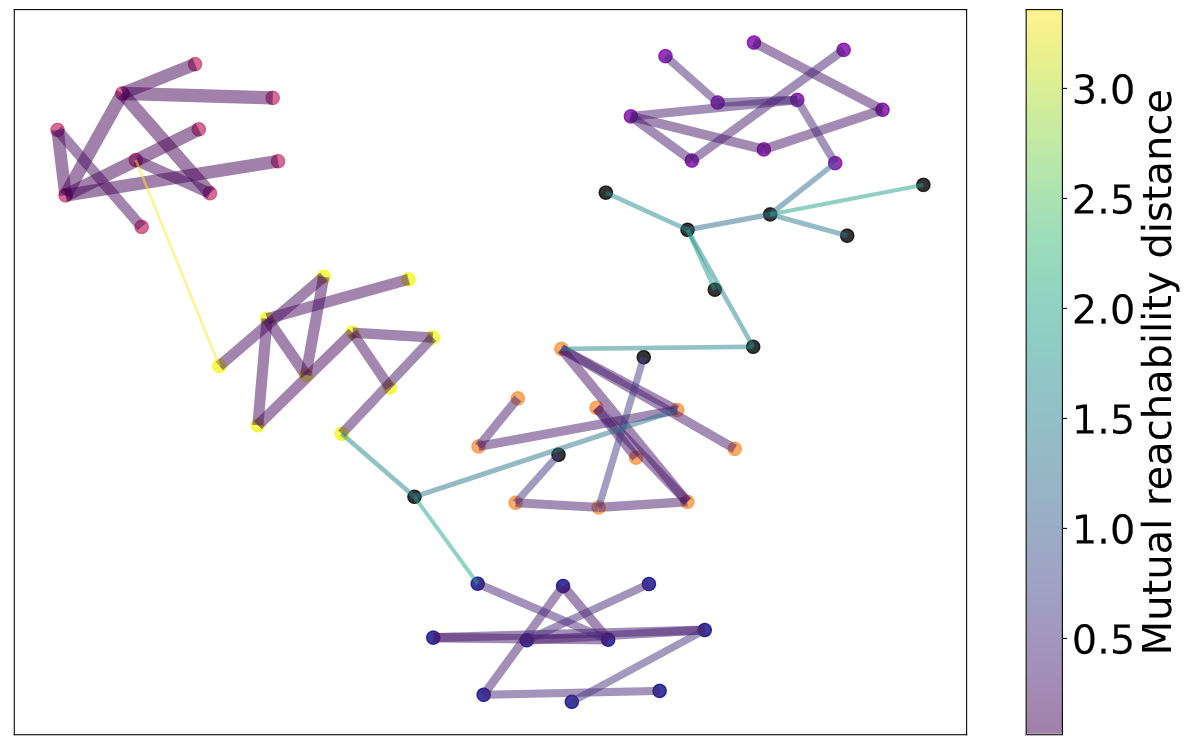
\includegraphics[width=0.5\linewidth]{rys04/hdbscan_mst.png}
		\caption[Minimalne drzewo rozpinające]{Minimalne drzewo rozpinające. Grubość krawędzi i kolor zależy od wartości odległości, gdzie grubsze linie oznaczają mniejszą odległość.
			Punkty pokolorowane są zgodnie z pierwotnymi klastrami, a na czarno zaznaczone są punkty, które nie miały klastrów.}\label{fig:mst}
	\end{figure}
	
	Następnie powstałe krawędzie łączone są w hierarchiczne grupy, poprzez scalanie kolejnych krawędzi o najmniejszej odległości.
	Powstałą w ten sposób hierarchię klastrów można zobrazować jako dendrogram (rys.~\ref{fig:dendrogram}a).
	Celem algorytmu jest jednak otrzymanie zbioru klastrów, nie hierarchii.
	W tym celu HDBSCAN kondensuje hierarchię do mniejszego drzewa.
	Algorytm analizuje hierarchię i podczas każdego podziału sprawdza powstałe dwie grupy.
	Jeśli obie grupy mają rozmiar większy niż minimalny (minimalny rozmiar klastra to parametr algorytmu \verb|min_cluster_size|),
		to taki wynik takiego podziału jest traktowany jako dwie prawdziwe grupy.
	Jeśli jednak któraś z powstałych grup ma mniejszy rozmiar niż minimalny to uznaje się,
		że są to punkty wypadające z klastra niestanowiące osobnej grupy i pozostawiana jest jedynie większa grupa.
	W ten sposób otrzymuje się dużo mniej grup, które wraz ze wzrostem odległości między punktami zmniejszają swój rozmiar.
	Wynik takiego działania przedstawiony jest na rysunku~\ref{fig:dendrogram}b.
	
	\begin{figure}[htb]
		\centering
		\begin{minipage}{.5\textwidth}
			a)\par\medskip % chktex 10
			\begin{flushleft}
				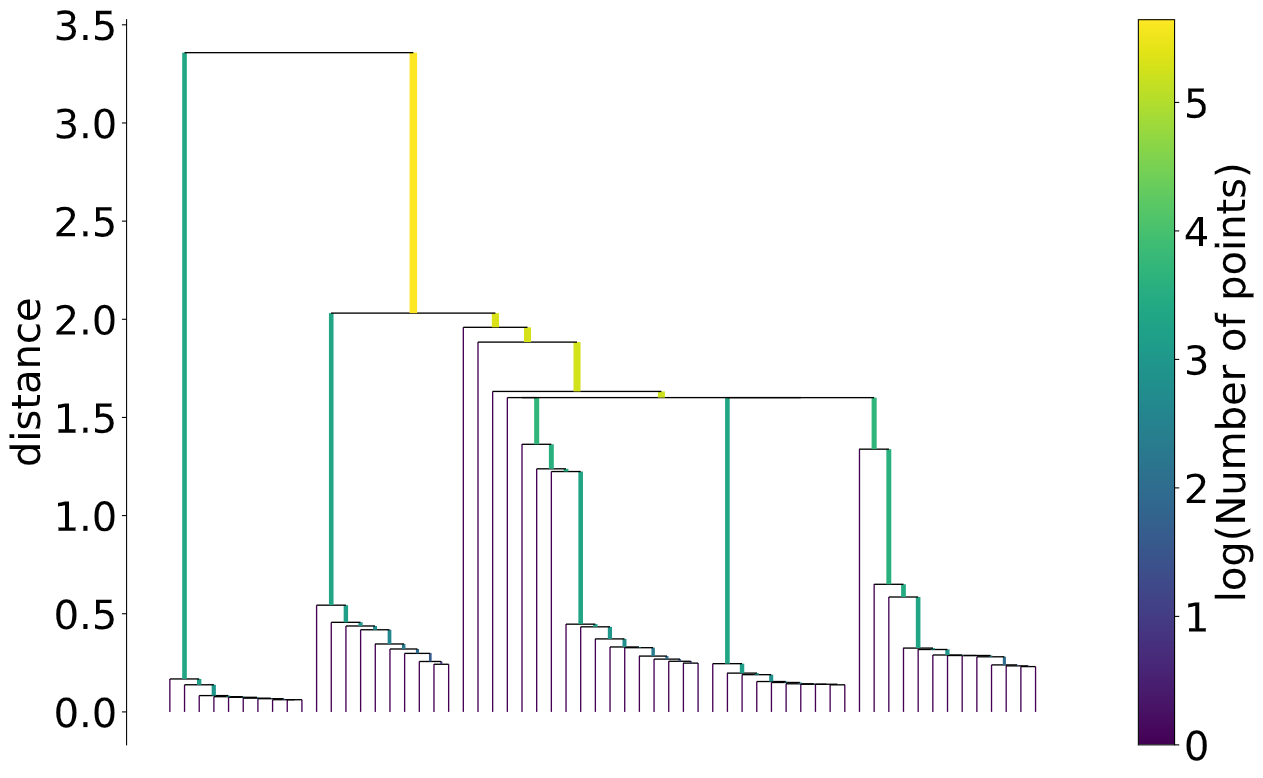
\includegraphics[width=.95\linewidth]{rys04/hdbscan_slt.png}
			\end{flushleft}
		\end{minipage}%
		\begin{minipage}{.5\textwidth}
			b)\par\medskip % chktex 10
			\begin{flushright}
				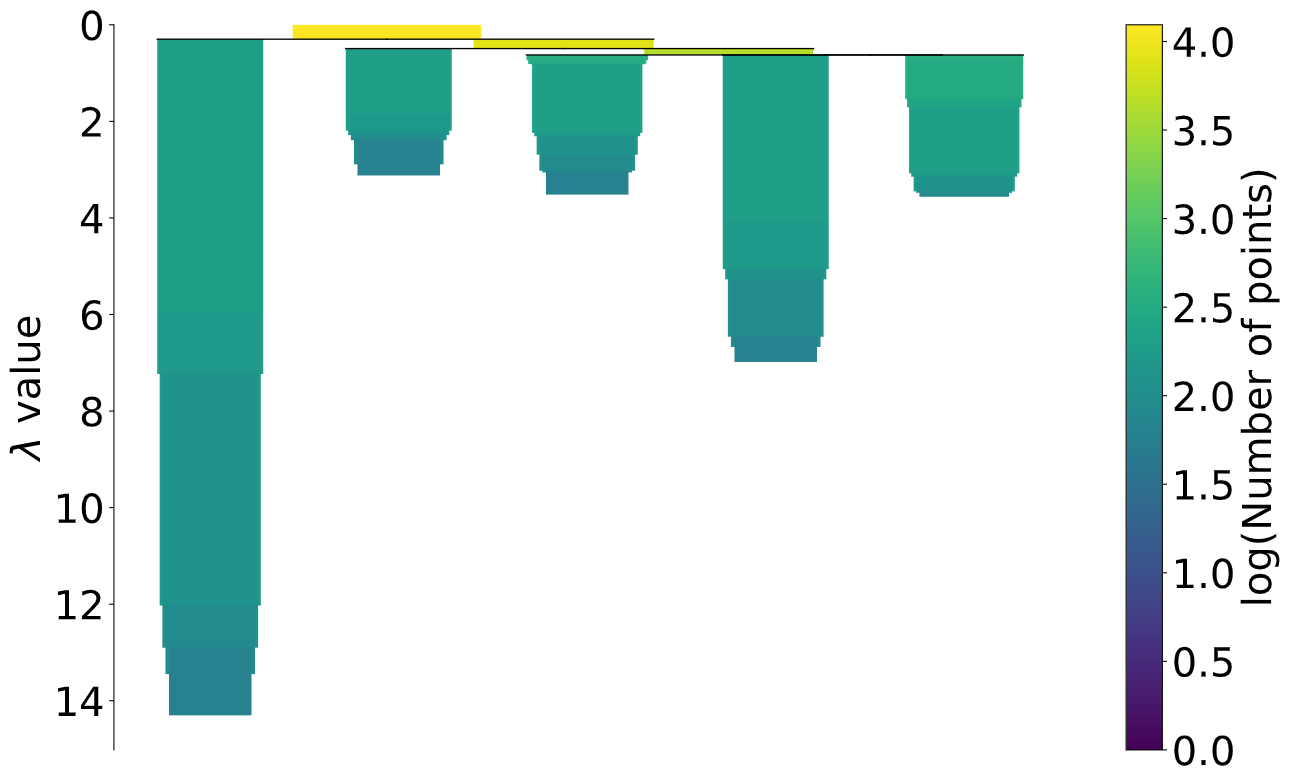
\includegraphics[width=.95\linewidth]{rys04/hdbscan_ct.png}
			\end{flushright}
		\end{minipage}
		\caption[Dendrogramy hierarchii klastrów]{Dendrogramy hierarchii klastrów: a) na podstawie drzewa rozpinającego, b) skondensowane}\label{fig:dendrogram} % chktex 9 chktex 10
	\end{figure}

	Na końcu z powstałego skondensowanego drzewa wybierane są najstabilniejsze klastry.
	Stabilność klastra określona na podstawie wartości \(\lambda=\frac{1}{distance}\).
	Dla każdego klastra możemy oznaczyć \(\lambda_{birth}\) i \(\lambda_{death}\) jako wartości \(\lambda\)
		odpowiednio w momencie powstania klastra i rozbicia na mniejsze klastry.
	Dla każdego punktu \(p\) w klastrze, możemy zdefiniować \(\lambda_p\)
		jako wartość \(\lambda\) w momencie, w którym punkt odłączył się od klastra, gdzie \(\lambda_{birth} < \lambda_p < \lambda_{death}\).
	Następnie dla klastra obliczamy jego stabilność jako:
	\[ \sum_{p\in cluster}\left(\lambda_p - \lambda_{birth}\right) \]

	Aby wybrać końcowe klastry najpierw zaznaczane są wszystkie liście drzewa.
	Jeśli suma stabilności dwóch łączących się klastrów jest większa niż stabilność powstałego klastra, 
		to ustawiamy stabilność klastra na tą sumę.
	Natomiast jeśli stabilność złączonego klastra jest większa niż jego potomków, to wybieramy ten klaster i odznaczamy wszystkich potomków.
	W ten sposób zaznaczamy kolejne klastry aż dojdziemy do korzenia drzewa, a powstałe zaznaczenie to zbiór klastrów.
	Na rysunku~\ref{fig:dendrogram}b zaznaczonych zostałoby pięć klastrów w kolorze morskim.
	Pozostałe punkty nienależące do tych klastrów uznawane są za szum i nie mają przypisanych grup.

	Parametr \emph{k} w implementacji algorytmu HDBSCAN nazwany jest \verb|min_samples| 
		i domyślnie jego wartość jest równa wartości \verb|min_cluster_size|.
	Na rysunku~\ref{fig:umap} wartość ta była równa 100.
	Zmniejszenie wartości \verb|min_samples| do 1 skutkuje wykryciem większej ilości mniejszych grup.
	Rezultat redukcji z takim parametrem przedstawiony został na rys.~\ref{fig:hdbscan}a.

	Rys~\ref{fig:hdbscan}b przedstawia klastry wykryte na pięciowymiarowych wektorach, a następnie zwizualizowane na dwóch.
	Wykrywanie klastrów w przestrzeni pięciowymiarowej pozwala na dokładniejsze wykrycie zależności między punktami danych,
		które mogą zostać utracone przy redukcji do zbyt małej liczby wymiarów.
	W szczególności, punkty oznaczone jako szum w pięciu wymiarach, w dwóch wymiarach wykrywane są jako klastry.
	
	\begin{figure}[htb]
		\centering
		\begin{minipage}{.5\textwidth}
			a)\par\medskip % chktex 10
			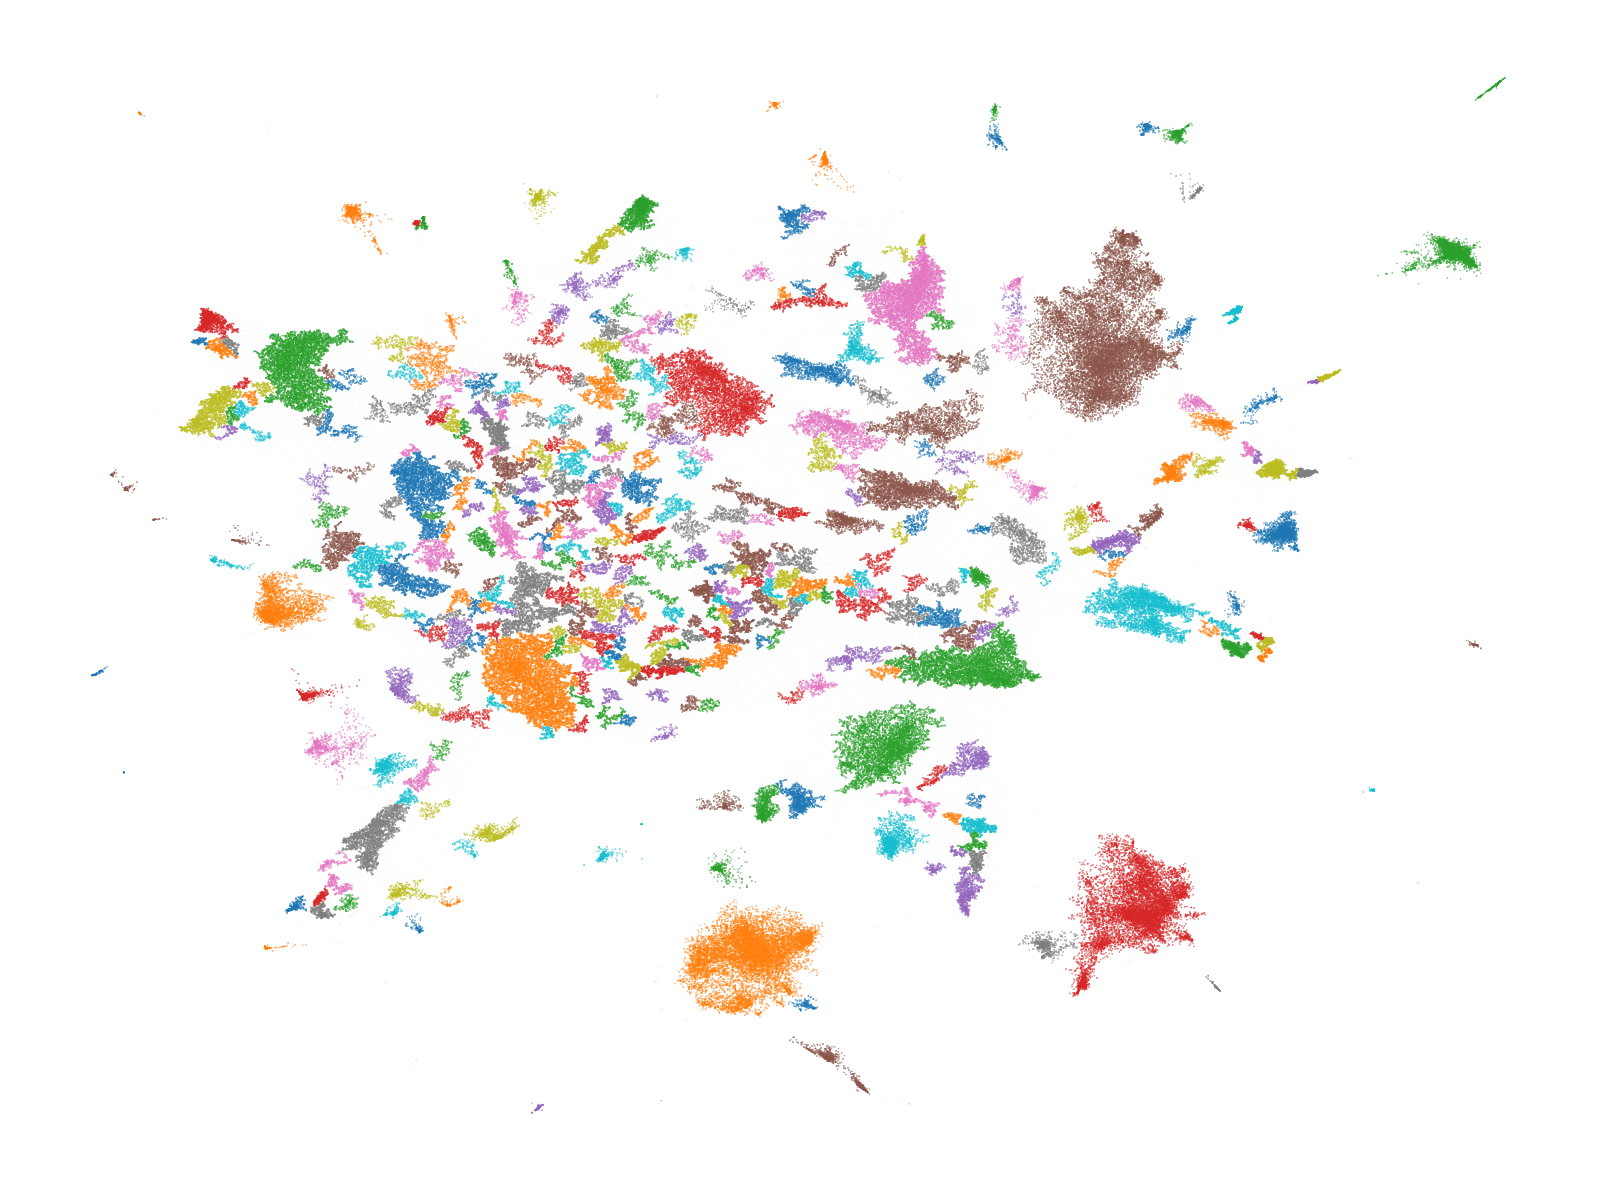
\includegraphics[width=\linewidth]{rys04/umap_15_100_1.png}
		\end{minipage}%
		\begin{minipage}{.5\textwidth}
			b)\par\medskip % chktex 10
			
\includegraphics[width=\linewidth]{rys04/umap_15_100_1_5d.png}
		\end{minipage}
		\caption[Klastry wykryte przez HDBSCAN]{Klastry wykryte przez HDBSCAN dla \emph{min\_samples} równego 1 na wektorach: a) dwuwymiarowych, b) pięciowymiarowych}\label{fig:hdbscan} % chktex 9 chktex 10
	\end{figure}

\section{Reprezentacja tematu}
	Każdy temat reprezentowany jest zbiorem słów najlepiej opisujących zawarte w nim dokumenty.
	Jednocześnie słowa te powinny być specyficzne dla danego zbioru tak, aby widoczne były różnice między tematami.
	Jest to problem podobny do wyszukiwania słów identyfikujących dokument algorytmem TF-IDF\@.
	Tym razem jednak chcemy znaleźć słowa identyfikujące zbiór dokumentów na tle innych zbiorów.
	Autor BERTopic nazwał tą wariację algorytmu c-TF-IDF\cite{BERTopic} (ang.\ \emph{class-based TF-IDF}):
	\[c-TF-IDF_i = \frac{t_i}{w_i} \cdot \log \frac{m}{\sum_j^n t_j} \]
	gdzie:
	\begin{itemize}
		\item \(t_i\) częstość występowania słowa \emph{t} w klasie \emph{i},
		\item \(w_i\) liczba słów w klasie \emph{i},
		\item \(m\) liczba wszystkich pierwotnych dokumentów (niezgrupowanych),
		\item \(\sum_j^n t_j\) suma częstości występowania słowa \emph{t} we wszystkich klasach.
	\end{itemize}

	W ten sposób uzyskano ranking wszystkich słów w danej klasie.
	Na podstawie tego rankingu wybiera się od pięciu do dziesięciu słów z najwyższym wynikiem, które stanowią reprezentację tematu.
	Często zdarza się jednak, że otrzymane słowa będą bardzo podobne.
	Przykładowe reprezentacje powstałe tą metodą przedstawione zostały w tabeli~\ref{tab:mmr}a.
	Aby zminimalizować liczbę podobnych słów w reprezentacji tematu i jednocześnie zdywersyfikować jego opis,
		w BERTopic zastosowany jest algorytm MMR (ang.\ \emph{Maximal Marginal Relevance})\cite{MMR}:
	\[MMR = \arg \max_{D_i \in R\backslash S} \left[\lambda\left(Sim_1(D_1, Q) - (1-\lambda) \max_{D_j \in S} Sim_2(D_i, D_j)\right)\right]\]
	gdzie:
	\begin{itemize}
		\item \(D_i\) analizowany kandydat,
		\item \(R\backslash S\) zbiór kandydatów, bez już wybranych,
		\item \(\lambda\) stała w zakresie \(\left[0,1\right]\), kontrolująca zróżnicowanie wyników (0 dla maksymalnie zdywersyfikowanych, 1 dla listy odpowiadającej wzięciu wprost najlepszych wyników),
		\item \(S\) zbiór już wybranych kandydatów,
		\item \(Q\) zapytanie,
		\item \(Sim_1\) metryka podobieństwa kandydata do zapytania,
		\item \(Sim_2\) metryka podobieństwa kandydatów między sobą.
	\end{itemize}
	W kontekście poszukiwania najlepszej reprezentacji tematu, kandydatami są słowa z najwyższymi wynikami \emph{c-TF-IDF}, a zapytanie to wektor całego tematu.
	Wektor tematu obliczany jest wybranym modelem SBERT kodującym dokument powstały z połączenia trzydziestu słów tematu o najwyższych wynikach \emph{c-TF-IDF}.
	Natomiast jako obie metryki \(Sim_1\) i \(Sim_2\) wykorzystywane jest podobieństwo kosinusowe.
	Wartość parametru \(\lambda\) ustawiono na 0 (maksymalna dywersyfikacja).
	W ten sposób otrzymuje się reprezentacje tematów dużo lepiej opisujące zbiory,
		co jest szczególnie istotne w języku polskim zawierającym wiele odmian tych samych słów.
	Tabela~\ref{tab:mmr}b przedstawia reprezentacje tematów otrzymane po zastosowaniu MMR\@.

	\begin{table}[htb]
		\caption{Reprezentacje wybranych tematów: a) bez MMR, b) z MMR}\label{tab:mmr} % chktex 9 chktex 10
		\centering
		a) % chktex 10
		\begin{tabularx}{.9\textwidth}{rl}
			\toprule
			A	&	morskich | statków | morskiego | statku | morskiej	\\ 
			B	&	lotnicze | lotnictwa | lotniczego | lotnisk | lotniczych	\\ 
			C	&	celnego | celnych | towarów | celne | celny	\\
			\midrule
		\end{tabularx}

		b) % chktex 10
		\begin{tabularx}{.9\textwidth}{rl}
			A	&	statków | statkach | marynarzy | gospodarki morskiej | administracji morskiej	\\ 
			B	&	lotnicze | lotnictwa | lotnictwa cywilnego | prawo lotnicze | ruchu lotniczego \\ 
			C	&	celnego | celnych | prawo celne | kodeks celny | prawa celnego \\
			\bottomrule
		\end{tabularx}
	\end{table}
% !TeX root = ./Dyplom.tex
% chktex-file 9
% chktex-file 21

\chapter{Ocena skuteczności modeli}
	Analizowane algorytmy są nienadzorowane, co oznacza, że nie ma jednoznacznej metody oceny wyników.
	Jedyną metodą ewaluacji modeli tematycznych dającą pewność jest manualna weryfikacja poprzez np.\ ocenianie w trzystopniowej skali,
		które reprezentacje tematów są spójne, a które nie.
	Jest to jednak kosztowna metoda, dlatego tworzy się algorytmy dające dobre przybliżenie ocen człowieka.
	Ocena spójności tematów według takich algorytmów porównywana jest z ocenami człowieka poprzez współczynnik korelacji Pearsona.

	Alternatywną metodą zaproponowaną w~\cite{Word_intrusion} jest podmiana słowa w reprezentacji tematu (ang.\ \emph{word intrusion task}).
	W wygenerowanych zestawach słów podmieniane jest jedno słowo na losowe.
	Następnie uczestnicy badania muszą zidentyfikować podmienione słowo.
	Jeśli tematy są spójne, to niepasujące słowo powinno być łatwe do zidentyfikowania,
		natomiast w mniej spójnych tematach słowa będą sprawiały wrażenie bardziej losowych, co utrudni poprawne rozwiązanie problemu.

\section{Ewaluacja spójności reprezentacji tematów}\label{sec:coherence_scores}
	Najpopularniejszą metodą ewaluacji wygenerowanych tematów jest analiza reprezentacji tematów (zbioru słów opisujących temat).
	Im lepiej słowa opisujące temat reprezentują wszystkie dokumenty w danym temacie, tym lepszy model.
	W pracy~\cite{U_MASS} autorzy proponują algorytm (zwany dalej \(C_{UMass}\))
		analizujący pary słów z reprezentacji tematu pod kątem współwystępowania w dokumentach korpusu.
	Jeśli para słów często występuje razem w dokumentach, to są one powiązane.
	Można więc określić spójność całej reprezentacji tematu badając wszystkie w niej zawarte pary słów.
	Miara ta porównana została z wynikami zadania podmiany słowa i uzyskała ona lepszą korelację z ocenami ludzi.
	Wykres dla \emph{n\_neighbors} równego 15 przedstawiony został na rys.~\ref{fig:umass_score}.
	Format parametrów na osi x na tym wykresie i wszystkich kolejnych jest następujący: <n\_neighbors>: <min\_cluster\_size>, <min\_samples>.

	\begin{figure}[htb]
		\centering
		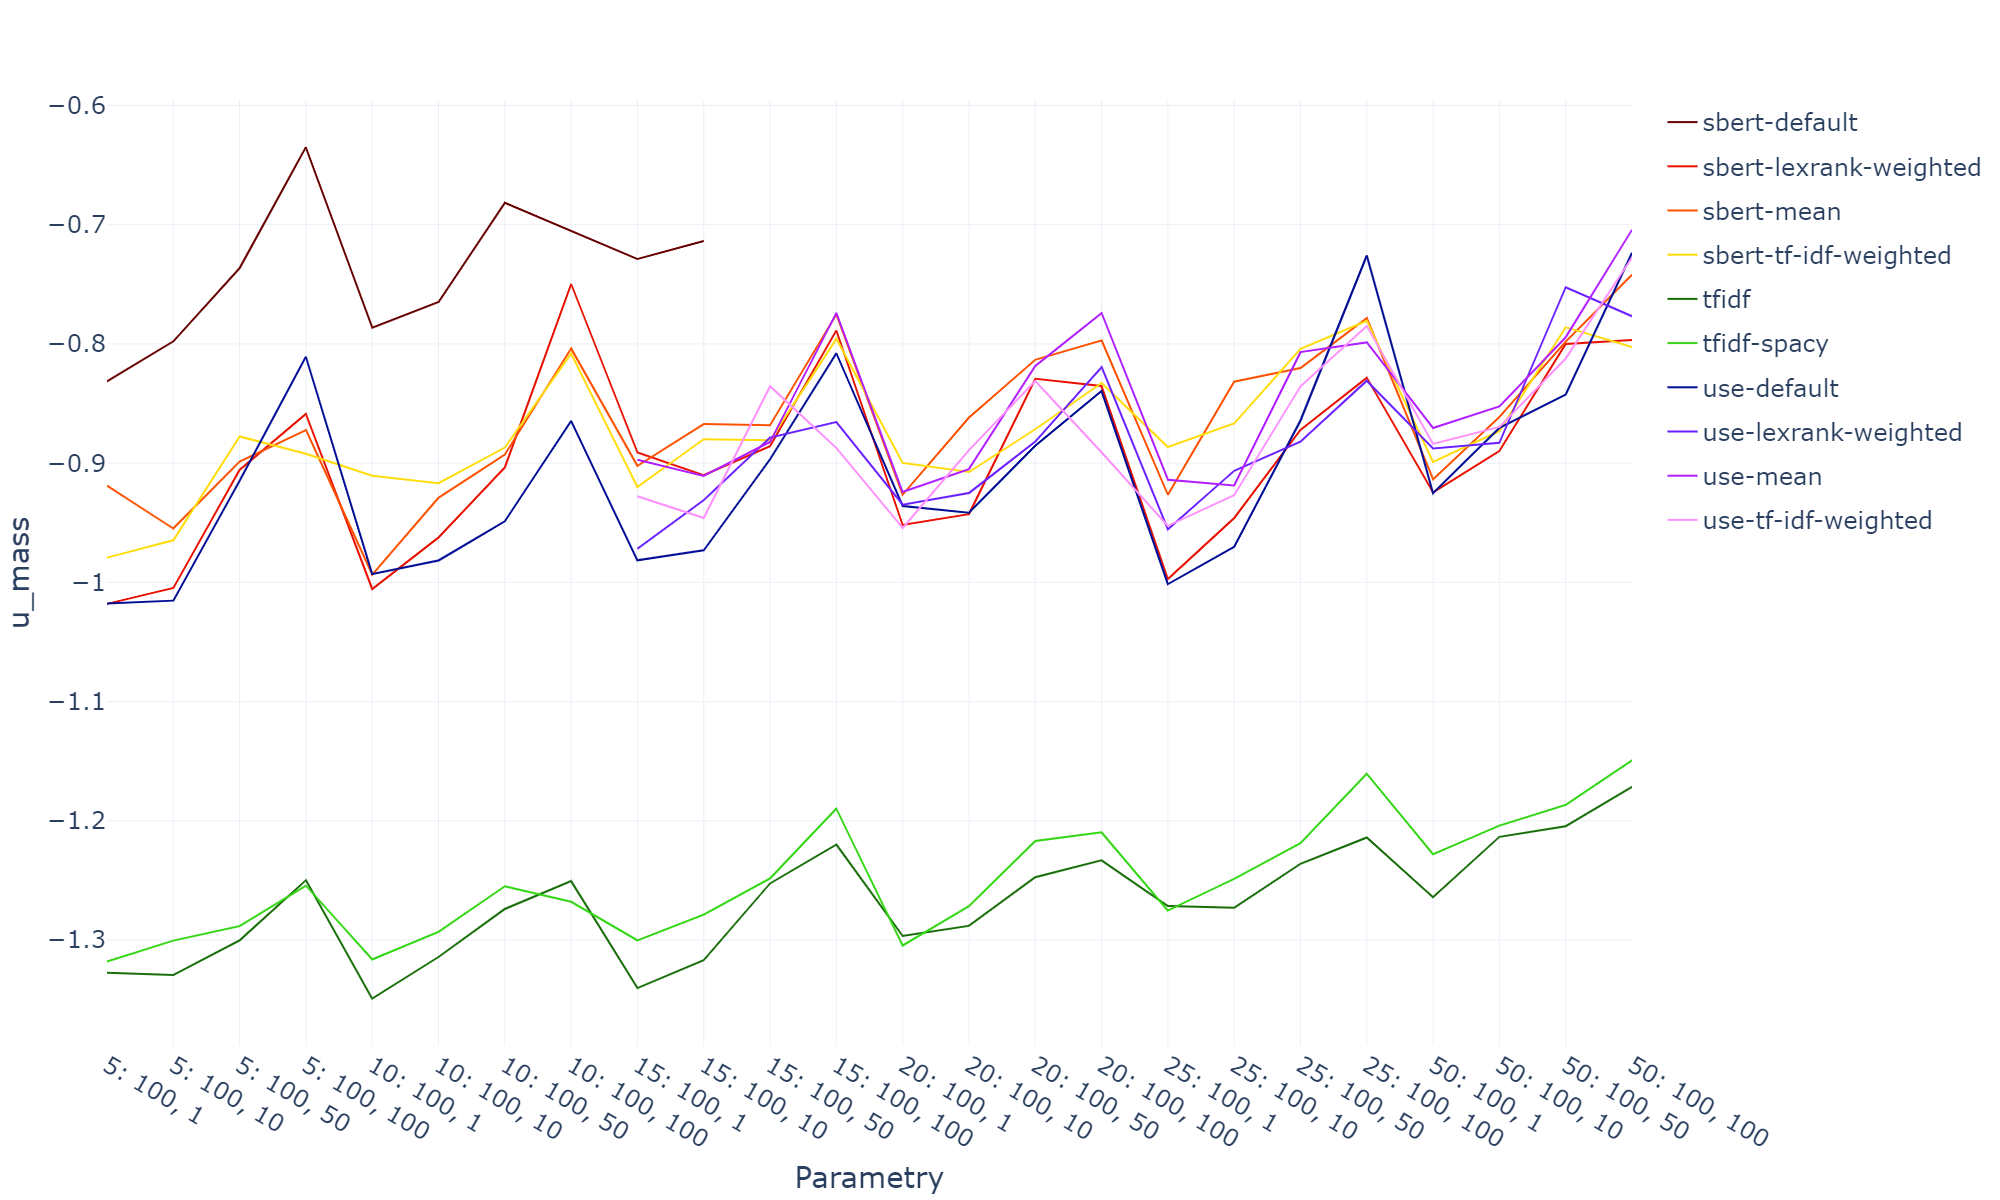
\includegraphics[width=\linewidth]{rys05/c_umass.png}
		\caption{Wyniki \(C_{UMass}\) dla parametru n\_neighbors równego 15}\label{fig:umass_score}
	\end{figure}

	Autorzy~\cite{C_NPMI} proponują rozwiązanie bazujące na wektorach kontekstowych słów tematu (zwane dalej \(C_{NPMI}\)).
	Wektory te są obliczane na podstawie współwystępujących słów w kontekście analizowanego słowa.
	Kontekst jest definiowany jako tzw.\ przesuwne okno (ang.\ \emph{sliding window}) zwierające \(\pm 5\) otaczających słów.
	Następnie wektory są ważone algorytmem NPMI (ang.\ \emph{Normalized Point Mutual Information}).
	Algorytm ten bazuje na PMI:
	\[PMI(w_i,w_j) = \log_2 \frac{p(w_i,w_j)}{p(w_i)p(w_j)}\]
	gdzie:
	\begin{itemize}
		\item \(p(w_i,w_j)\) prawdopodobieństwo współwystąpienia słów \(w_i\) i \(w_j\),
		\item \(p(w_i)\) prawdopodobieństwo wystąpienia słowa \(w_i\),
		\item \(p(w_j)\) prawdopodobieństwo wystąpienia \(w_j\).
	\end{itemize}
	Jeśli prawdopodobieństwo współwystąpienia dwóch słów jest takie samo, jak iloczyn prawdopodobieństw odlezienia każdego ze słów
		to znaczy że słowa nie są powiązane (ich współwystępowanie jest równe prawdopodobieństwu losowego odnalezienia tych dwóch słów).
	Wtedy wynik ułamka będzie równy 1, a \(\log(1)=0\), więc wartość PMI równa 0 oznacza, że słowa są niezależne.
	Wynik wyższy od 0 oznacza większe niż losowe prawdopodobieństwo odnalezienia danych dwóch słów razem,
		podczas gdy wartość poniżej zera oznacza prawdopodobieństwo niższe niż losowe (czyli częściej spotkamy tylko jedno ze słów, niż oba).

	Wariant NPMI normalizuje wynik PMI tak, aby mieścił się w zakresie [-1, 1]:
	\[NPMI(w_i,w_j) = \frac{PMI(w_i,w_j)}{-\log(p(w_i,w_j))}\]
	gdzie wartość 1 oznacza pełne współwystępowanie (\(p(w_i,w_j)=p(w_i)=p(w_j)\), czyli słowa nigdy nie występują osobno.
	Wartość -1 oznacza brak współwystępowania (słowa nigdy nie występują razem), a wartość 0 oznacza, że współwystępowanie słów jest losowe.

	Końcowa wartość obliczana jest jako średnia odległość kosinusowa między wszystkimi parami ważonych wektorów kontekstowych słów tematu.
	Wykres dla \emph{n\_neighbors} równego 15 przedstawiony został na rys.~\ref{fig:npmi_score}.

	\begin{figure}[htb]
		\centering
		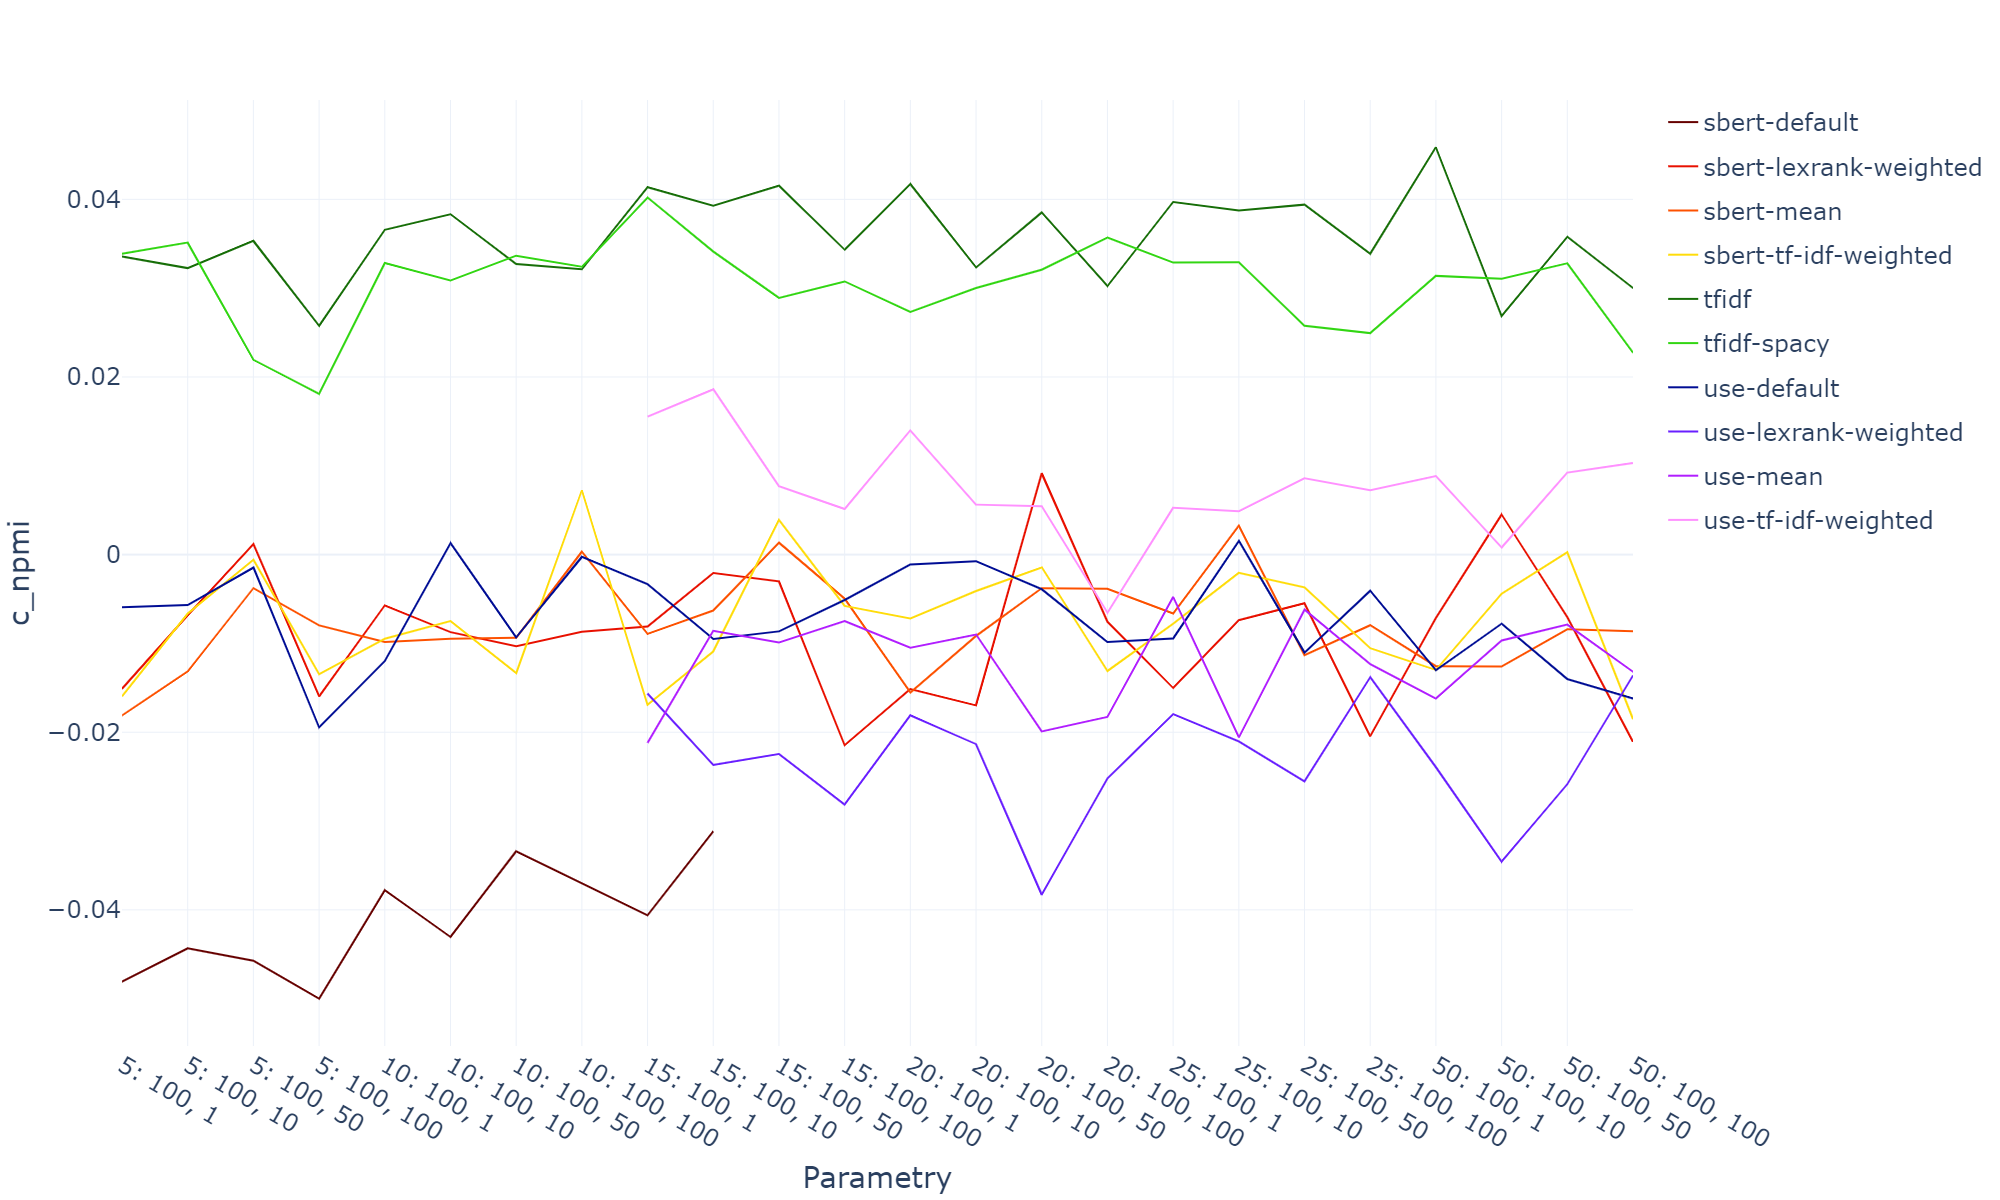
\includegraphics[width=\linewidth]{rys05/c_npmi.png}
		\caption{Wyniki \(C_{NPMI}\) dla parametru n\_neighbors równego 15}\label{fig:npmi_score}
	\end{figure}

	W pracy~\cite{Eval_Topics} autorzy stworzyli bazową strukturę pozwalającą na zdefiniowanie metryk \(C_{UMass}\), \(C_{NPMI}\)
		oraz innych miar spójności w jednej przestrzeni.
	W projekcie skorzystano z biblioteki \verb|Gensim|\footnote{\url{https://radimrehurek.com/gensim/models/coherencemodel.html} (dostęp dnia 29 maja 2021)},
		która implementuje miary spójności na podstawie tych definicji.

\section{Ewaluacja spójności rozkładu tematów}\label{sec:consistency_scores}
	Ze względu na specyfikę korpusu możliwe jest również sformułowanie metryki wykorzystującej porządek obrad sejmu.
	Każde posiedzenie przebiega zgodnie z ustaloną strukturą, gdzie marszałek zarządza obrady na temat danej ustawy, poprawki czy interpelacji,
		a następnie kolejni posłowie wyrażają swoją opinię na ten temat.
	Można więc założyć, że w obrębie debaty nad jednym punktem obrad, wypowiedzi powinny zostać zakwalifikowane do tego samego zbioru tematycznego.
	Stworzono więc algorytm wykorzystujący tę zależność, przedstawiony na listingu~\ref{lst:consistency_alg}.
	Implementacja algorytmu w języku Python pokazana jest na listingu~\ref{lst:score_consistency}.
	Założono, że w zdecydowanej większości przypadków, kolejne dwie wypowiedzi powinny mieć przypisany ten sam temat.

	Algorytm analizuje osobno każdy dzień posiedzeń.
	Wypowiedzi sortowane są zgodnie z kolejnością wynikającą z transkrypcji przemówień.
	Jeśli w ciągu dnia jest mniej niż dwie wypowiedzi, to dzień jest pomijany.
	W zbiorze danych występuje jeden taki przypadek, natomiast mediana wynosi 138.
	Wśród wypowiedzi danego dnia porównywane są tematy par sąsiadujących wypowiedzi.
	Zliczane są zarówno znalezione pasujące pary, jak i różniące się.
	Jeśli temat analizowanej wypowiedzi jest nieznany (algorytm HDBSCAN nie przypisał dokumentu do żadnej grupy),
		to jest ona pomijana.
	Mechanizm ten zapobiega sytuacji, w której duża liczba nieprzypisanych dokumentów zawyżałaby wynik.
	Dzieje się tak ze względu na to, że nieprzypisane dokumenty często stanowią znaczną część zbioru (30--50\%),
		przez co istnieje duże prawdopodobieństwo znalezienia par takich dokumentów.
	Dodatkowo, od sumy różniących się par odejmowana jest liczba o 1 mniejsza od liczby tematów danego dnia.
	Działanie to rekompensuje przejścia między tematami, które muszą wystąpić i nie są błędem.
	Takich przejść w ciągu dnia wystąpi co najmniej tyle, ile jest tematów minus jeden.
	Końcowy wynik obliczany jest jako stosunek zgadzających się par do wszystkich zliczonych par.

	Wykres dla parametru \emph{min\_cluter\_size} równego 100 przedstawiony został na wykresie~\ref{fig:consistency_score}.
	
	\begin{lstlisting}[style=algorithm,label=lst:consistency_alg,caption=Algorytm obliczania spójności tematów]
input: speeches sorted by original order of speaking, with date and assigned topic identifier
output: consistency score between 0 and 1 with higher score indicating more consistent topics
	
same_per_day := []
different_per_day := []

for each speeches in data grouped by date do
	if len(speeches) < 2
		continue
	
	same := 0
	different := 0
	for i in range(len(speeches) - 1) do
		if speeches[i].topic is unknown
			continue

		if speeches[i].topic = speeches[i + 1].topic
			same := same + 1
		else
			different := different + 1

	topic_count := len(speeches.topic.unique())
	different := different - (topic_count - 1)
	
	same_per_day.append(same)
	different_per_day.append(different)

score = sum(same_per_day) / sum(same_per_day, different_per_day)
return score
	\end{lstlisting}

	\begin{figure}[htb]
		\centering
		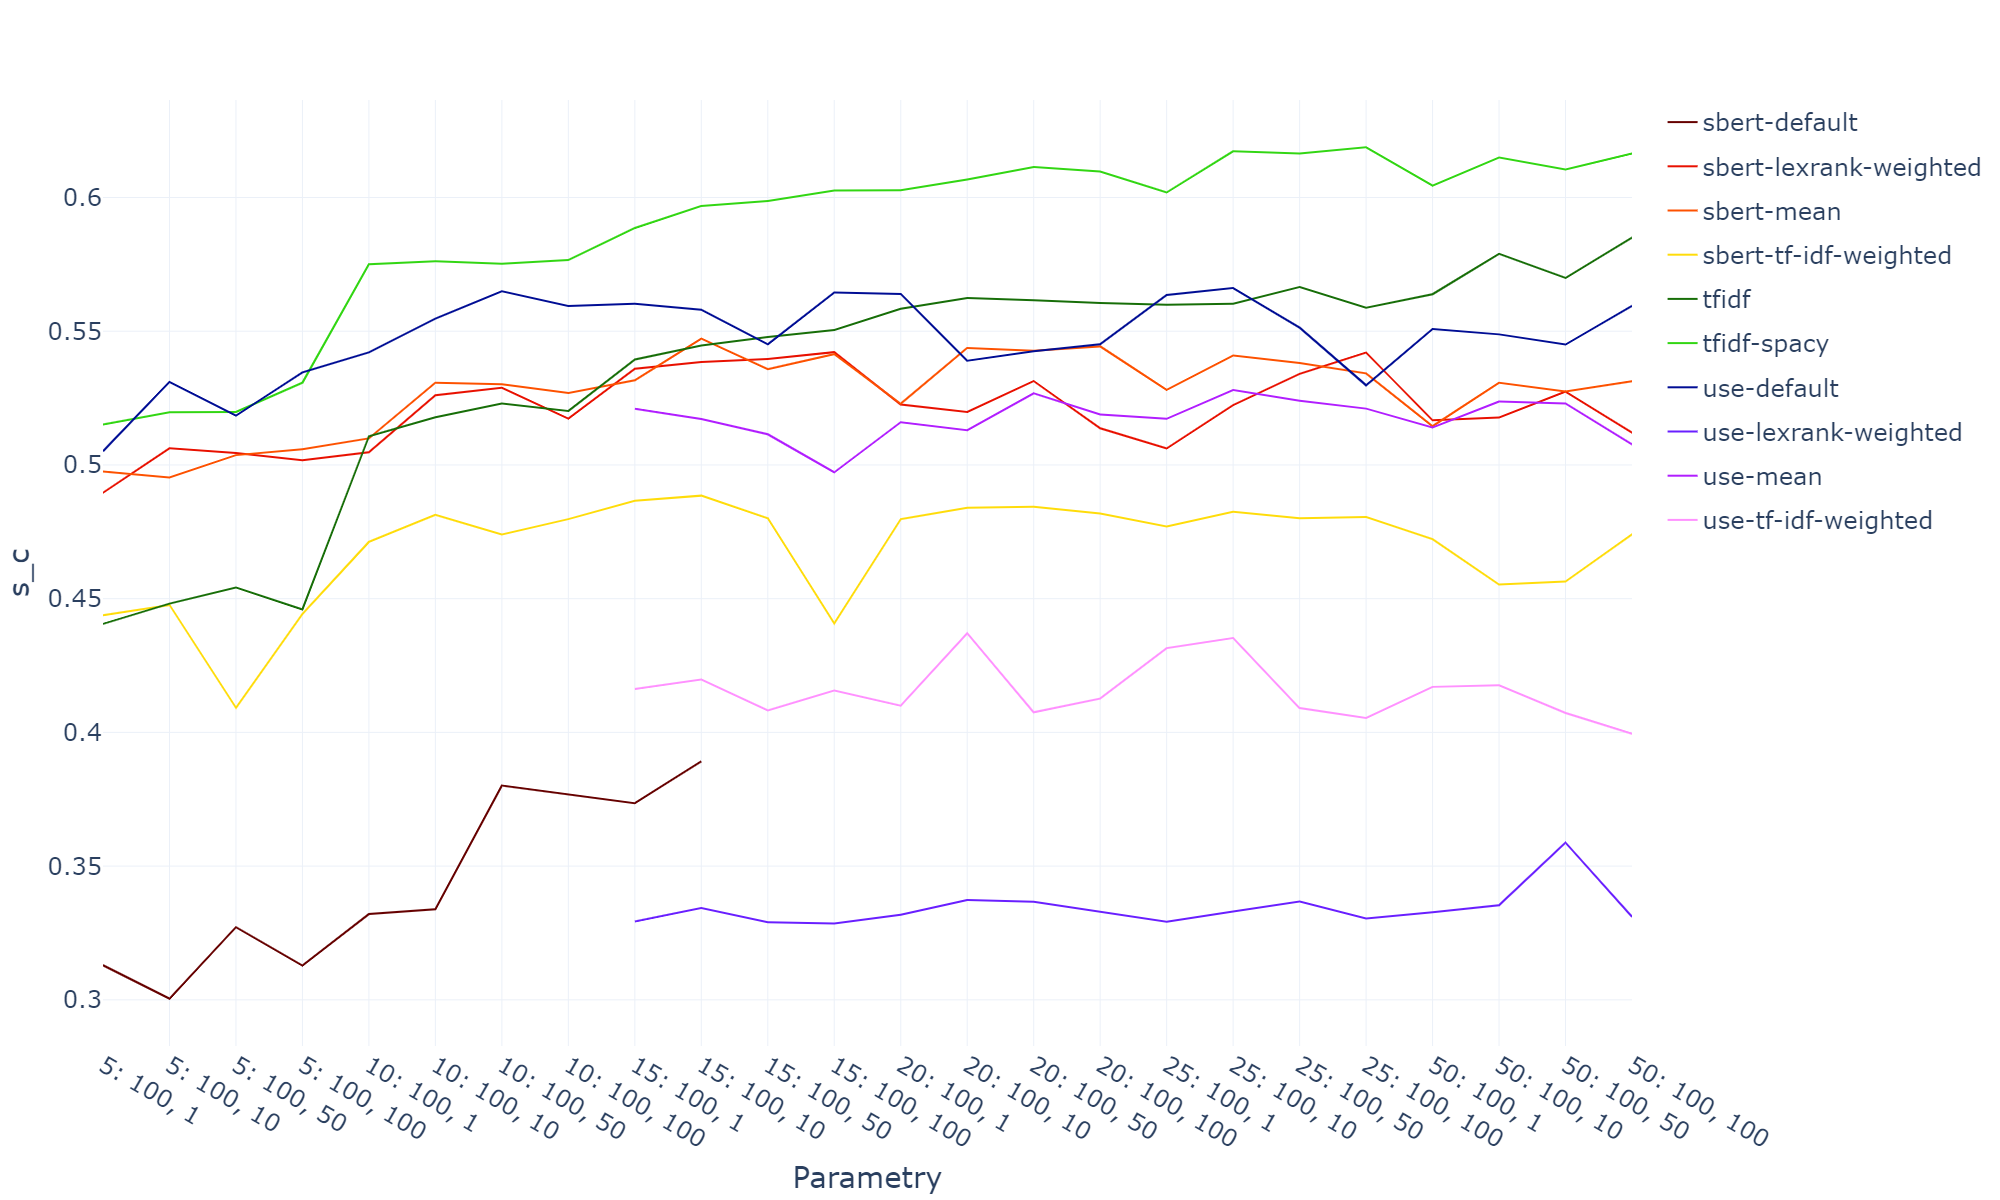
\includegraphics[width=\linewidth]{rys05/s_c.png}
		\caption{Wyniki \(s_c\) dla parametru \emph{min\_cluster\_size} równego 100}\label{fig:consistency_score}
	\end{figure}

\section{Końcowa ocena}
	Powyższe metody nie poddają ocenie samej liczby tematów i liczby nieprzyporządkowanych dokumentów.
	Z tego powodu, wysoki wynik mógłby osiągnąć model, który znalazłby zaledwie 5 tematów.
	Takie przypadki można znaleźć w tabeli z wynikami (rozdział~\ref{sec:all_scores}) dla modeli \emph{sbert-default}.
	Taki model przyporządkuje wszystkie dokumenty generując bardzo ogólne tematy.
	Podobnie wysoki wynik osiągnie model, który wygeneruje tysiące bardzo szczegółowych tematów.
	Takie modele można odfiltrować definiując odpowiednie progi, jednak taka metoda wymusza ustanowienie założeń,
		które niekoniecznie będą optymalne.
	Zamiast tego, stworzone zostały dwie dodatkowe miary: jedna ocenia liczbę przyporządkowanych dokumentów \(s_f\), druga ocenia liczbę tematów \(s_T\).
	Końcowa ocena modelu jest średnią ocen \(C_{UMass}\), \(C_{NPMI}\), \(s_c\), \(s_f\) oraz \(s_T\) przeskalowanych do pełnego zakresu (0, 1).
	Skalowanie odbywa się przy pomocy klasy \verb|MinMaxScaler| z biblioteki \verb|scikit-learn|,
		jak przedstawiono w linijce 18 listingu~\ref{lst:final_score}.
	Wykres końcowej, uśrednionej oceny dla każdego parametru przedstawiony jest na rysunku~\ref{fig:avg_scores}.

	\begin{figure}
		\centering
		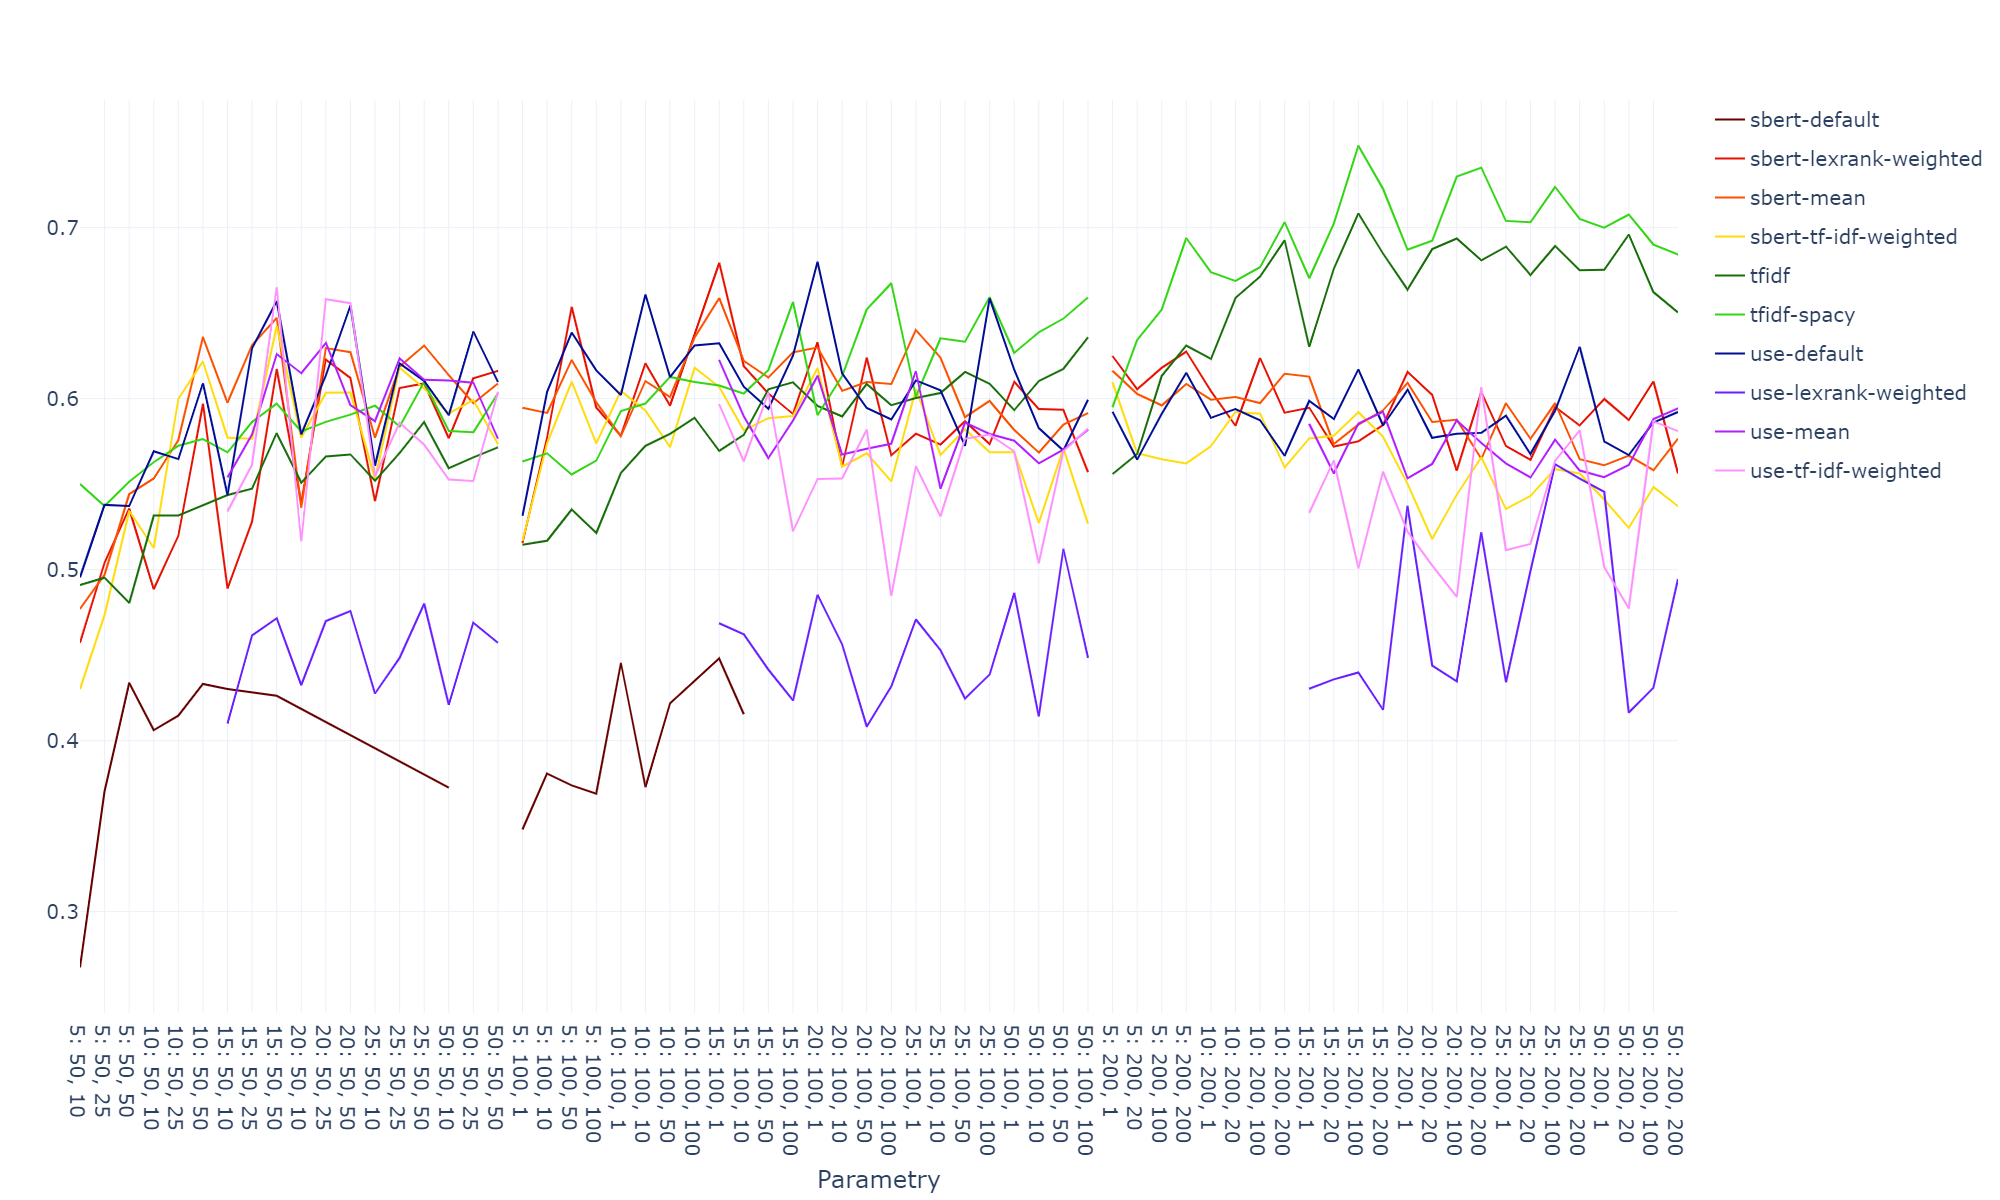
\includegraphics[width=1.5\textwidth,angle=90]{rys05/avg.png}
		\caption{Uśrednione wyniki dla parametrów \(min\_cluster\_size\in \left[50, 100, 200\right]\)}\label{fig:avg_scores} % chktex 35
	\end{figure}

	\subsection{Ocena liczby przyporządkowanych dokumentów}\label{sec:score_not_found}
		Miara oceniająca liczbę przyporządkowanych dokumentów korzysta bezpośrednio z wyniku grupowania.
		Grupa oznaczona jako '-1' oznacza dokumenty, które nie zostały zgrupowane, a więc nie mają przypisanego tematu.
		Rozmiar tej grupy odejmowany jest od rozmiaru korpusu uzyskując liczbę dokumentów z rozpoznanymi tematami.
		Liczba ta dzielona jest przez rozmiar korpusu, co daje miarę w przedziale (0, 1).
		Działanie to przedstawione jest w linijce 16 listingu~\ref{lst:final_score},
			gdzie \verb|scores['not_found']| to kolumna tabeli zawierająca rozmiar grupy nieprzyporządkowanych dokumentów dla każdego modelu.
		
		Przykładowy wynik działania tej metody przedstawiony został na rysunku~\ref{fig:not_found}.

		\begin{figure}[htb]
			\centering
			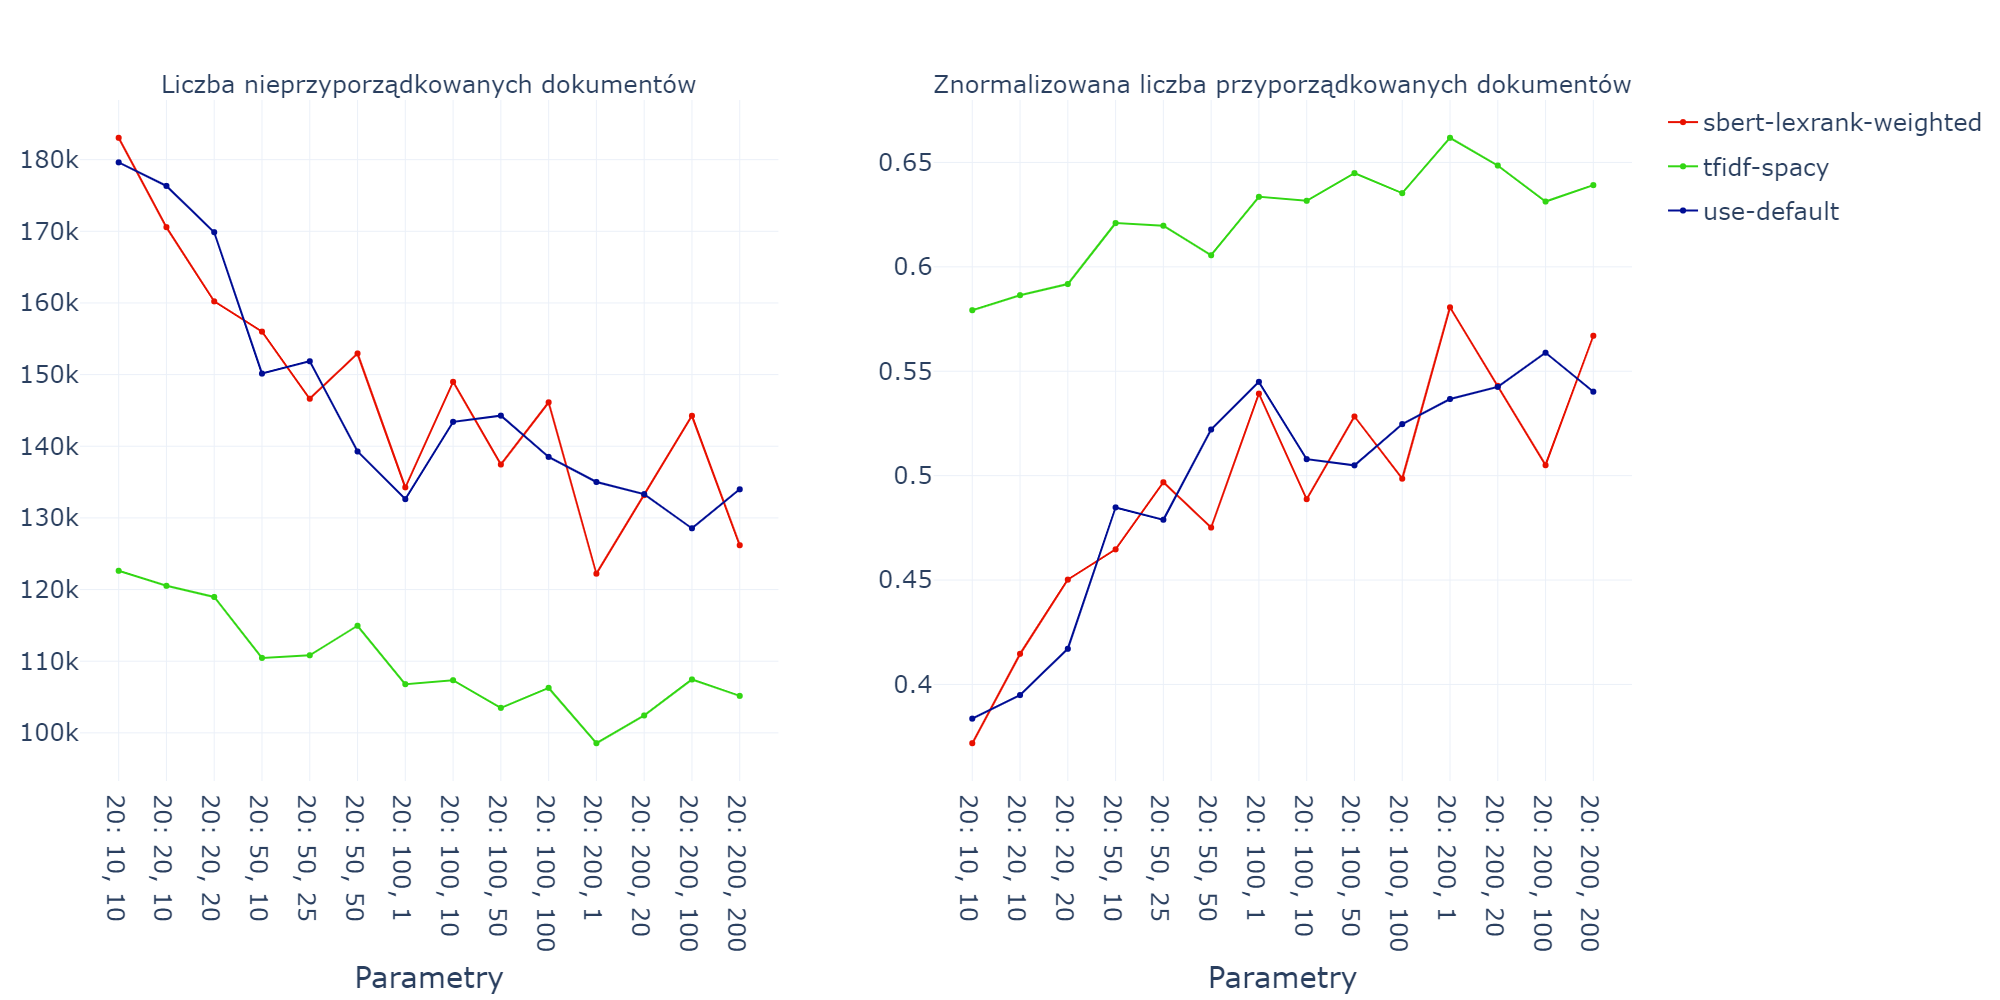
\includegraphics[width=\linewidth]{rys05/not_found.png}
			\caption{Liczba rozpoznanych dokumentów przed i po znormalizowaniu dla wybranych parametrów}\label{fig:not_found}
		\end{figure}

	\subsection{Ocena liczby tematów}\label{sec:score_topic_count}
		Dużo trudniej jest ocenić liczbę tematów, gdyż zarówno osiemdziesiąt ogólnych tematów,
			jak i tysiąc szczegółowych mogą zostać uznane za odpowiednie.
		Zważając jednak na specyfikę korpusu, przyjęto że różnorodność poruszanych kwestii powinna skutkować relatywnie dużą liczbą tematów.
		Z tego powodu uznano, że zbyt ogólne tematy nie są odpowiednie w tym kontekście.
		Nadmiernie szczegółowe, a więc o małej liczebności tematy również tracą informacje o zależnościach między dokumentami,
			więc także uznane zostały za niepożądane.
		W takim wypadku za odpowiednią liczbę tematów przyjęto medianę liczby tematów dla wszystkich testowanych modeli, która wyniosła 219.

		W celu określenia wyniku każdego modelu wykorzystano zmodyfikowaną standaryzację Z.
		Standaryzacja Z obliczana jest zgodnie z następującym wzorem:
		\[z=\frac{x-\mu}{\sigma}\]
		gdzie:
		\begin{itemize}
			\item \(x\) wartość zmiennej,
			\item \(\mu\) średnia z populacji,
			\item \(\sigma\) odchylenie standardowe populacji.
		\end{itemize}
		
		Średnia arytmetyczna i odchylenie standardowe są jednak podatne na wpływ wartości leżących daleko od średniej.
		Z tego powodu często wykorzystywana jest zmodyfikowana standaryzacja Z, która mierzy odległości od mediany:
		\[\tilde{z}=\frac{x-\tilde{x}}{k\cdot MAD}\]
		gdzie:
		\begin{itemize}
			\item \(x\) wartość zmiennej,
			\item \(\tilde{x}\) mediana z populacji,
			\item \(k=1.486\) wartość korekcyjna stanowiąca przybliżenie odchylenia standardowego,
			\item \(MAD\) średnie odchylenie bezwzględne --- \(median\left(|x_i-\tilde{x}|\right)\).
		\end{itemize}

		Tak ustandaryzowane dane rozłożone są wokół zera, gdzie liczby tematów mniejsze od mediany mają ujemny wynik, a większe dodatni.
		Takie odległości interpretowane są jako odległości od najlepszej liczby tematów,
			im większa odległość tym gorszy powinien być wynik takiego modelu.
		W celu dodatkowego ograniczenia wpływu pomiarów zwracających błędną liczbę tematów, medianę obliczono dla ograniczonego zakresu (50, 1000).
		Aby wyrazić te odległości w skali (0, 1), gdzie 1 to najlepszy wynik, znormalizowano dane
			poprzez odwrócenie wartości bezwzględnej standaryzacji Z powiększonej o 1 (aby minimalna wartość była równa 1):
		\[s_T=\frac{1}{|\tilde{z}|+1}\]
		Implementacja tej miary przedstawiona została na listingu~\ref{lst:final_score} jako funkcja \verb|modified_zscore|.
		Wykres liczby tematów dla wybranego fragmentu parametrów przed i po znormalizowaniu przedstawiony został na rysunku~\ref{fig:topic_counts}.

		\begin{figure}[htb]
			\centering
			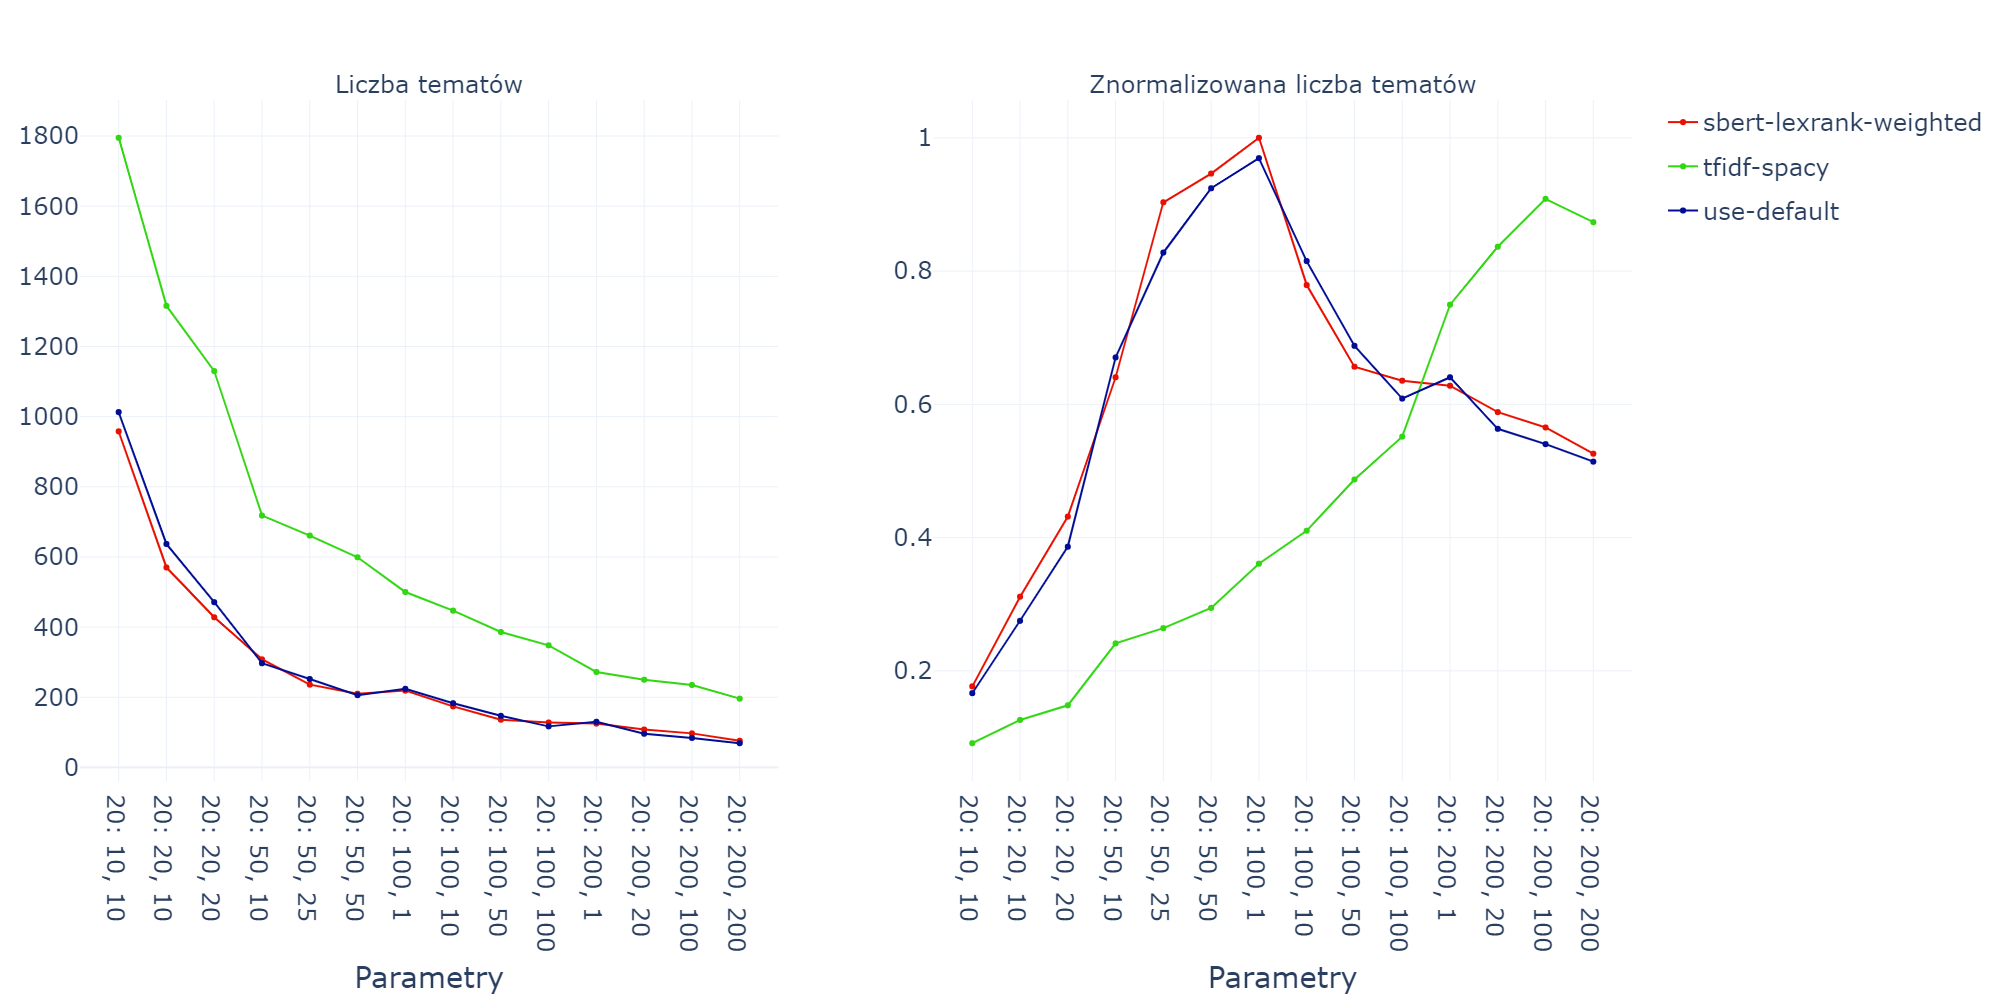
\includegraphics[width=\linewidth]{rys05/topic_counts.png}
			\caption{Liczba tematów przed i po znormalizowaniu dla wybranych parametrów}\label{fig:topic_counts}
		\end{figure}

	\subsection{Implementacja}
		Algorytmy zaimplementowane zostały w języku Python.
		Wykorzystane zostały biblioteki \verb|numpy|, \verb|pandas|, \verb|scikit-learn| oraz \verb|scipy|.

		\begin{lstlisting}[label=lst:score_consistency,language=Python,caption=Funkcja obliczająca spójność s\_c]
def score_consistency(df: pd.DataFrame) -> float:
	same_per_day = []
	different_per_day = []

	for _, day in df.sort_values('speech_order').groupby(by='date'):
		if len(day) < 2:
			continue

		same = 0
		different = 0
		for i in range(len(day) - 1):
			if day.iloc[i].topic == -1:
				continue

			if day.iloc[i].topic == day.iloc[i + 1].topic:
				same += 1
			else:
				different += 1

		topics = len(day.topic.unique())
		different -= (topics - 1)

		same_per_day.append(same)
		different_per_day.append(different)

	s_c = np.sum(same_per_day) / np.sum([*same_per_day, *different_per_day])

	return s_c
		\end{lstlisting}

		\begin{lstlisting}[label=lst:final_score,language=Python,caption=Obliczanie finalnej oceny spójności tematów dla listy modeli]
from sklearn.preprocessing import MinMaxScaler
from scipy import stats
import numpy as np

def modified_zscore(x: List[float]) -> List[float]:
	valid_x = [count for count in x if count > 50 and count < 1000]
	median = np.median(valid_x)
	deviation_from_med = x - median

	mad = np.median(np.abs(deviation_from_med))

	consistency_correction = 1.4826
	mod_zscore = deviation_from_med / (consistency_correction * mad)

	return mod_zscore

scores['s_f'] = [(total - x) / total for x in scores['not_found']]

scores['s_T'] = 1 / (np.abs(modified_zscore(scores['topic_count'])) + 1)

scaler = MinMaxScaler()
s = scaler.fit_transform(scores[['u_mass','c_npmi','s_c','s_f','s_T']])

scores['avg'] = np.nanmean(s, axis=1)
		\end{lstlisting}

\section{Przeprowadzenie pomiarów}\label{sec:test_plan}
	Pomiary metodami opisanymi w poprzednim rozdziale zaplanowano tak, by wyniki umożliwiły jak najszerszą analizę porównawczą.
	Wektory zdań generowano następującymi metodami opisanymi w rozdziale~\ref{sec:vectors}:
	\begin{itemize}
		\item Sentence-Transformers,
		\item Universal Sentence Encoder,
		\item TF-IDF\@.
	\end{itemize}
	Dodatkowo, dla pierwszych dwóch metod wykonano pomiary dla następujących sposobów łączenia wektorów zdań w wektory wypowiedzi (rozdział~\ref{sec:sentences}):
	\begin{itemize}
		\item LexRank (top1, top5, średnia ważona),
		\item TF-IDF (top1, top5, średnia ważona),
		\item średnia arytmetyczna,
	\end{itemize}
	oraz bez podziału na zdania (generowanie wektora bezpośrednio dla całej wypowiedzi).
	Dla wektorów tf-idf przygotowano dwa warianty: jeden analizujący nieprzetworzone dokumenty
		oraz drugi wykorzystujący dane przetworzone w sposób opisany w rozdziale~\ref{sec:tfidf_vectors}.

	Redukcję wektorów wykonywano do pięciu wymiarów metryką kosinusową dla wektorów \emph{SBERT} i \emph{USE} oraz metryką Hellingera dla wektorów \emph{TF-IDF}.
	Zmieniano jedynie parametr \verb|n_neighbors| testując następujące wartości: 5, 10, 15, 20, 25 oraz 50, gdzie najmniejsze wartości skupiają się na lokalnych zależnościach,
		a większe wykrywają globalne struktury.
	Podczas klastrowania algorytmem HDBSCAN testowane były parametry \verb|min_cluster_size| oraz \verb|min_samples| w kombinacjach przedstawionych w tabeli~\ref{tab:hdbscan_params}.

	\begin{table}[htb]
		\caption{Testowane parametry algorytmu HDBSCAN}\label{tab:hdbscan_params}
		\centering
		\begin{tabular}{lrrrrrrrrrrrrrr}
			\toprule
			min\_cluster\_size	& 10 & \multicolumn{2}{l}{20} &  \multicolumn{3}{l}{50} & \multicolumn{4}{l}{100}	&  \multicolumn{4}{l}{200} \\
			min\_samples 				& 10 &  10 &  20 							&  10 &  25 &  50 				& 	1 &	10 &	50 &  100		&   1 &   20 &  100 &  200 \\
			\bottomrule
		\end{tabular}
	\end{table}

	Ze względu na złożoność obliczeniową pomiarów, w pierwszej kolejności przeprowadzono pomiary na ograniczonym zakresie:
	\begin{itemize}
		\item \verb|n_neighbors|: 5, 10, 15, 20
		\item \verb|min_cluster_size|: 10, 20, 50, 100
	\end{itemize}
	oraz pominięto liczenie wyniku \(C_{NPMI}\).
	W tabeli~\ref{tab:avg_scores}a przedstawiono posortowane, uśrednione wyniki \(C_{UMass}\), \(s_c\), \(s_f\) oraz \(s_T\).
	Na podstawie tych wyników zdecydowano się odrzucić metody bazujące na najlepszych wektorach wg.\ rankingu (top1 i top5),
		ponieważ zarówno dla algorytmu LexRank, jak i TF-IDF dawały one zauważalnie gorsze wyniki od pozostałych metod.
	Z tego powodu nie zostały one uwzględnione podczas obliczania wyników dla pełnego zakresu parametrów.
	Uśrednione wyniki na pełnym zakresie, uwzględniające również metodę \(C_{NPMI}\), przedstawione zostały w tabeli~\ref{tab:avg_scores}b.
	Dalsze omówienie tych wyników zawarte jest w kolejnym rozdziale.
		
	\begin{table}[htb]
		\caption{Średnie wyniki dla zakresu parametrów: a) ograniczonego, b) pełnego}\label{tab:avg_scores} % chktex 9 chktex 10
		\centering
		\begin{minipage}[t]{.5\textwidth}
			a)\par\medskip % chktex 10
			\begin{tabular}{lr}
				\toprule
								metoda &	średni wynik \\
				\midrule
								sbert-default & 0.412 \\
						sbert-tf-idf-top1 & 0.416 \\
							use-lexrank-top5 & 0.459 \\
						sbert-lexrank-top1 & 0.463 \\
					use-lexrank-weighted & 0.465 \\
							use-lexrank-top1 & 0.489 \\
							use-tf-idf-top5 & 0.501 \\
						sbert-tf-idf-top5 & 0.505 \\
												tfidf & 0.516 \\
					use-tf-idf-weighted & 0.522 \\
						sbert-lexrank-top5 & 0.523 \\
									tfidf-spacy & 0.558 \\
											use-mean & 0.559 \\
				sbert-tf-idf-weighted & 0.565 \\
				sbert-lexrank-weighted & 0.572 \\
										sbert-mean & 0.587 \\
									use-default & 0.593 \\
				\bottomrule
			\end{tabular}
		\end{minipage}%
		\begin{minipage}[t]{.5\textwidth}
			b)\par\medskip % chktex 10
			\begin{tabular}{lr}
				\toprule
								metoda &	średni wynik \\
				\midrule
								sbert-default & 0.331 \\
					use-lexrank-weighted & 0.426 \\
					use-tf-idf-weighted & 0.525 \\
				sbert-tf-idf-weighted & 0.531 \\
				sbert-lexrank-weighted & 0.545 \\
											use-mean & 0.551 \\
										sbert-mean & 0.557 \\
									use-default & 0.558 \\
												tfidf & 0.580 \\
									tfidf-spacy & 0.617 \\
				\bottomrule
				\end{tabular}
		\end{minipage}
	\end{table}

	\subsection{Optymalizacje}
		Ze względu na złożoność pamięciową algorytmów badających spójność reprezentacji tematów (rozdział~\ref{sec:coherence_scores}),
			algorytmy te badały ograniczony zbiór dokumentów.
		Aby jednak zachować zależności między dokumentami na pełnym zbiorze, w pierwszym kroku algorytm HDBSCAN grupuje wszystkie dokumenty.
		Dopiero z pogrupowanych dokumentów losowane są próbki według zdefiniowanych \(test\_sample\) oraz \(test\_sample\_frac\),
			które odpowiednio oznaczają minimalną liczbę próbek z każdej grupy, oraz część grupy.
		Próbki losowane są w zależności od rozmiaru grupy \(N\):
		\begin{itemize}
			\item jeśli \(N\) jest większe niż \(\frac{test\_sample}{test\_sample\_frac}\), to losujemy \(test\_sample\_frac \cdot N\) próbek,
			\item jeśli \(N\) jest większe niż \(test\_sample\), to losujemy \(test\_sample\) próbek,
			\item jeśli \(N\) jest mniejsze niż \(test\_sample\), to bierzemy wszystkie \(N\) próbek.
		\end{itemize}
		Ustawiając \(test\_sample=100\) oraz \(test\_sample\_frac=0.2\) sprawiono,
			że brane pod uwagę jest 20\% dokumentów z każdej grupy, ale nie mniej niż 100 (lub całość grupy).
		Dolne ograniczenie \(test\_sample\) sprawia, że nie zawsze analizowane jest tyle samo dokumentów.
		W zależności od liczby wykrytych tematów, analizowanych jest średnio od 60 do 90 tysięcy próbek (tabela~\ref{tab:support}).
		Dodatkowo, jeśli liczba odnalezionych tematów była mniejsza niż 20 lub większa niż 1000, to testy \(C_{NPMI}\) oraz \(C_{UMass}\) były pomijane.

		Przeprowadzenie klastrowania na pełnym zbiorze danych umożliwia również poprawne przeprowadzenie testów spójności rozkładów tematów (rozdział~\ref{sec:consistency_scores})
			na wszystkich dokumentach, co jest wymogiem algorytmu (ponieważ potrzebujemy wszystkie pary występujące zaraz po sobie).
		Oceny liczby przyporządkowanych dokumentów oraz liczby tematów opisane odpowiednio w rozdziałach~\ref{sec:score_not_found},~\ref{sec:score_topic_count}
			również przeprowadzone zostały na pełnym korpusie.

		\begin{table}[htb]
			\caption{Liczba analizowanych próbek w zależności od liczby wykrytych tematów (mediana)}\label{tab:support}
			\centering
			\begin{tabular}{lrl}
				\toprule
				liczba tematów  &  liczba próbek	&	\% korpusu \\
				\midrule
				(4 74]     &  58652 &	20.1\% \\
				(74 107]   &  59586 &	20.4\% \\
				(107 136]  &  61376 &	21.1\% \\
				(136 175]  &  63410 &	21.8\% \\
				(175 216]  &  65728 &	22.6\% \\
				(216 260]  &  67814 &	23.3\% \\
				(260 363]  &  70716 &	24.3\% \\
				(363 502]  &  75451 &	25.9\% \\
				(502 791]  &  82544 &	28.3\% \\
				(791 3166] &  92502 &	31.7\% \\
				\bottomrule
			\end{tabular}
		\end{table}

\section{Ewaluacja LDA}\label{sec:lda}
	Tematy uzyskane metodą BERTopic zostały porównane z popularną metodą analizy tematycznej --- LDA\@.
	W tym celu wykonano pomiary spójności algorytmami opisanymi w poprzednich rozdziałach.
	Jedną z zasadniczych wad algorytmu LDA jest fakt, iż liczba tematów jest jego parametrem.
	Aby znaleźć optymalną liczbę tematów, przeprowadzono pomiary dla różnych wartości parametru z zakresu [10--300].
	Dokumenty przetworzono tą samą metodą, co w przypadku generowania wektorów TF-IDF w rozdziale~\ref{sec:tfidf_vectors},
		mianowicie lematyzacja słownikami \emph{Morfeusz2}, usunięcie polskich słów bez znaczenia (ang.\ \emph{stop words}) oraz wygenerowanie bigramów.
	Ze względu na ograniczenia techniczne związane z pamięcią operacyjną maszyny (128GB), analizie poddano sto tysięcy losowo wybranych dokumentów,
		co stanowi ok.~34\% całości korpusu.
	Wyniki tych pomiarów przedstawione są na rysunku~\ref{fig:lda_scores} oraz w tabeli~\ref{tab:lda_scores}.
	Z danych można odczytać, że dokładność modelu utrzymuje się na podobnym poziomie do ok.~80 tematów, potem zaczyna gwałtownie spadać.
	Za optymalną liczbę tematów wybrano więc 80 ze względu na zróżnicowanie korpusu, który z pewnością zawiera dużo tematów.

	\begin{figure}[htb]
		\centering
		\begin{minipage}{.5\textwidth}
			a)\par\medskip % chktex 10
			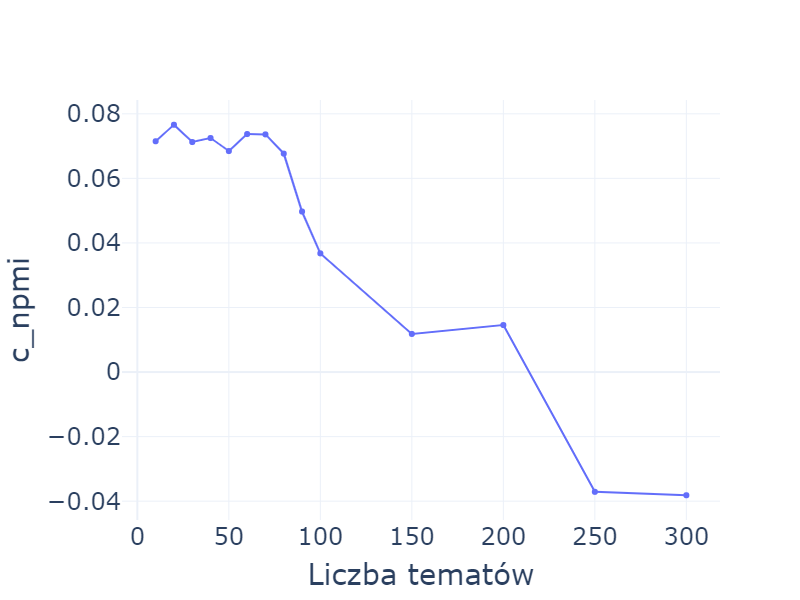
\includegraphics[width=\linewidth]{rys05/lda_c_npmi.png}
		\end{minipage}%
		\begin{minipage}{.5\textwidth}
			b)\par\medskip % chktex 10
			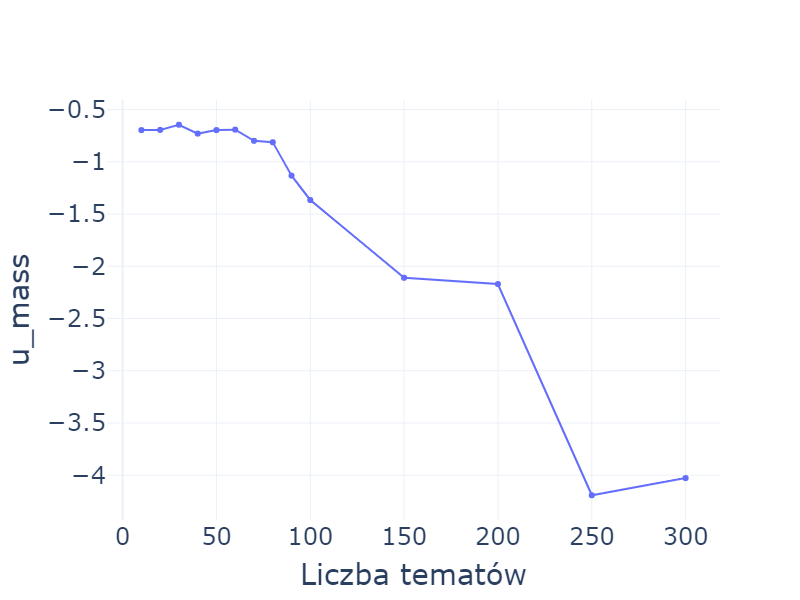
\includegraphics[width=\linewidth]{rys05/lda_u_mass.png}
		\end{minipage}
		\caption{Wyniki pomiarów dla LDA:\ a) \(C_{NPMI}\), b) \(C_{UMass}\)}\label{fig:lda_scores} % chktex 9 chktex 10
	\end{figure}

	\begin{table}[htb]
		\centering
		\caption{Wyniki pomiarów dla LDA w zależności od liczby tematów}\label{tab:lda_scores}
		\begin{tabular}{lrr}
			\toprule
			{} &    c\_npmi &    u\_mass \\
			\midrule
			10  &  0.071499 & -0.696868 \\
			20  &  0.076610 & -0.694938 \\
			30  &  0.071255 & -0.645520 \\
			40  &  0.072496 & -0.730301 \\
			50  &  0.068460 & -0.696550 \\
			60  &  0.073730 & -0.692332 \\
			70  &  0.073619 & -0.799463 \\
			80  &  0.067665 & -0.813064 \\
			90  &  0.049716 & -1.132477 \\
			100 &  0.036761 & -1.366198 \\
			150 &  0.011804 & -2.110305 \\
			200 &  0.014556 & -2.170508 \\
			250 & -0.037109 & -4.191849 \\
			300 & -0.038166 & -4.027447 \\
			\bottomrule
		\end{tabular}
	\end{table}

	Dla znalezionych tematów wygenerowano reprezentacje składające się z pięciu najwyżej ocenianych słów.
	Losowo wybrane 5 tematów przedstawiono w tabeli~\ref{tab:lda_topics}a.
	Dodatkowo, ze względu na to, iż mediana liczby znalezionych tematów algorytmem HDBSCAN wyniosła 219,
		postanowiono zbadać również model LDA dla 200 tematów (tabela~\ref{tab:lda_topics}b).
	Dla obu tych modeli widoczny jest problem opisany na początku rozdziału~\ref{sec:topic_modeling}.
	Mianowicie, reprezentacje tematów zawierają wiele podobnych słów specyficznych dla całego korpusu, a nie tematu (,,ustawa'', ,,minister'', czy ,,poseł'').
	Podjęto próby poszerzenia listy słów nieinformatywnych, jednak szybko okazało się, iż takich słów jest zbyt wiele
		--- po usunięciu słów specyficznych dla korpusu nadal reprezentacje tematów składały się często ze słów typu ,,czas'', ,,kwestia'', ,,chodzi''.
	Nie stwierdzono zauważalnej różnicy między dokładnością reprezentacji wygenerowanych dla 80 tematów, a tymi dla 200.
	Niezadowalająca skuteczność LDA na używanym korpusie może być związana ze specyfiką posiedzeń sejmowych.
	Stenografy z przemówień często zawierają różne komentarze, odniesienia do poprzedzających wypowiedzi itp.
	W momencie, kiedy mówca wypowiada się jedynie nawiązując do tematu słowami typu ,,proponowana ustawa'',
		nie sposób zrozumieć, o czym jest mowa, bez analizy poprzedzających wypowiedzi.
	Jedną z zalet algorytmu HDBSCAN jest wykrywanie szumu, a więc takie wypowiedzi nie są na siłę przyporządkowywane do jakiegoś jednego tematu.
	Dzięki temu tematy są znacznie bardziej spójne, niż te wygenerowane przez LDA\@.

	\begin{table}[htb]
		\caption{Reprezentacje pięciu losowo wybranych tematów dla LDA:\ a) 80 tematów, b) 200 tematów}\label{tab:lda_topics} % chktex 9 chktex 10
		\centering
		a) % chktex 10
		\begin{tabularx}{.7\textwidth}{rl}
			\toprule
			A	&	rok | mieć | europejski | minister | r	\\ 
			B	&	państwo | ustawa | mieć | rok | Polska	\\ 
			C	&	minister | państwo | dziecko | rok | szkoła	\\
			D	& minister | poseł | pytanie | mieć | chcieć	\\
			E	& ustawa | mieć | poseł | wysoki | poprawka	\\
			\midrule
		\end{tabularx}

		b) % chktex 10
		\begin{tabularx}{.7\textwidth}{rl}
			A	&	ustawa | projekt | ustawy | komisja | wysoki	\\ 
			B	&	rok | mieć | minister | poseł | Maryja \\ 
			C	&	ustawa | zmiana | projekt | prawo | ustawy \\
			D	&	trybunał | konstytucyjny | ustawa | rok | Trybunału	\\
			E	&	ustawa | mieć | rok | Pan | sprawa	\\
			\bottomrule
		\end{tabularx}
	\end{table}

% !TeX root = ./Dyplom.tex

\chapter{Analiza wyników}
	Szczegółowe wyniki zostały przedstawione w rozdziale~\ref{sec:all_scores}.
	W tabeli zawarte są wszystkie metody, dla których wykonane zostały pełne testy (jak opisano w rozdziale~\ref{sec:test_plan}).
	W kolumnach przedstawiono kolejno parametry testów, liczbę znalezionych tematów i liczbę nieprzypisanych dokumentów, wyniki testów oraz wynik uśredniony.
	Jeśli dla danych parametrów liczba tematów była poza zakresem [50--1000], to niektóre testy były pomijane w celach optymalizacyjnych.
	Wtedy w kolumnach wpisana jest wartość ,,<NA>''.

	Wykres przedstawiony na rysunku~\ref{fig:avg_scores} ilustruje końcowe uśrednione wyniki.
	W kolejnych rozdziałach omówione są te wyniki z podziałem na poszczególne modele.

\section{Porównanie metod generowania wektorów}
	W pierwszej kolejności porównane zostaną wyniki pod kątem metod utworzenia wektorów wypowiedzi.
	Wyniki omawiane są zgodnie z kolejnością występowania w tabeli z wynikami zamieszczonej w rozdziale~\ref{sec:all_scores}.

	\subsection{Sentence Transformers}\label{sec:sbert_summary}
		Wektory wygenerowane przez modele SBERT oparte na transformerach są w stanie generować bardzo dobre wyniki,
			ale wymagana jest analiza poszczególnych zdań, a nie całych wypowiedzi.
		Jak pokazują wyniki uzyskane przez model \emph{sbert-default} (wiersze 0--83 tabeli z wynikami),
			w zdecydowanej większości kombinacji parametrów otrzymane grupowania były bardzo ogólne --- od 5 do 25 tematów zwróciło aż 65\% testowanych wariantów.
		Spowodowane jest to dostrojeniem modeli SBERT na korpusach złożonych ze zdań.
		Model osiąga więc najwyższą dokładność analizując zdania standardowej długości, podczas gdy wypowiedzi sejmowe są znacznie dłuższe (rys.~\ref{fig:word_count}).
		Analizując więc tak długie dokumenty, model bierze pod uwagę tylko początki wypowiedzi.
		Te z kolei zwykle rozpoczynają się od formalnego przywitania, np. ,,Szanowna Pani Marszałek!'', ,,Szanowni Państwo!'' czy ,,Wysoka Izbo!''.
		Stąd model, który analizuje całość wypowiedzi począwszy od przywitań, często podda analizie jedynie niewielki fragment merytorycznej części wypowiedzi.
		Efekt ten jest szczególnie uwypuklony w przypadku modeli SBERT, które wyuczone są na zdaniach krótszych niż maksymalny limit wynikający z architektury
			(który dla modeli bazujących na BERT wynosi 512 tokenów).
		Tematy wygenerowane przez model o indeksie w tabeli z wynikami \textbf{37} przedstawione zostały w tabeli~\ref{tab:sbert_default_topics}.
		Można podejrzewać, że temat nr.~\emph{A} zawiera wypowiedzi rozpoczynające się od komentarza kierowanego do innego posła, a w temacie~\emph{C} przemawiający odnoszą się do agendy danego dnia.
		Żadne z tych tematów nie nadają się do dalszej analizy.

		\begin{table}[htb]
			\caption{Reprezentacje wybranych tematów dla modelu sbert-default z parametrami (15,100,100)}\label{tab:sbert_default_topics} % chktex 9 chktex 10
			\centering
			\small
			\begin{tabularx}{\textwidth}{rl}
				\toprule
				A & jerzy | stanisław | kazimierz | henryk | płażyński \\
				B & ustawy | państwa | komisji | europejskiej | polski \\
				C & godz 12 | wspólnie komisją | godz 13 | godz 11 | godz 16 \\
				D & wspólnie komisją | godz 11 | godz 12 | następujących komisji | posiedzenia następujących komisji \\
				\bottomrule
			\end{tabularx}
		\end{table}

		Warto jednak zauważyć, iż nawet ten model po dostrojeniu parametrów potrafi wygenerować czytelne tematy.
		Oznacza to, że część merytorycznych informacji została przeanalizowana podczas generowania wektorów.
		Są one wydobywane, jeśli parametry UMAP oraz HDBSCAN zostaną dostrojone tak,
			aby brane pod uwagę były tylko lokalne zależności (niskie \verb|n_neighbors| oraz \verb|min_samples|).
		Wraz ze wzrostem wartości tych parametrów, brane są pod uwagę ogólniejsze podobieństwa,
			do w przypadku takiego modelu oznacza formalne przywitania, czy nazwiska posłów.
		Jednak nawet najlepszy model (indeks \textbf{34}) jako szum oznaczył prawie 165 tysięcy wypowiedzi, podczas gdy mediana wynosi ok.~137 tysięcy.
		Wynika to z tego, że nawet jeśli model był w stanie wyciągnąć informacje z początku wypowiedzi, to nie zawsze było to wystarczające, przez co więcej dokumentów zostało zaklasyfikowanych jako szum.
		Średni wynik tego modelu wynoszący w zaokrągleniu \(0.45\) również jest znacznie poniżej mediany \(0.57\).

		Zdecydowanie lepiej sprawdziły się warianty modelu, które w pierwszej kolejności dzieliły wypowiedź na zdania, a następnie łączyły wektory wygenerowane dla każdego zdania osobno.
		Najlepszy wynik osiągnął model ważący zdania algorytmem LexRank (10 najwyższych wyników przedstawiono w tabeli~\ref{tab:sbert_top}).
		Z trzech analizowanych metod podziału na zdania, metoda oparta o ważenie wektorami tf-idf wypadła najgorzej, co sugeruje iż metoda ta powoduje zbyt dużą utratę informacji.
		Na podstawie wyników nie można również jednoznacznie stwierdzić, iż ważenie wektorów algorytmem LexRank znacząco podnosi jakość wektorów.
		Co prawda najlepszy wynik osiągnął algorytm ważony tym sposobem,
			jednak mediana wyników najwyższa jest dla algorytmu \emph{sbert-mean} (0.592 vs 0.579 dla \emph{sbert-lexrank-weighted} oraz 0.565 dla \emph{sbert-tf-idf-weighted}).
		Wyniki te skłaniają ku wnioskom, że próby ważenia wektorów skutkują utratą informacji, a nie wytłumianiem szumu, jak pierwotnie zakładano.
		Jak pokazują wyniki na wykresie~\ref{fig:consistency_score}, wektory ważone algorytmem tf-idf osiągają znacznie gorsze wyniki,
			podczas gdy uśrednione i ważone algorytmem LexRank są do siebie zbliżone.
		W pozostałych metrykach wszystkie trzy metody osiągały podobne wyniki co oznacza, że ważenie wektorów w najlepszym wypadku jedynie nie pogarsza wyniku.
		
		W przypadku modeli \emph{top1} traktujących wektor o najwyższym wyniku (lub średnią pięciu wektorów --- \emph{top5}) wg.\ rankingu LexRank lub tfidf,
			wyniki były znacznie gorsze od pozostałych ze względu na utratę zbyt dużej ilości danych.
		Podobnych przyczyn (aczkolwiek w mniejszym stopniu) można się doszukiwać w przyczynach gorszej dokładności modeli ważonych.
		Okazuje się, że każda informacja zawarta w wektorach zdań może okazać się istotna i podczas analizy wielkiej ilości danych,
			informacje te mogą okazać się istotne.
		Z tego powodu najlepsze wyniki osiągnął model \emph{sbert-mean}, który uśrednia wektory wszystkich zdań bez wag.

		\begin{table}[htb]
			\caption{Wyniki 10 najlepszych modeli SBERT}\label{tab:sbert_top}
			\centering
			\begin{tabular}{llrrrr}
				\toprule
				{}  &	\emph{model} &  \emph{n\_neighbors} &  \emph{min\_cluster\_size} &  \emph{min\_samples} &   \emph{avg} \\
				\midrule
				118 &  sbert-lexrank-weighted &           15 &               100 &            1 &  0.679364 \\
				202 &              sbert-mean &           15 &               100 &            1 &  0.658695 \\
				92  &  sbert-lexrank-weighted &            5 &               100 &           50 &  0.653523 \\
				201 &              sbert-mean &           15 &                50 &           50 &  0.647214 \\
				285 &   sbert-tf-idf-weighted &           15 &                50 &           50 &  0.642425 \\
				230 &              sbert-mean &           25 &               100 &            1 &  0.640095 \\
				107 &  sbert-lexrank-weighted &           10 &               100 &          100 &  0.638268 \\
				187 &              sbert-mean &           10 &                50 &           50 &  0.636077 \\
				191 &              sbert-mean &           10 &               100 &          100 &  0.635758 \\
				132 &  sbert-lexrank-weighted &           20 &               100 &            1 &  0.632976 \\
				\bottomrule
				\end{tabular}
		\end{table}

	\subsection{TF-IDF}\label{sec:tfidf_summary}
		Metoda tworzenia wektorów za pomocą algorytmu TF-IDF okazała się skuteczna do analizy danych z korpusu.
		Skuteczność tego algorytmu podyktowana jest specyfiką problemu.
		Rozmiar analizowanych wypowiedzi, który jest źródłem problemów dla algorytmów opartych o uczenie maszynowe,
			jednocześnie sprzyja dokładności algorytmów statystycznych.
		Im dłuższe są analizowane dokumenty, tym większa różnorodność występujących słów i większa szansa na znalezienie podobnych słów w wypowiedziach na ten sam temat.
		Jak pokazano na rys.~\ref{fig:topic_counts}, analiza wektorów tf-idf skutkowała wykryciem znacznie większej liczby tematów, niż w przypadku pozostałych metod.
		Obserwacja ta jest zgodna z oczekiwaniami, ponieważ ze względu na metodykę, w której nie ma pojęcia podobieństwa słów,
			wiele dokumentów nie ma wspólnych tokenów pomimo podobnej tematyki (z powodu różnych odmian tych samych słów).
		Jeśli więc już wystąpią jakieś wspólne słowa, to powstałe wektory będą blisko siebie w przestrzeni.
		Należy więc oczekiwać, że wektory wygenerowane w ten sposób będą zawierać wiele grup silnie skoncentrowanych.
		
		Jak się jednak okazuje, odpowiednio skonfigurowany algorytm grupowania HDBSCAN potrafi sobie poradzić również z wektorami w takich przestrzeniach.
		Wraz ze wzrostem wartości parametru \emph{min\_cluster\_size}, powstrzymujemy algorytm przed rozbiciem klastrów na pomniejsze grupy
			(podczas etapu kondensowania hierarchii grup opisanego w rozdziale~\ref{sec:hdbscan}).
		W ten sposób możliwa jest redukcja liczby tematów z prawie 1800 (dla \emph{min\_cluster\_size=5}) do mniej niż 200 (dla \emph{min\_cluster\_size=200}).
		Efekt ten jest widoczny na wykresie~\ref{fig:topic_counts}, gdzie najwyższy wynik uzyskał model dla parametrów \emph{min\_cluster\_size=200} oraz \emph{min\_samples=100}.
		Uzyskał on prawie tak wysoki wynik, jak pozostałe modele dla parametrów \emph{min\_cluster\_size=100} oraz \emph{min\_samples=1}.
		Proces ten pozwolił wektorom tf-idf na osiągnięcie lepszych uśrednionych wyników niż jakiekolwiek inne analizowane metody (rys.~\ref{fig:avg_scores}, zakres dla \emph{min\_cluster\_size=200}).

		Tak drastyczna redukcja tematów wiąże się jednak z innym problemem.
		Ze względu na wysoką specyficzność tematów wygenerowanych przez tfidf, grupy powstałe przez połączenie mniejszych grup nie zawsze są spójne.
		Relację tę dobrze ukazuje metryka \(C_{UMass}\) (Rys.~\ref{fig:umass_score}).
		Metryka ta mierzy współwystępowanie słów z reprezentacji tematu we wszystkich dokumentach grupy.
		Oba modele \emph{tfidf} osiągają znacznie gorszy wynik od pozostałych, co wskazuje na duże zróżnicowanie zgrupowanych dokumentów.
		Oznacza to, że wysoki wynik osiągany przez modele \(tfidf\) nie wynika z większej dokładności w wykrywaniu zależności między wypowiedziami.
		Przeciwnie, jest to oznaka mniejszej dokładności modelu, który w mniejszym stopniu wykrywa różnice między dokumentami.
		W tym kontekście nie jest zaskakującym wysoki wynik modeli zmierzony pozostałymi metrykami.

		Zgodnie z oczekiwaniami, wstępne przetworzenie danych poprzez lematyzację przyniosło wymierne polepszenie wyników.
		Średni wynik dla wszystkich parametrów wzrósł z \(0.58\) do \(0.62\),
			podczas gdy wynik dla najlepszych parametrów (modele o indeksach odpowiednio 376 i 457 w tabeli z wynikami) wzrósł z \(0.71\) do \(0.75\).
		Najlepszy wynik uzyskany metodą inną niż tfidf wyniósł \(0.68\) uzyskany ex aequo przez modele \emph{sbert-lexrank-weighted} (indeks 118) oraz \emph{use-default} (indeks 443).
		Przewaga jest więc istotna i widoczna w wynikach.
		
	\subsection{Universal Sentence Encoder}
		Wariant USE testowany w pracy zbudowany jest na konwolucyjnych sieciach neuronowych.
		Architektura ta nie jest zwykle utożsamiana z zadaniami NLP (ang.\ \emph{Natural Language Processing}), jednak również możliwe jest osiągnięcie dobrych rezultatów.
		Tak też było w tym przypadku.
		Ciekawą różnicą w stosunku do modeli opartych o SBERT, wektory wygenerowane przez USE dawały najlepsze wyniki dla modeli analizujących bezpośrednio całą wypowiedź (\emph{use-default}).
		Oznacza to, że model USE dużo lepiej radzi sobie z długimi zdaniami.
		Różnica ta obrazuje, na jak krótkich zdaniach wytrenowany został model SBERT\@.
		Pomimo większego limitu wejścia tych modeli (512 tokenów), model operujący na całych wypowiedziach (\emph{sbert-default}) osiągał najsłabsze wyniki.
		Tymczasem model USE najlepsze wyniki osiągał na całych wypowiedziach pomimo bardziej ograniczającego limitu 256 tokenów.
		Wysoka dokładność USE może też być efektem znanego zjawiska (zwykle w kontekście artykułów czy wiadomości),
			gdzie na początku dokumentu zawarta jest często informacja, o czym jest dokument (jako wstęp).
		Możliwe, że wypowiedzi posłów w sejmie również często posiadają analogiczną strukturę
			(na wstępie odniesienie się do tego, o czym jest mowa, a następnie rozwinięcie szczegółów), co ułatwia przyporządkowanie tematów na podstawie samego początku dokumentu.

		Jak pokazano na podsumowaniu w tabeli~\ref{tab:avg_scores}b, wektory wygenerowane przez USE dla każdego zdania z osobna, osiągają istotnie gorsze wyniki,
			jeśli zastosowane zostało ważenie wektorów.
		Użycie zwykłej średniej wektorów daje znacznie lepsze wyniki, aczkolwiek różnica między tymi dwoma podejściami jest diametralna
			(w przeciwieństwie do wektorów SBERT, gdzie ważone wektory są niewiele gorsze).
	
\section{Porównanie z LDA}
	Tematy wygenerowane przez LDA okazały się mało użyteczne ze względu na niską jakość reprezentacji (rozdział~\ref{sec:lda}).
	Niemniej warto jednak przyjrzeć się wynikom funkcji \(C_{NPMI}\) i \(C_{UMass}\) ukazanym na rys.~\ref{fig:lda_scores}.
	Obie te miary oceniły najwyżej modele zawierające do 80 tematów.
	Jak wykazała manualna analiza, reprezentacje tych tematów były nieporównywalnie gorsze od reprezentacji tematów wygenerowanych przez BERTopic.
	Pomimo to, model LDA dla 80 tematów osiąga wynik ok.~0.068 (tabela~\ref{tab:lda_scores}),
		podczas gdy tak wysoką wartość osiąga jedynie kilka modeli wygenerowanych przez BERTopic (np.~model tfidf o indeksie 367).
	Jest to znak, że metryka ta może nie być dobrym wyznacznikiem jakości tematów dla tego korpusu.

	Metryka \(C_{UMass}\) wydaje się być bardziej spójna dla tego korpusu.
	Model LDA dla 80 tematów osiągnął wartość \(-0.813\).
	Nadal jest to wysoka wartość, jak na jakość reprezentacji tematów, jednak nie jest to wartość nieprzekraczana przez modele BERTopic.
	Porównując reprezentacje tematów obu typów modeli dla tego samego wyniku \(C_{UMass}\) wciąż widoczna jest duża różnica w jakości,
		dlatego metryka ta również nie jest idealnym odwzorowaniem jakości tematów.
	
\section{Omówienie wyników dla poszczególnych metryk}
	Ze względu na naturę nienadzorowanych problemów, żadna metryka nie odzwierciedla w pełni właściwości wyników.
	Każda metryka jest jedynie przybliżeniem i oceną pewnych aspektów rezultatu, jednak nie może być traktowana jako uniwersalna prawda.
	W kolejnych częściach przedstawione zostaną wyniki poszczególnych metryk oraz jakie wiążą się z nimi wady.

	Tabela~\ref{tab:corr} przedstawia macierz korelacji Pearsona między wykorzystywanymi parametrami oraz metrykami.
	Nie zauważono dużej korelacji między wykorzystywanymi metrykami co oznacza,
		że wyciąganie z nich średniej arytmetycznej nie powinno faworyzować poszczególnych aspektów analizowanych danych.
	Jedyna istotna korelacja (\(>0.5\)) wystąpiła pomiędzy metrykami \(U_{MAss}\) oraz \(c_{NPMI}\).
	Jest to odwrotna korelacja (\(-0.801\)), co sugeruje, że metryki te zupełnie inaczej oceniają spójność wykrytych tematów.

	\begin{table}[htb]
		\caption{Macierz korelacji Pearsona dla parametrów oraz metryk}\label{tab:corr}
		\centering
		\small
		\begin{tabular}{c|rrrrrrrrr}	% chktex 44
			\toprule
			{} &  \rotatebox[origin=c]{90}{\emph{n\_neighbors}} & \rotatebox[origin=c]{90}{\emph{min\_cluster\_size}} & \rotatebox[origin=c]{90}{\emph{min\_samples}} & \rotatebox[origin=c]{90}{\(C_{UMass}\)} & \rotatebox[origin=c]{90}{\(C_{NPMI}\)} & \rotatebox[origin=c]{90}{\(s_c\)} & \rotatebox[origin=c]{90}{\(s_f\)} & \rotatebox[origin=c]{90}{\(s_T\)} & \rotatebox[origin=c]{90}{\(avg\)} \\
			\midrule
			\emph{n\_neighbors}					&  1.000 &  0.006 &  0.004 &  0.111 &  0.018 &  0.054 & -0.187 &  0.102 &  0.071 \\
			\emph{min\_cluster\_size}		&  0.006 &  1.000 &  0.469 &  0.662 & -0.557 &  0.108 &  0.506 &  0.381 &  0.514 \\
			\emph{min\_samples}					&  0.004 &  0.469 &  1.000 &  0.446 & -0.260 &  0.043 &  0.293 &  0.120 &  0.289 \\
			\(C_{UMass}\)								&  0.111 &  0.662 &  0.446 &  1.000 & -0.801 & -0.216 &  0.065 &  0.491 &  0.280 \\
			\(C_{NPMI}\)								&  0.018 & -0.557 & -0.260 & -0.801 &  1.000 &  0.346 &  0.166 & -0.380 &  0.098 \\
			\(s_c\)											&  0.054 &  0.108 &  0.043 & -0.216 &  0.346 &  1.000 &  0.426 & -0.088 &  0.626 \\
			\(s_f\)											& -0.187 &  0.506 &  0.293 &  0.065 &  0.166 &  0.426 &  1.000 & -0.001 &  0.686 \\
			\(s_T\)											&  0.102 &  0.381 &  0.120 &  0.491 & -0.380 & -0.088 & -0.001 &  1.000 &  0.536 \\
			\(avg\)											&  0.071 &  0.514 &  0.289 &  0.280 &  0.098 &  0.626 &  0.686 &  0.536 &  1.000 \\
			\bottomrule
		\end{tabular}			
	\end{table}

	\subsection{Spójność reprezentacji tematów}
		Wyniki testów metryką \(C_{UMass}\) przedstawione zostały na rysunku~\ref{fig:umass_score} oraz w tabeli z wynikami w rozdziale~\ref{sec:all_scores}.
		Wykres przedstawia dane dla ograniczonego zakresu parametrów (stałe \emph{n\_neighbors} równe 15), jednak podobne zależności występują dla pozostałych wartości parametru.
		Zaskakującym może się wydawać dobry wynik \emph{sbert-default}, jednak jak opisano w rozdziale~\ref{sec:sbert_summary},
			model ten generuje bardzo ogólne wektory, ponieważ analizuje jedynie początki wypowiedzi.
		Metryka \(C_{UMass}\) bada współwystępowanie słów tematu w klastrach, co w naturalny sposób promuje ogólne tematy,
			takie jak te generowane przez model \emph{sbert-default}.
		Ważnym fragmentem wykresu są wyniki modeli \emph{tfidf} i \emph{tfidf-spacy}.
		Są one znacznie gorsze od pozostałych, co wytłumaczone zostało w podrozdziale~\ref{sec:tfidf_summary}.
		Pozostałe metody osiągnęły podobne wyniki.
		
		Na wykresie widoczna jest również korelacja metryki z parametrem \emph{min\_cluster\_size}, która wynosi \(0.662\) (tabela~\ref{tab:corr}).
		Wraz ze wzrostem minimalnego rozmiaru grupy, maleje liczba tematów, a ich rozmiar rośnie.
		Zwiększa się też zatem ich zróżnicowanie, przez co tematy stają się bardziej ogólne.
		Coraz lepszy wynik wraz ze wzrostem minimalnego rozmiaru grupy jest więc prawdopodobnie spowodowany tym samym czynnikiem,
			co niespodziewany wysoki wynik modelu \emph{sbert-default}.

		Metryka \(C_{NPMI}\), podobnie jak \(C_{UMass}\) bada spójność reprezentacji tematu w kontekście zawartości dokumentów z klastra.
		Te wyniki prezentują się zgoła odmiennie.
		Model \emph{sbert-default} zgodnie z oczekiwaniami osiąga tym razem najgorsze wyniki.
		Najwyższe wyniki osiągnięte zostały przez modele bazujące na tf-idf.
		Kolejnym najlepszym algorytmem odstającym od reszty okazał się \emph{use-tf-idf-weighted}.
		Jest to o tyle ciekawe, że te wektory osiągały gorsze wyniki od pozostałych we wszystkich innych testach.

		Różnica w wynikach pomiędzy \(C_{UMass}\), a \(C_{NPMI}\) oraz ujemna korelacja między nimi podkreśla fakt, że algorytmy te są jedynie pośrednim przybliżeniem spójności tematów.
		Jedyną metodą dającą pewność co do wyników, jest manualna weryfikacja przez człowieka.
		Ze względu na ograniczone zasoby metoda ta nie mogła jednak zostać zastosowana w tej pracy.

	\subsection{Spójność rozkładu tematów}
		Algorytm oznaczony jako \(s_c\) bada, czy przyporządkowanie tematów jest spójne ze strukturą przebiegu posiedzeń plenarnych sejmu.
		Na wykresie~\ref{fig:consistency_score} można zauważyć, iż metryka ta jest mniej zależna od wybranych parametrów.
		Dla niskich wartości \emph{n\_neighbors}, które skutkują dużą liczbą tematów, otrzymano znacznie gorsze wyniki.
		Jednak już od \emph{n\_neighbors} równego 10, wyniki dla większości modeli ustabilizowały się.
		Jedynie modele oparte o tfidf lekko poprawiały swoje wyniki do samego końca, co jest spójne z obserwacjami w pozostałych testach.

		Najwyższe wyniki osiągnął model \emph{tfidf-spacy}, który operuje na danych poddanych lematyzacji.
		Warte uwagi jest to, że najwyższy wynik nie został osiągnięty przez model, który przyporządkował najwięcej dokumentów.
		Oznacza to, że metryka jest w pewnym stopniu odporna na modele tworzące zbyt ogólne tematy poprzez niską dokładność.
		Niemniej macierz korelacji wskazuje na istniejącą korelację pomiędzy wynikami \(s_c\), a \(s_f\), która wyniosła \(0.426\).
		Nie jest to jednak wystarczająco wysoka wartość by stwierdzić, że wartości te są od siebie zależne.

		Patrząc na tabelę z wynikami, modele, które wykryły od kilku do kilkunastu tematów, zgodnie z oczekiwaniami osiągnęły bardzo wysoki wynik w tej mierze.
		Należy mieć to na uwadze, że miara ta nie może posłużyć do oceny takich modeli.
		To samo tyczy się również poprzednich dwóch miar, gdzie dla \(C_{UMass}\) modele te zbliżyły się do wartości równej 0 (najlepszy możliwy wynik),
			a dla \(C_{NPMI}\) osiągały wyniki dwu-trzykrotnie lepsze niż najlepsze poprawne modele.

	\subsection{Pozostałe}
		Metryka związana z liczbą przyporządkowanych dokumentów przyniosła spodziewane rezultaty.
		Im bardziej ogólny jest model, tym lepszy uzyskał wynik.
		Jest to bardzo prosta metoda i sama w sobie nie może stanowić żadnej oceny wartości modeli.
		Została jednak uwzględniona jako składowa oceny uśredniającej wyniki, ponieważ jest to istotna informacja o uzyskanych klastrach.
		Jeśli model przyporządkuje małą liczbę dokumentów, to miara taka jak \(C_{UMass}\) uzna uzyskane grupowania za spójne i przypisze odpowiednio wysoki wynik.
		Miara ta pełni więc rolę filtra, który ma za zadanie obniżać wyniki tych modeli, które pominęły zbyt dużą liczbę dokumentów (przykładowo \emph{sbert-default}).
		Najlepsze wyniki ponownie osiągnęły modele bazujące na tfidf, co również było spodziewane ze względu na ich ograniczoną dokładność.

		Analiza liczby odnalezionych tematów pełni podobną rolę.
		Modele, które odnajdują zbyt dużą liczbę tematów (\emph{tfidf, tfidf-spacy}) zawdzięczają wysokie wyniki dużej liczbie grup.
		Dzięki znormalizowaniu liczby odnalezionych tematów, możliwa jest ocena danego modelu pod tym kątem.
		Zarówno modele odnajdujące za mało tematów (np.~modele \emph{sbert} oraz \emph{use} dla \emph{min\_cluster\_size=200}) otrzymują niski wynik.
		Analogicznie modele, które wykryły za dużo tematów, otrzymują równie niski wynik.
		Zależność ta przedstawiona została na rysunku~\ref{fig:topic_counts}.
		
		Warto zauważyć, iż modele oparte na \emph{tfidf} osiągnęły wysokie wyniki w obu omawianych wynikach dla parametru \emph{min\_cluster\_size=200}.
		Pozostałe metody dla tak wysokiej minimalnej liczby tematów osiągały gorsze wyniki niż dla mniejszych wartości.
		W połączeniu z najwyższymi wynikami we wszystkich pozostałych metrykach oprócz \(C_{UMass}\), pozwoliło to na zajęcie najwyższych miejsc w rankingu.

%\bibliographystyle{plalpha}
\bibliographystyle{plabbrv}

%UWAGA: bibliotekę referencji należy przygotować samemu. Dobrym do tego narzędziem jest JabRef.
%       Nazwę przygotowanej biblioteki wpisuje się poniżej bez rozszerzenia 
%       (w tym przypadku jest to "dokumentacja.bib")
\setlength{\bibitemsep}{2pt} % - by zacieśnić wykaz literatury
\bibliography{dokumentacja}
\appendix
\chapter{Wyniki}\label{sec:all_scores}

W tabeli zawarte są wszystkie metody, dla których wykonane zostały pełne testy (jak opisano w rozdziale~\ref{sec:test_plan}).
W kolumnach przedstawiono kolejno parametry testów, liczbę znalezionych tematów i liczbę nieprzypisanych dokumentów, wyniki testów oraz wynik uśredniony.
Jeśli dla danych parametrów liczba tematów była poza zakresem [50--1000], to niektóre testy były pomijane w celach optymalizacyjnych.
Wtedy w kolumnach wpisana jest wartość ,,<NA>''.

\tiny
\begin{longtable}{llrrrrrrrrrrrr}
	% \caption{Wyniki testów}\label{tab:scores_all}
	\toprule
	{} & \rotatebox[origin=c]{90}{\emph{metoda}} & \rotatebox[origin=c]{90}{\emph{n\_neighbors}} & \rotatebox[origin=c]{90}{\emph{min\_cluster\_size}} & \rotatebox[origin=c]{90}{\emph{min\_samples}} & \rotatebox[origin=c]{90}{\emph{liczba tematów}} & \rotatebox[origin=c]{90}{\emph{nieznalezione}} & \rotatebox[origin=c]{90}{\(C_{NPMI}\)} & \rotatebox[origin=c]{90}{\(C_{UMass}\)} & \rotatebox[origin=c]{90}{\(s_c\)} & \rotatebox[origin=c]{90}{\(s_f\)} & \rotatebox[origin=c]{90}{\(s_T\)} & \rotatebox[origin=c]{90}{\(avg\)} \\
	\midrule
	\endfirsthead
	
	\toprule
	{} & \rotatebox[origin=c]{90}{\emph{metoda}} & \rotatebox[origin=c]{90}{\emph{n\_neighbors}} & \rotatebox[origin=c]{90}{\emph{min\_cluster\_size}} & \rotatebox[origin=c]{90}{\emph{min\_samples}} & \rotatebox[origin=c]{90}{\emph{liczba tematów}} & \rotatebox[origin=c]{90}{\emph{nieznalezione}} & \rotatebox[origin=c]{90}{\(C_{NPMI}\)} & \rotatebox[origin=c]{90}{\(C_{UMass}\)} & \rotatebox[origin=c]{90}{\(s_c\)} & \rotatebox[origin=c]{90}{\(s_f\)} & \rotatebox[origin=c]{90}{\(s_T\)} & \rotatebox[origin=c]{90}{\(avg\)} \\
	\midrule
	\endhead
	\midrule
	\multicolumn{14}{r}{{Część dalsza na następnej stronie}} \\
	\midrule
	\endfoot
	
	\bottomrule
	\endlastfoot
		0   & \multirow[t]{74}{*}{\rotatebox[origin=r]{90}{sbert-default}} &            5 &                10 &           10 &        1896 &     185944 &      <NA> &      <NA> &  0.343122 &    0.361927 &       0.086421 &  <NA> \\
		1   & &            5 &                20 &           10 &         971 &     188090 & -0.038892 & -1.492529 &  0.333838 &    0.354563 &       0.174206 &  0.116261 \\
		2   & &            5 &                20 &           20 &         652 &     188321 & -0.038838 &  -1.31486 &  0.314079 &     0.35377 &       0.268134 &  0.158222 \\
		3   & &            5 &                50 &           10 &         374 &     182551 & -0.043253 & -1.003618 &  0.308785 &     0.37357 &         0.5058 &  0.267412 \\
		4   & &            5 &                50 &           25 &         282 &     177047 & -0.029266 & -0.925521 &  0.328862 &    0.392457 &       0.715753 &   0.37024 \\
		5   & &            5 &                50 &           50 &         222 &     182988 & -0.027915 & -0.857088 &  0.331306 &    0.372071 &        0.98144 &  0.433798 \\
		6   & &            5 &               100 &            1 &         300 &     170082 & -0.048076 & -0.831497 &  0.312935 &    0.416358 &        0.66199 &  0.348103 \\
		7   & &            5 &               100 &           10 &         197 &     181430 & -0.044322 & -0.797835 &  0.300431 &    0.377417 &        0.87821 &  0.380767 \\
		8   & &            5 &               100 &           50 &         154 &     179672 & -0.045718 & -0.736412 &  0.327188 &     0.38345 &       0.709352 &  0.373854 \\
		9   & &            5 &               100 &          100 &         119 &     172452 & -0.050003 & -0.635096 &  0.312816 &    0.408225 &        0.61336 &  0.369009 \\
		10  & &            5 &               200 &            1 &              6 &        536 &      <NA> &      <NA> &  0.995289 &        <NA> &           <NA> &      <NA> \\
		11  & &            5 &               200 &           20 &              6 &        483 &      <NA> &      <NA> &  0.995031 &        <NA> &           <NA> &      <NA> \\
		12  & &            5 &               200 &          100 &          81 &     170251 & -0.050756 &  -0.48484 &  0.328296 &    0.415778 &       0.534787 &  0.393235 \\
		13  & &            5 &               200 &          200 &              5 &        500 &      <NA> &      <NA> &   0.99678 &        <NA> &           <NA> &      <NA> \\
		14  & &           10 &                10 &           10 &         922 &     193658 & -0.033673 & -1.438908 &  0.362758 &    0.335456 &       0.184112 &  0.145946 \\
		15  & &           10 &                20 &           10 &         503 &     187828 & -0.028573 & -1.186659 &  0.346131 &    0.355462 &       0.358392 &  0.238901 \\
		16  & &           10 &                20 &           20 &         351 &     181748 & -0.022864 & -1.037108 &  0.315793 &    0.376326 &       0.545827 &  0.307769 \\
		17  & &           10 &                50 &           10 &         248 &     183782 & -0.024964 & -0.904886 &  0.342414 &    0.369346 &       0.845447 &  0.406124 \\
		18  & &           10 &                50 &           25 &         204 &     182645 & -0.033752 & -0.876049 &  0.343876 &    0.373248 &       0.913613 &  0.414587 \\
		19  & &           10 &                50 &           50 &         177 &     181133 & -0.024655 & -0.819475 &  0.370946 &    0.378436 &       0.790668 &  0.433141 \\
		20  & &           10 &               100 &            1 &         210 &     169804 & -0.037774 & -0.786388 &  0.332062 &    0.417312 &       0.946313 &  0.445447 \\
		21  & &           10 &               100 &           10 &         154 &     182078 & -0.043053 & -0.764845 &  0.333863 &    0.375193 &       0.709352 &  0.372901 \\
		22  & &           10 &               100 &           50 &         118 &     175781 & -0.033412 & -0.681595 &  0.380099 &    0.396802 &       0.610997 &  0.421874 \\
		23  & &           10 &               100 &          100 &              5 &        262 &      <NA> &      <NA> &  0.996222 &        <NA> &           <NA> &      <NA> \\
		24  & &           10 &               200 &            1 &              5 &        208 &      <NA> &      <NA> &  0.996038 &        <NA> &           <NA> &      <NA> \\
		25  & &           10 &               200 &           20 &              5 &         71 &      <NA> &      <NA> &  0.995543 &        <NA> &           <NA> &      <NA> \\
		26  & &           10 &               200 &          100 &              5 &        262 &      <NA> &      <NA> &  0.996222 &        <NA> &           <NA> &      <NA> \\
		27  & &           10 &               200 &          200 &              5 &        289 &      <NA> &      <NA> &  0.996361 &        <NA> &           <NA> &      <NA> \\
		28  & &           15 &                10 &           10 &         738 &     205198 & -0.037615 & -1.357117 &  0.340736 &    0.295856 &       0.234105 &  0.134406 \\
		29  & &           15 &                20 &           10 &         425 &     203276 & -0.036549 & -1.142814 &  0.356612 &    0.302452 &       0.435056 &  0.232698 \\
		30  & &           15 &                20 &           20 &         312 &     198540 & -0.031753 & -1.009897 &  0.369857 &    0.318704 &       0.630422 &  0.322889 \\
		31  & &           15 &                50 &           10 &         211 &     191905 & -0.038177 & -0.880075 &  0.393337 &    0.341472 &       0.951992 &  0.430195 \\
		32  & &           15 &                50 &           25 &              9 &        365 &      <NA> &      <NA> &  0.996334 &        <NA> &           <NA> &      <NA> \\
		33  & &           15 &                50 &           50 &         146 &     180010 & -0.025967 &  -0.77709 &  0.383327 &     0.38229 &       0.684853 &   0.42623 \\
		34  & &           15 &               100 &            1 &         172 &     164973 & -0.040611 & -0.728652 &  0.373526 &     0.43389 &       0.771443 &  0.448008 \\
		35  & &           15 &               100 &           10 &         129 &     185329 & -0.031163 &  -0.71368 &  0.389179 &    0.364038 &       0.638028 &  0.415437 \\
		36  & &           15 &               100 &           50 &              6 &         61 &      <NA> &      <NA> &  0.995438 &        <NA> &           <NA> &      <NA> \\
		37  & &           15 &               100 &          100 &              6 &        166 &      <NA> &      <NA> &  0.995847 &        <NA> &           <NA> &      <NA> \\
		38  & &           15 &               200 &            1 &              5 &        258 &      <NA> &      <NA> &  0.995978 &        <NA> &           <NA> &      <NA> \\
		39  & &           15 &               200 &           20 &              5 &        204 &      <NA> &      <NA> &  0.995777 &        <NA> &           <NA> &      <NA> \\
		40  & &           15 &               200 &          100 &              5 &        166 &      <NA> &      <NA> &  0.996029 &        <NA> &           <NA> &      <NA> \\
		41  & &           15 &               200 &          200 &              5 &        182 &      <NA> &      <NA> &   0.99607 &        <NA> &           <NA> &      <NA> \\
		42  & &           20 &                10 &           10 &          22 &        732 &  0.200748 &  -0.28246 &  0.997711 &        <NA> &           <NA> &      <NA> \\
		43  & &           20 &                20 &           10 &             15 &        720 &      <NA> &      <NA> &  0.997659 &        <NA> &           <NA> &      <NA> \\
		44  & &           20 &                20 &           20 &             14 &        780 &      <NA> &      <NA> &  0.997819 &        <NA> &           <NA> &      <NA> \\
		45  & &           20 &                50 &           10 &              9 &        430 &      <NA> &      <NA> &  0.996584 &        <NA> &           <NA> &      <NA> \\
		46  & &           20 &                50 &           25 &              9 &        469 &      <NA> &      <NA> &  0.996671 &        <NA> &           <NA> &      <NA> \\
		47  & &           20 &                50 &           50 &              7 &        250 &      <NA> &      <NA> &  0.995914 &        <NA> &           <NA> &      <NA> \\
		48  & &           20 &               100 &            1 &              5 &        254 &      <NA> &      <NA> &  0.995999 &        <NA> &           <NA> &      <NA> \\
		49  & &           20 &               100 &           10 &              5 &        342 &      <NA> &      <NA> &  0.996335 &        <NA> &           <NA> &      <NA> \\
		50  & &           20 &               100 &           50 &              5 &        209 &      <NA> &      <NA> &  0.996205 &        <NA> &           <NA> &      <NA> \\
		51  & &           20 &               100 &          100 &              5 &        255 &      <NA> &      <NA> &  0.996355 &        <NA> &           <NA> &      <NA> \\
		52  & &           20 &               200 &            1 &              5 &        254 &      <NA> &      <NA> &  0.995999 &        <NA> &           <NA> &      <NA> \\
		53  & &           20 &               200 &           20 &              5 &        202 &      <NA> &      <NA> &  0.996174 &        <NA> &           <NA> &      <NA> \\
		54  & &           20 &               200 &          100 &              5 &        255 &      <NA> &      <NA> &  0.996355 &        <NA> &           <NA> &      <NA> \\
		55  & &           20 &               200 &          200 &              5 &        276 &      <NA> &      <NA> &  0.996434 &        <NA> &           <NA> &      <NA> \\
		56  & &           25 &                10 &           10 &          18 &        596 &   0.14624 & -0.432704 &  0.997227 &        <NA> &           <NA> &      <NA> \\
		57  & &           25 &                20 &           10 &          16 &        919 &  0.140604 & -0.178296 &   0.99824 &        <NA> &           <NA> &      <NA> \\
		58  & &           25 &                20 &           20 &          14 &        796 &  0.117594 & -0.215723 &  0.997829 &        <NA> &           <NA> &      <NA> \\
		59  & &           25 &                50 &           10 &           8 &        322 &  0.167081 & -0.082705 &  0.996043 &        <NA> &           <NA> &      <NA> \\
		60  & &           25 &                50 &           25 &           7 &        189 &  0.091904 & -0.046411 &  0.995703 &        <NA> &           <NA> &      <NA> \\
		61  & &           25 &                50 &           50 &           7 &        160 &  0.062172 & -0.046225 &  0.995603 &        <NA> &           <NA> &      <NA> \\
		62  & &           25 &               100 &            1 &           5 &        132 &  0.137992 &       0.0 &  0.995949 &        <NA> &           <NA> &      <NA> \\
		63  & &           25 &               100 &           10 &           5 &        108 &  0.149105 &       0.0 &  0.995873 &        <NA> &           <NA> &      <NA> \\
		64  & &           25 &               100 &           50 &           5 &        107 &  0.135549 &       0.0 &  0.995862 &        <NA> &           <NA> &      <NA> \\
		65  & &           25 &               100 &          100 &           5 &        147 &    0.0606 &       0.0 &  0.995994 &        <NA> &           <NA> &      <NA> \\
		66  & &           25 &               200 &            1 &           5 &        132 &  0.137992 &       0.0 &  0.995949 &        <NA> &           <NA> &      <NA> \\
		67  & &           25 &               200 &           20 &           5 &        137 &  0.129388 &       0.0 &  0.995966 &        <NA> &           <NA> &      <NA> \\
		68  & &           25 &               200 &          100 &           5 &        147 &    0.0606 &       0.0 &  0.995994 &        <NA> &           <NA> &      <NA> \\
		69  & &           25 &               200 &          200 &           5 &        197 &  0.205996 &       0.0 &  0.996195 &        <NA> &           <NA> &      <NA> \\
		70  & &           50 &                10 &           10 &          18 &        899 &  0.155491 & -0.298607 &  0.998436 &        <NA> &           <NA> &      <NA> \\
		71  & &           50 &                20 &           10 &         276 &     209986 & -0.037826 & -0.996823 &  0.336594 &    0.279426 &       0.735668 &  0.299558 \\
		72  & &           50 &                20 &           20 &          11 &        829 &  0.149332 & -0.140926 &  0.998144 &        <NA> &           <NA> &      <NA> \\
		73  & &           50 &                50 &           10 &         130 &     193332 & -0.039157 & -0.718079 &  0.361101 &    0.336575 &       0.640605 &  0.372558 \\
		74  & \multirow[b]{10}{*}{\rotatebox[origin=l]{90}{sbert-default}} &           50 &                50 &           25 &           7 &        338 &  0.148287 & -0.082405 &   0.99653 &        <NA> &           <NA> &      <NA> \\
		75  & &           50 &                50 &           50 &           6 &        167 &  0.073538 & -0.022703 &  0.995822 &        <NA> &           <NA> &      <NA> \\
		76  & &           50 &               100 &            1 &           7 &        369 &  0.112364 & -0.036839 &   0.99653 &        <NA> &           <NA> &      <NA> \\
		77  & &           50 &               100 &           10 &           6 &        124 &  0.095599 & -0.024269 &  0.995639 &        <NA> &           <NA> &      <NA> \\
		78  & &           50 &               100 &           50 &           6 &        167 &  0.073538 & -0.022703 &  0.995822 &        <NA> &           <NA> &      <NA> \\
		79  & &           50 &               100 &          100 &           6 &        219 &  0.106384 & -0.024244 &   0.99602 &        <NA> &           <NA> &      <NA> \\
		80  & &           50 &               200 &            1 &           5 &        136 &  0.111388 &       0.0 &  0.995949 &        <NA> &           <NA> &      <NA> \\
		81  & &           50 &               200 &           20 &           5 &        153 &  0.188644 &       0.0 &  0.996022 &        <NA> &           <NA> &      <NA> \\
		82  & &           50 &               200 &          100 &           5 &        175 &  0.171734 &       0.0 &  0.996116 &        <NA> &           <NA> &      <NA> \\
		83  & &           50 &               200 &          200 &           5 &        244 &  0.229374 &       0.0 &  0.996369 &        <NA> &           <NA> &      <NA> \\\midrule
		84  & \multirow[t]{74}{*}{\rotatebox[origin=r]{90}{sbert-lexrank-weighted}}  &            5 &                10 &           10 &        2215 &     155735 &      <NA> &      <NA> &  0.495845 &     0.46559 &       0.073626 &  <NA> \\
		85  & &            5 &                20 &           10 &           1169 &     145094 &      <NA> &      <NA> &  0.485186 &    0.502105 &       0.143093 &  0.389896 \\
		86  & &            5 &                20 &           20 &         881 &     145665 &  0.006419 & -1.367078 &  0.495117 &    0.500146 &       0.193311 &  <NA> \\
		87  & &            5 &                50 &           10 &         512 &     134962 & -0.000926 & -1.186536 &  0.497328 &    0.536874 &       0.351251 &  0.457216 \\
		88  & &            5 &                50 &           25 &         396 &     134052 &  -0.00096 & -1.121208 &  0.509273 &    0.539996 &       0.472646 &  0.504102 \\
		89  & &            5 &                50 &           50 &         320 &     137559 &  0.001199 & -1.077908 &  0.502728 &    0.527962 &       0.610997 &  0.535632 \\
		90  & &            5 &               100 &            1 &         361 &     124682 & -0.015108 & -1.018012 &  0.489588 &     0.57215 &       0.527671 &  0.515702 \\
		91  & &            5 &               100 &           10 &         271 &     132201 & -0.006829 & -1.004643 &  0.506192 &    0.546348 &       0.753131 &  0.577395 \\
		92  & &            5 &               100 &           50 &         201 &     123010 &  0.001198 & -0.905722 &  0.504471 &    0.577887 &       0.898097 &  0.653523 \\
		93  & &            5 &               100 &          100 &         169 &     129006 & -0.015963 &  -0.85875 &  0.501711 &    0.557312 &       0.760351 &  0.594783 \\
		94  & &            5 &               200 &            1 &         178 &     113436 & -0.022424 & -0.818403 &  0.503266 &    0.610741 &       0.794628 &  0.624904 \\
		95  & &            5 &               200 &           20 &         141 &     121848 & -0.017241 & -0.785749 &  0.512078 &    0.581875 &       0.670383 &  0.605495 \\
		96  & &            5 &               200 &          100 &         112 &     112807 &  -0.02055 & -0.693529 &  0.513863 &    0.612899 &       0.597196 &  0.617952 \\
		97  & &            5 &               200 &          200 &          98 &     116922 & -0.006527 & -0.667529 &  0.505078 &    0.598778 &       0.567298 &  0.627485 \\
		98  & &           10 &                10 &           10 &           1293 &     170935 &      <NA> &      <NA> &  0.503128 &    0.413431 &       0.128698 &  <NA> \\
		99  & &           10 &                20 &           10 &         729 &     162427 &   0.01608 & -1.344262 &  0.513014 &    0.442626 &       0.237256 &  0.396261 \\
		100 & &           10 &                20 &           20 &         574 &     161807 &   0.02183 & -1.251635 &  0.497789 &    0.444754 &       0.308852 &  0.430314 \\
		101 & &           10 &                50 &           10 &         365 &     155211 &  0.004614 &  -1.13751 &  0.512321 &    0.467388 &       0.520743 &  0.488554 \\
		102 & &           10 &                50 &           25 &         312 &     151126 &  0.003106 & -1.083278 &  0.501727 &    0.481406 &       0.630422 &  0.519758 \\
		103 & &           10 &                50 &           50 &         247 &     144339 & -0.000339 & -1.004436 &  0.519038 &    0.504696 &       0.849977 &  0.596977 \\
		104 & &           10 &               100 &            1 &         274 &     130600 & -0.005733 & -1.005645 &  0.504729 &    0.551842 &       0.742555 &  0.578376 \\
		105 & &           10 &               100 &           10 &         201 &     135032 & -0.008729 & -0.962361 &  0.526057 &    0.536633 &       0.898097 &  0.620681 \\
		106 & &           10 &               100 &           50 &         163 &     136181 &  -0.01031 & -0.903584 &  0.528827 &     0.53269 &       0.739096 &  0.595884 \\
		107 & &           10 &               100 &          100 &         126 &     110932 & -0.008676 & -0.749745 &  0.517323 &    0.619333 &       0.630422 &  0.638268 \\
		108 & &           10 &               200 &            1 &         152 &     120145 & -0.022589 & -0.832533 &  0.523669 &    0.587719 &       0.703064 &  0.604411 \\
		109 & &           10 &               200 &           20 &         122 &     127484 &  -0.02632 & -0.771386 &   0.52837 &    0.562535 &       0.620557 &  0.584139 \\
		110 & &           10 &               200 &          100 &          94 &     109221 & -0.023003 & -0.654037 &  0.520987 &    0.625205 &       0.559298 &  0.623645 \\
		111 & &           10 &               200 &          200 &          87 &     127445 & -0.031259 & -0.647826 &  0.540491 &    0.562668 &       0.545827 &  0.591798 \\
		112 & &           15 &                10 &           10 &           1048 &     176046 &      <NA> &      <NA> &  0.498129 &    0.395892 &       0.160624 &  <NA> \\
		113 & &           15 &                20 &           10 &         658 &     177833 &  0.015763 & -1.308643 &  0.502002 &     0.38976 &       0.265442 &  0.377612 \\
		114 & &           15 &                20 &           20 &         494 &     165271 &  0.018444 & -1.214936 &  0.498972 &    0.432867 &       0.365831 &  0.439231 \\
		115 & &           15 &                50 &           10 &         338 &     166685 &  0.009532 & -1.111906 &  0.503969 &    0.428015 &       0.571385 &  0.488958 \\
		116 & &           15 &                50 &           25 &         286 &     161399 &  0.006954 & -1.077815 &  0.504877 &    0.446154 &       0.703064 &  0.528047 \\
		117 & &           15 &                50 &           50 &         228 &     156457 &  0.013543 & -1.015871 &  0.517279 &    0.463113 &       0.946313 &  0.617279 \\
		118 & &           15 &               100 &            1 &         214 &     120597 & -0.008091 & -0.890978 &  0.535958 &    0.586167 &       0.969445 &  0.679364 \\
		119 & &           15 &               100 &           10 &         172 &     137225 & -0.002075 & -0.910074 &  0.538528 &    0.529108 &       0.771443 &  0.618973 \\
		120 & &           15 &               100 &           50 &         155 &     141932 &  -0.00301 & -0.885711 &   0.53962 &    0.512956 &       0.712538 &  0.603013 \\
		121 & &           15 &               100 &          100 &         125 &     132242 &  -0.02146 & -0.788775 &  0.542174 &    0.546207 &       0.627926 &  0.591041 \\
		122 & &           15 &               200 &            1 &         126 &     119555 & -0.035684 & -0.762963 &  0.543806 &    0.589743 &       0.630422 &  0.594624 \\
		123 & &           15 &               200 &           20 &         109 &     129936 & -0.030523 & -0.773837 &  0.537033 &     0.55412 &       0.590527 &  0.571949 \\
		124 & &           15 &               200 &          100 &          94 &     129365 & -0.034936 & -0.706082 &  0.541425 &     0.55608 &       0.559298 &  0.574951 \\
		125 & &           15 &               200 &          200 &          79 &     125240 & -0.029943 & -0.633262 &  0.519643 &    0.570235 &       0.531205 &  0.584477 \\
		126 & &           20 &                10 &           10 &         958 &     183047 &  0.005665 & -1.410946 &  0.491063 &    0.371868 &       0.176728 &  0.307926 \\
		127 & &           20 &                20 &           10 &         570 &     170576 &   0.01634 & -1.249111 &   0.49278 &    0.414663 &       0.311276 &  0.405587 \\
		128 & &           20 &                20 &           20 &         428 &     160220 &  0.016662 & -1.171137 &  0.521912 &      0.4502 &       0.431506 &  0.480587 \\
		129 & &           20 &                50 &           10 &         308 &     155995 &  0.011152 & -1.077259 &  0.519202 &    0.464698 &       0.640605 &  0.538987 \\
		130 & &           20 &                50 &           25 &         236 &     146632 &  0.009556 & -1.014274 &  0.525794 &    0.496828 &        0.90321 &  0.622739 \\
		131 & &           20 &                50 &           50 &         210 &     152949 &  0.008958 & -1.002886 &  0.507644 &    0.475151 &       0.946313 &  0.612081 \\
		132 & &           20 &               100 &            1 &         219 &     134265 & -0.015134 & -0.951785 &  0.522579 &    0.539265 &            1.0 &  0.632976 \\
		133 & &           20 &               100 &           10 &         174 &     148987 & -0.016975 & -0.942818 &  0.519792 &    0.488746 &        0.77902 &  0.560259 \\
		134 & &           20 &               100 &           50 &         136 &     137453 &  0.009162 & -0.829291 &  0.531363 &    0.528326 &       0.656511 &  0.623825 \\
		135 & &           20 &               100 &          100 &         128 &     146128 & -0.007545 & -0.835243 &  0.513685 &    0.498557 &       0.635472 &   0.56687 \\
		136 & &           20 &               200 &            1 &         125 &     122218 & -0.017682 & -0.760904 &  0.537535 &    0.580605 &       0.627926 &  0.615529 \\
		137 & &           20 &               200 &           20 &         108 &     133176 & -0.010271 &  -0.76816 &  0.540319 &    0.543002 &       0.588337 &  0.602144 \\
		138 & &           20 &               200 &          100 &          97 &     144250 & -0.019206 & -0.730415 &  0.515928 &    0.505001 &       0.565277 &  0.557909 \\
		139 & &           20 &               200 &          200 &          76 &     126186 & -0.017921 &  -0.60487 &  0.514787 &    0.566989 &       0.525922 &  0.603819 \\
		140 & &           25 &                10 &           10 &         868 &     181534 &  0.000004 & -1.421486 &  0.487733 &     0.37706 &       0.196422 &  0.301266 \\
		141 & &           25 &                20 &           10 &         542 &     178216 &  0.012878 & -1.263672 &  0.495156 &    0.388446 &       0.329372 &  0.390389 \\
		142 & &           25 &                20 &           20 &         405 &     162690 &  0.013336 & -1.165159 &  0.487075 &    0.441724 &       0.460304 &  0.457397 \\
		143 & &           25 &                50 &           10 &         286 &     162469 &  0.012721 & -1.097652 &  0.518432 &    0.442482 &       0.703064 &  0.540051 \\
		144 & &           25 &                50 &           25 &         228 &     150706 & -0.003883 & -1.002503 &  0.526027 &    0.482847 &       0.946313 &  0.606144 \\
		145 & &           25 &                50 &           50 &         193 &     147608 & -0.000673 &   -0.9636 &  0.531733 &    0.493478 &       0.859184 &   0.60885 \\
		146 & &           25 &               100 &            1 &         233 &     145592 & -0.015001 & -0.997099 &  0.506149 &    0.500396 &       0.918906 &  0.579472 \\
		147 & &           25 &               100 &           10 &         176 &     152258 & -0.007393 & -0.946056 &  0.522329 &    0.477522 &       0.786747 &  0.573099 \\
		148 & &           25 &               100 &           50 &         146 &     145543 & -0.005469 & -0.872177 &  0.534055 &    0.500564 &       0.684853 &   0.58676 \\
		149 & &           25 &               100 &          100 &         123 &     138840 & -0.020447 & -0.828279 &  0.542018 &    0.523566 &       0.622995 &  0.573478 \\
		150 & &           25 &               200 &            1 &         136 &     131983 &  -0.02416 & -0.840484 &   0.52424 &    0.547096 &       0.656511 &  0.572204 \\
		151 & &           25 &               200 &           20 &         112 &     137492 & -0.023765 & -0.785885 &  0.527498 &    0.528192 &       0.597196 &  0.564213 \\
		152 & &           25 &               200 &          100 &          87 &     128691 & -0.023698 & -0.661931 &  0.533585 &    0.558393 &       0.545827 &  0.595101 \\
		153 & &           25 &               200 &          200 &          77 &     128913 & -0.024325 & -0.655973 &  0.522407 &    0.557631 &       0.527671 &  0.584279 \\
		154 & &           50 &                10 &           10 &         700 &     177002 & -0.002853 & -1.350335 &  0.503583 &    0.392612 &       0.248012 &  0.338097 \\
		155 & &           50 &                20 &           10 &         408 &     163854 &  0.008229 & -1.142983 &    0.5176 &     0.43773 &       0.456331 &  0.469324 \\
		156 & &           50 &                20 &           20 &         310 &     151502 &  0.018107 & -1.040804 &  0.496855 &    0.480116 &       0.635472 &  0.549703 \\
		157 & &           50 &                50 &           10 &         235 &     158118 & -0.003661 &  -1.01574 &  0.513938 &    0.457413 &       0.908382 &   0.57691 \\
		158 & \multirow[b]{10}{*}{\rotatebox[origin=l]{90}{sbert-lexrank-weighted}} &           50 &                50 &           25 &         187 &     149747 &  0.008296 & -0.932694 &  0.517838 &    0.486138 &       0.832143 &  0.611799 \\
		159 & &           50 &                50 &           50 &         167 &     141937 &  0.003637 & -0.875832 &  0.526436 &    0.512939 &       0.753131 &   0.61619 \\
		160 & &           50 &               100 &            1 &         210 &     151061 & -0.007137 &  -0.92458 &  0.516669 &    0.481629 &       0.946313 &  0.609758 \\
		161 & &           50 &               100 &           10 &         150 &     144343 &   0.00451 & -0.889821 &  0.517713 &    0.504682 &       0.696887 &  0.593941 \\
		162 & &           50 &               100 &           50 &         126 &     138713 & -0.007043 & -0.799993 &  0.527393 &    0.524002 &       0.630422 &  0.593467 \\
		163 & &           50 &               100 &          100 &         118 &     139410 & -0.021084 & -0.796754 &  0.512046 &     0.52161 &       0.610997 &  0.556931 \\
		164 & &           50 &               200 &            1 &         108 &     129661 & -0.014697 & -0.744848 &  0.531609 &    0.555064 &       0.588337 &  0.599776 \\
		165 & &           50 &               200 &           20 &          92 &     131028 & -0.013772 & -0.709153 &  0.512582 &    0.550373 &       0.555382 &  0.587531 \\
		166 & &           50 &               200 &          100 &          78 &     126582 & -0.017188 & -0.618378 &  0.527103 &     0.56563 &       0.529432 &  0.609979 \\
		167 & &           50 &               200 &          200 &          70 &     138267 & -0.037549 & -0.565226 &  0.510896 &    0.525532 &       0.515665 &  0.556266 \\\midrule
		168 & \multirow[t]{10}{*}{\rotatebox[origin=r]{90}{sbert-mean}} &            5 &                10 &           10 &        2062 &     151790 &      <NA> &      <NA> &   0.50937 &    0.479128 &       0.079254 &  <NA> \\
		169 & &            5 &                20 &           10 &          1063 &     141618 &      <NA> &      <NA> &  0.506609 &    0.514033 &       0.158221 &  <NA> \\
		170 & &            5 &                20 &           20 &         814 &     152206 & -0.000709 & -1.365322 &  0.507109 &      0.4777 &       0.210496 &  0.371987 \\
		171 & &            5 &                50 &           10 &         471 &     138952 &  0.000868 & -1.130295 &  0.505511 &    0.523182 &       0.386321 &  0.477082 \\
		172 & &            5 &                50 &           25 &         379 &     139983 & -0.001639 & -1.084713 &  0.494324 &    0.519644 &       0.497863 &  0.496963 \\
		173 & \multirow[t]{64}{*}{\rotatebox[origin=r]{90}{sbert-mean}} &            5 &                50 &           50 &         306 &     137669 & -0.003767 & -1.017147 &  0.498758 &    0.527584 &       0.645821 &  0.544155 \\
		174 & &            5 &               100 &            1 &         290 &     108633 & -0.018111 & -0.918878 &  0.497524 &    0.627222 &       0.690818 &  0.594591 \\
		175 & &            5 &               100 &           10 &         251 &     129211 & -0.013141 & -0.954817 &  0.495284 &    0.556608 &       0.832143 &  0.591617 \\
		176 & &            5 &               100 &           50 &         189 &     130519 & -0.003783 & -0.898599 &  0.503671 &     0.55212 &       0.840965 &    0.6225 \\
		177 & &            5 &               100 &          100 &         159 &     130629 & -0.007971 & -0.872295 &  0.505895 &    0.551742 &       0.725574 &    0.5977 \\
		178 & &            5 &               200 &            1 &         165 &     111374 & -0.030659 &  -0.75027 &  0.500668 &    0.617817 &       0.746048 &  0.616262 \\
		179 & &            5 &               200 &           20 &         139 &     123059 & -0.013293 & -0.802768 &  0.507656 &    0.577719 &       0.664764 &  0.602784 \\
		180 & &            5 &               200 &          100 &         101 &     120804 & -0.023399 & -0.703149 &  0.517328 &    0.585457 &        0.57345 &  0.595979 \\
		181 & &            5 &               200 &          200 &          83 &     107442 & -0.017263 & -0.635676 &  0.477615 &    0.631309 &       0.538417 &  0.608526 \\
		182 & &           10 &                10 &           10 &          1169 &     168708 &      <NA> &      <NA> &   0.52955 &    0.421073 &       0.143093 &  <NA> \\
		183 & &           10 &                20 &           10 &         701 &     166099 &  0.009478 & -1.304003 &  0.526543 &    0.430026 &       0.247625 &  0.398028 \\
		184 & &           10 &                20 &           20 &         508 &     151029 &  0.019059 & -1.200534 &  0.515496 &    0.481739 &       0.354389 &  0.473099 \\
		185 & &           10 &                50 &           10 &         330 &     144545 &  0.009746 & -1.045022 &  0.524643 &    0.503989 &       0.588337 &  0.553313 \\
		186 & &           10 &                50 &           25 &         279 &     145866 &   0.00692 & -1.040963 &  0.523432 &    0.499456 &       0.725574 &  0.575648 \\
		187 & &           10 &                50 &           50 &         227 &     141800 &   0.00594 &   -0.9946 &  0.521605 &    0.513409 &       0.951992 &  0.636077 \\
		188 & &           10 &               100 &            1 &         266 &     134045 & -0.009828 & -0.993529 &  0.509918 &     0.54002 &       0.771443 &  0.577927 \\
		189 & &           10 &               100 &           10 &         187 &     138033 & -0.009465 & -0.929001 &  0.530757 &    0.526335 &       0.832143 &  0.610183 \\
		190 & &           10 &               100 &           50 &         161 &     134920 & -0.009354 & -0.892794 &  0.530192 &    0.537018 &       0.732273 &  0.600897 \\
		191 & &           10 &               100 &          100 &         127 &     119106 &   0.00034 & -0.803819 &  0.526855 &    0.591284 &       0.632937 &  0.635758 \\
		192 & &           10 &               200 &            1 &         139 &     120987 & -0.027124 & -0.798574 &  0.532021 &    0.584829 &       0.664764 &  0.599352 \\
		193 & &           10 &               200 &           20 &         115 &     127377 & -0.017044 &  -0.77572 &  0.538161 &    0.562902 &       0.604018 &  0.600892 \\
		194 & &           10 &               200 &          100 &          90 &     120954 & -0.027383 & -0.680709 &  0.531046 &    0.584942 &        0.55152 &  0.597375 \\
		195 & &           10 &               200 &          200 &          80 &     122696 & -0.016969 & -0.649858 &  0.532764 &    0.578965 &        0.53299 &  0.614546 \\
		196 & &           15 &                10 &           10 &         911 &     169715 &  0.011302 & -1.404988 &  0.520672 &    0.417617 &       0.186493 &   0.35924 \\
		197 & &           15 &                20 &           10 &         553 &     165919 &  0.013573 & -1.242826 &  0.527083 &    0.430644 &       0.322018 &  0.432784 \\
		198 & &           15 &                20 &           20 &         477 &     172864 &  0.012899 & -1.202053 &  0.492086 &    0.406812 &       0.380758 &  0.419773 \\
		199 & &           15 &                50 &           10 &         263 &     145584 &  0.005195 & -1.015212 &   0.53529 &    0.500424 &       0.782864 &  0.597578 \\
		200 & &           15 &                50 &           25 &         230 &     143620 &   0.01117 & -0.983665 &  0.506829 &    0.507163 &       0.935156 &  0.631241 \\
		201 & &           15 &                50 &           50 &         185 &     137601 &  0.009949 & -0.906963 &  0.535008 &    0.527818 &       0.823503 &  0.647214 \\
		202 & &           15 &               100 &            1 &         212 &     128240 & -0.008928 & -0.902179 &  0.531632 &     0.55994 &       0.957739 &  0.658695 \\
		203 & &           15 &               100 &           10 &         161 &     134317 &   -0.0063 & -0.867252 &  0.547262 &    0.539087 &       0.732273 &  0.622094 \\
		204 & &           15 &               100 &           50 &         141 &     135507 &  0.001348 & -0.868229 &   0.53577 &    0.535003 &       0.670383 &  0.612341 \\
		205 & &           15 &               100 &          100 &         117 &     125059 & -0.004974 & -0.775309 &  0.541409 &    0.570856 &       0.608653 &  0.627047 \\
		206 & &           15 &               200 &            1 &         118 &     118195 & -0.025145 & -0.747501 &  0.544113 &     0.59441 &       0.610997 &  0.612861 \\
		207 & &           15 &               200 &           20 &         105 &     131870 & -0.024191 & -0.747462 &  0.522275 &    0.547484 &       0.581863 &  0.573438 \\
		208 & &           15 &               200 &          100 &          93 &     126316 & -0.028739 & -0.709887 &  0.535143 &    0.566543 &       0.557333 &  0.584789 \\
		209 & &           15 &               200 &          200 &          73 &     109413 & -0.028086 &  -0.62067 &  0.487502 &    0.624546 &       0.520743 &  0.593146 \\
		210 & &           20 &                10 &           10 &         857 &     180243 &  0.006865 & -1.394537 &  0.506333 &     0.38149 &       0.199135 &  0.331461 \\
		211 & &           20 &                20 &           10 &         515 &     164058 &  0.012868 & -1.203758 &  0.507947 &     0.43703 &       0.348933 &  0.436207 \\
		212 & &           20 &                20 &           20 &         403 &     161256 &  0.012204 & -1.155702 &  0.503585 &    0.446645 &        0.46299 &  0.470259 \\
		213 & &           20 &                50 &           10 &         276 &     159503 &  0.001073 & -1.057047 &  0.511143 &     0.45266 &       0.735668 &  0.536254 \\
		214 & &           20 &                50 &           25 &         226 &     151423 &   0.00654 & -1.002191 &  0.534634 &    0.480387 &       0.957739 &  0.629522 \\
		215 & &           20 &                50 &           50 &         190 &     146848 &  0.006128 & -0.943538 &   0.54012 &    0.496086 &       0.845447 &  0.627108 \\
		216 & &           20 &               100 &            1 &         212 &     133421 & -0.015537 & -0.926437 &  0.522865 &    0.542162 &       0.957739 &  0.629835 \\
		217 & &           20 &               100 &           10 &         157 &     140080 & -0.009146 & -0.861752 &  0.543729 &    0.519311 &       0.718997 &  0.604538 \\
		218 & &           20 &               100 &           50 &         130 &     137358 & -0.003784 &  -0.81333 &  0.542715 &    0.528652 &       0.640605 &  0.609728 \\
		219 & &           20 &               100 &          100 &         121 &     137663 & -0.003855 & -0.797132 &  0.544326 &    0.527605 &       0.618139 &  0.608517 \\
		220 & &           20 &               200 &            1 &         113 &     120357 & -0.024142 & -0.745316 &  0.544192 &    0.586991 &       0.599453 &  0.609107 \\
		221 & &           20 &               200 &           20 &          95 &     130397 & -0.028194 & -0.711307 &  0.545818 &    0.552538 &       0.561277 &  0.586272 \\
		222 & &           20 &               200 &          100 &          90 &     136364 & -0.024043 & -0.688598 &  0.548641 &    0.532063 &        0.55152 &  0.587618 \\
		223 & &           20 &               200 &          200 &          78 &     136895 & -0.029588 & -0.667461 &  0.528037 &     0.53024 &       0.529432 &  0.564765 \\
		224 & &           25 &                10 &           10 &         833 &     183217 &  0.000698 & -1.394743 &  0.515645 &    0.371285 &        0.20532 &  0.323744 \\
		225 & &           25 &                20 &           10 &         449 &     163364 &  0.005993 & -1.176527 &  0.523757 &    0.439411 &        0.40819 &  0.453581 \\
		226 & &           25 &                20 &           20 &         378 &     172827 &  0.009276 & -1.142997 &  0.513209 &    0.406939 &        0.49943 &  0.463278 \\
		227 & &           25 &                50 &           10 &         247 &     161544 &  0.002906 & -1.038343 &  0.533239 &    0.445657 &       0.849977 &  0.577131 \\
		228 & &           25 &                50 &           25 &         199 &     143580 &  0.001608 &  -0.96271 &  0.521129 &    0.507301 &       0.888042 &  0.618696 \\
		229 & &           25 &                50 &           50 &         174 &     141633 &  0.007016 & -0.898644 &  0.539334 &    0.513982 &        0.77902 &  0.630989 \\
		230 & &           25 &               100 &            1 &         206 &     133544 &  -0.00663 & -0.926435 &  0.528036 &    0.541739 &       0.924259 &  0.640095 \\
		231 & &           25 &               100 &           10 &         147 &     138892 &  0.003255 & -0.831715 &  0.540899 &    0.523388 &       0.687823 &  0.623948 \\
		232 & &           25 &               100 &           50 &         131 &     140410 &  -0.01132 & -0.820205 &   0.53808 &    0.518179 &       0.643202 &  0.589158 \\
		233 & &           25 &               100 &          100 &         119 &     137525 & -0.007953 & -0.778318 &  0.534237 &    0.528079 &        0.61336 &  0.598636 \\
		234 & &           25 &               200 &            1 &         115 &     125776 & -0.016074 & -0.789698 &  0.529935 &    0.568396 &       0.604018 &  0.597275 \\
		235 & &           25 &               200 &           20 &          97 &     137134 & -0.026744 & -0.698613 &  0.537991 &     0.52942 &       0.565277 &  0.576536 \\
		236 & &           25 &               200 &          100 &          87 &     135798 & -0.017308 & -0.664006 &  0.539412 &    0.534005 &       0.545827 &  0.597338 \\
		237 & &           25 &               200 &          200 &          73 &     138228 & -0.036394 & -0.629199 &  0.540023 &    0.525666 &       0.520743 &   0.56455 \\
		238 & &           50 &                10 &           10 &         558 &     164104 & -0.007573 &  -1.24868 &  0.528156 &    0.436872 &       0.318782 &  0.400369 \\
		239 & &           50 &                20 &           10 &         379 &     171290 &  0.006364 &  -1.15826 &    0.5189 &    0.412213 &       0.497863 &  0.461171 \\
		240 & &           50 &                20 &           20 &         298 &     165434 &  0.017256 & -1.099076 &  0.504927 &    0.432308 &       0.667562 &  0.526729 \\
		241 & &           50 &                50 &           10 &         212 &     160138 &  0.006898 & -0.999586 &  0.529543 &    0.450481 &       0.957739 &  0.613771 \\
		242 & \multirow[b]{10}{*}{\rotatebox[origin=l]{90}{sbert-mean}} &           50 &                50 &           25 &         188 &     150770 &  0.000106 & -0.952117 &  0.523097 &    0.482628 &       0.836531 &  0.597326 \\
		243 & &           50 &                50 &           50 &         153 &     140178 &  0.000398 & -0.865953 &  0.531453 &    0.518975 &       0.706194 &   0.60881 \\
		244 & &           50 &               100 &            1 &         176 &     142572 &  -0.01256 & -0.913498 &  0.514488 &     0.51076 &       0.786747 &  0.581589 \\
		245 & &           50 &               100 &           10 &         141 &     147985 & -0.012607 & -0.861278 &  0.530701 &    0.492185 &       0.670383 &  0.568422 \\
		246 & &           50 &               100 &           50 &         121 &     141473 & -0.008413 & -0.798027 &  0.527492 &    0.514531 &       0.618139 &  0.584757 \\
		247 & &           50 &               100 &          100 &         103 &     139900 & -0.008619 & -0.741938 &  0.531248 &    0.519929 &       0.577626 &  0.591521 \\
		248 & &           50 &               200 &            1 &         113 &     137859 & -0.029597 & -0.751167 &  0.526793 &    0.526932 &       0.599453 &  0.561006 \\
		249 & &           50 &               200 &           20 &          89 &     140266 & -0.023045 & -0.695449 &  0.524515 &    0.518673 &       0.549609 &  0.566691 \\
		250 & &           50 &               200 &          100 &          74 &     141328 & -0.030212 & -0.634995 &  0.522393 &    0.515028 &       0.522458 &  0.558163 \\
		251 & &           50 &               200 &          200 &          63 &     123133 & -0.027103 & -0.571629 &  0.483365 &    0.577465 &       0.504192 &  0.576603 \\\midrule
		252 & \multirow[t]{74}{*}{\rotatebox[origin=r]{90}{sbert-tf-idf-weighted}} &            5 &                10 &           10 &        1968 &     161481 &      <NA> &      <NA> &  0.415048 &    0.445873 &       0.083159 &  <NA> \\
		253 & &            5 &                20 &           10 &           1132 &     159361 &      <NA> &      <NA> &  0.410755 &    0.453148 &       0.148033 &  <NA> \\
		254 & &            5 &                20 &           20 &         857 &     159629 &  0.017072 & -1.383459 &  0.405068 &    0.452228 &       0.199135 &   0.32108 \\
		255 & &            5 &                50 &           10 &         506 &     142757 &  0.003639 & -1.157548 &  0.449954 &    0.510125 &        0.35598 &  0.430132 \\
		256 & &            5 &                50 &           25 &         402 &     135303 &  0.003776 & -1.113241 &  0.449683 &    0.535703 &       0.464346 &  0.473372 \\
		257 & &            5 &                50 &           50 &         299 &     123437 & -0.002385 & -1.018079 &  0.435813 &    0.576422 &       0.664764 &  0.534411 \\
		258 & &            5 &               100 &            1 &         340 &     115603 & -0.015964 & -0.979251 &  0.443785 &    0.603305 &       0.567298 &  0.516686 \\
		259 & &            5 &               100 &           10 &         260 &     122547 & -0.006639 & -0.964743 &  0.447637 &    0.579476 &       0.794628 &  0.573844 \\
		260 & &            5 &               100 &           50 &         188 &     107362 & -0.000572 &  -0.87767 &  0.409188 &    0.631584 &       0.836531 &  0.609938 \\
		261 & &            5 &               100 &          100 &         181 &     124859 & -0.013474 & -0.892079 &  0.444304 &    0.571542 &       0.806752 &  0.573789 \\
		262 & &            5 &               200 &            1 &         196 &     114071 & -0.016469 & -0.848237 &   0.44595 &    0.608562 &       0.873375 &  0.609512 \\
		263 & &            5 &               200 &           20 &         157 &     118879 & -0.024374 & -0.820929 &  0.455977 &    0.592063 &       0.718997 &  0.568024 \\
		264 & &            5 &               200 &          100 &         134 &     115793 & -0.024226 & -0.776564 &  0.451151 &    0.602653 &       0.651122 &  0.564492 \\
		265 & &            5 &               200 &          200 &         118 &     118964 &  -0.02543 & -0.714361 &  0.452696 &    0.591771 &       0.610997 &   0.56209 \\
		266 & &           10 &                10 &           10 &           1060 &     163933 &      <NA> &      <NA> &  0.451277 &    0.437459 &       0.158696 &  <NA> \\
		267 & &           10 &                20 &           10 &         635 &     160890 &  0.024065 & -1.306707 &  0.455803 &    0.447901 &       0.276066 &  0.392279 \\
		268 & &           10 &                20 &           20 &         465 &     150212 &   0.01655 & -1.174812 &    0.4614 &    0.484543 &       0.392049 &   0.45041 \\
		269 & &           10 &                50 &           10 &         316 &     146732 &  0.006602 & -1.048054 &  0.461471 &    0.496484 &       0.620557 &  0.512628 \\
		270 & &           10 &                50 &           25 &         260 &     134451 &  0.008347 & -0.984392 &  0.487858 &    0.538627 &       0.794628 &  0.599865 \\
		271 & &           10 &                50 &           50 &         227 &     137350 &  0.003936 & -0.963969 &  0.481859 &    0.528679 &       0.951992 &   0.62166 \\
		272 & &           10 &               100 &            1 &         243 &     125834 & -0.009463 & -0.910631 &  0.471238 &    0.568197 &       0.868593 &  0.604518 \\
		273 & &           10 &               100 &           10 &         200 &     141507 & -0.007479 & -0.916799 &  0.481316 &    0.514414 &       0.893041 &  0.593081 \\
		274 & &           10 &               100 &           50 &         174 &     134789 & -0.013328 & -0.886948 &  0.474034 &    0.537467 &        0.77902 &  0.571572 \\
		275 & &           10 &               100 &          100 &         145 &     125287 &  0.007244 & -0.808027 &  0.479741 &    0.570074 &        0.68191 &   0.61804 \\
		276 & &           10 &               200 &            1 &         158 &     123628 & -0.019612 & -0.838976 &  0.466962 &    0.575767 &       0.722271 &  0.572079 \\
		277 & &           10 &               200 &           20 &         126 &     121985 & -0.009992 & -0.760659 &   0.47716 &    0.581405 &       0.630422 &  0.592206 \\
		278 & &           10 &               200 &          100 &         113 &     122553 & -0.011805 & -0.719502 &   0.47941 &    0.579455 &       0.599453 &  0.591204 \\
		279 & &           10 &               200 &          200 &         107 &     127253 &  -0.01894 & -0.744449 &  0.471357 &    0.563327 &       0.586163 &  0.559754 \\
		280 & &           15 &                10 &           10 &         871 &     171902 &  0.018562 & -1.404334 &  0.451802 &    0.410113 &       0.195695 &  0.327741 \\
		281 & &           15 &                20 &           10 &         503 &     156945 &  0.014796 & -1.224738 &  0.486899 &    0.461438 &       0.358392 &  0.435675 \\
		282 & &           15 &                20 &           20 &         390 &     151173 &  0.020126 & -1.137102 &  0.473525 &    0.481245 &       0.481249 &  0.488137 \\
		283 & &           15 &                50 &           10 &         266 &     143514 &  0.008962 & -1.012598 &  0.489245 &    0.507527 &       0.771443 &  0.577052 \\
		284 & &           15 &                50 &           25 &         250 &     149099 &  0.003826 & -0.985457 &  0.485257 &    0.488362 &       0.836531 &  0.576518 \\
		285 & &           15 &                50 &           50 &         218 &     141563 &    0.0137 &  -0.95946 &  0.485127 &    0.514222 &       0.993736 &  0.642425 \\
		286 & &           15 &               100 &            1 &         225 &     134190 & -0.016901 & -0.920005 &  0.486622 &    0.539523 &       0.963556 &  0.606883 \\
		287 & &           15 &               100 &           10 &         172 &     136439 & -0.010915 & -0.879881 &  0.488524 &    0.531805 &       0.771443 &  0.581437 \\
		288 & &           15 &               100 &           50 &         162 &     138939 &  0.003899 & -0.880718 &  0.480055 &    0.523226 &       0.735668 &  0.588545 \\
		289 & &           15 &               100 &          100 &         129 &     110520 & -0.005776 & -0.795735 &  0.440773 &    0.620747 &       0.638028 &  0.589791 \\
		290 & &           15 &               200 &            1 &         144 &     131054 & -0.014299 &  -0.78758 &  0.478341 &    0.550284 &       0.678991 &  0.576692 \\
		291 & &           15 &               200 &           20 &         123 &     130088 & -0.010784 & -0.762819 &  0.480672 &    0.553599 &       0.622995 &    0.5783 \\
		292 & &           15 &               200 &          100 &         102 &     106463 &  -0.00809 &  -0.72414 &  0.438954 &    0.634669 &       0.575531 &  0.592058 \\
		293 & &           15 &               200 &          200 &          88 &     101417 & -0.024067 & -0.670215 &  0.437171 &    0.651984 &       0.547712 &  0.577751 \\
		294 & &           20 &                10 &           10 &         790 &     180027 &  0.011586 &   -1.3588 &  0.456238 &    0.382232 &        0.21742 &  0.319776 \\
		295 & &           20 &                20 &           10 &         468 &     166074 &  0.021657 & -1.209229 &  0.485385 &    0.430112 &       0.389164 &  0.440921 \\
		296 & &           20 &                20 &           20 &         383 &     163967 &   0.02638 & -1.144501 &  0.481086 &    0.437342 &       0.491691 &  0.483408 \\
		297 & &           20 &                50 &           10 &         252 &     151942 &  0.011924 & -0.994134 &  0.478094 &    0.478606 &       0.827801 &  0.577225 \\
		298 & &           20 &                50 &           25 &         230 &     152597 &  0.014203 &  -0.98774 &  0.477566 &    0.476358 &       0.935156 &  0.603414 \\
		299 & &           20 &                50 &           50 &         202 &     147752 &  0.004465 & -0.937438 &   0.48617 &    0.492984 &        0.90321 &   0.60359 \\
		300 & &           20 &               100 &            1 &         209 &     133934 & -0.007192 & -0.899814 &  0.479741 &    0.540401 &       0.940701 &  0.617867 \\
		301 & &           20 &               100 &           10 &         168 &     149785 & -0.004095 & -0.907482 &  0.484026 &    0.486008 &       0.756724 &  0.560206 \\
		302 & &           20 &               100 &           50 &         152 &     144955 & -0.001446 & -0.871582 &  0.484377 &    0.502582 &       0.703064 &  0.567959 \\
		303 & &           20 &               100 &          100 &         138 &     141721 & -0.013109 & -0.832797 &  0.481817 &     0.51368 &        0.66199 &  0.551553 \\
		304 & &           20 &               200 &            1 &         137 &     132728 & -0.019362 & -0.820337 &  0.469469 &     0.54454 &       0.659239 &  0.549984 \\
		305 & &           20 &               200 &           20 &         125 &     144063 &  -0.02997 & -0.818904 &  0.484628 &    0.505643 &       0.627926 &   0.51788 \\
		306 & &           20 &               200 &          100 &         107 &     135901 & -0.025135 & -0.723803 &  0.477284 &    0.533651 &       0.586163 &  0.543725 \\
		307 & &           20 &               200 &          200 &          82 &     114477 & -0.019492 & -0.653536 &  0.437565 &    0.607168 &       0.536596 &  0.565666 \\
		308 & &           25 &                10 &           10 &         730 &     179966 &  0.003264 & -1.362927 &  0.474498 &    0.382441 &       0.236901 &  0.320843 \\
		309 & &           25 &                20 &           10 &         458 &     171939 &  0.007634 & -1.201367 &  0.472446 &    0.409986 &       0.398951 &   0.40478 \\
		310 & &           25 &                20 &           20 &         367 &     163338 &  0.022993 &  -1.12275 &  0.471437 &      0.4395 &       0.517347 &    0.4827 \\
		311 & &           25 &                50 &           10 &         254 &     158325 &  0.008079 &  -1.00127 &  0.470131 &    0.456703 &       0.819251 &  0.552935 \\
		312 & &           25 &                50 &           25 &         200 &     133397 &  0.019476 &  -0.93329 &  0.435112 &    0.542244 &       0.893041 &  0.618092 \\
		313 & &           25 &                50 &           50 &         178 &     138650 &  0.007314 & -0.894627 &  0.482902 &    0.524218 &       0.794628 &  0.605969 \\
		314 & &           25 &               100 &            1 &         209 &     141783 & -0.007784 & -0.886483 &  0.476989 &    0.513467 &       0.940701 &  0.605448 \\
		315 & &           25 &               100 &           10 &         165 &     150518 & -0.002038 & -0.866674 &  0.482458 &    0.483493 &       0.746048 &  0.567077 \\
		316 & &           25 &               100 &           50 &         134 &     133420 & -0.003691 & -0.804095 &  0.480109 &    0.542165 &       0.651122 &  0.582071 \\
		317 & &           25 &               100 &          100 &         124 &     134580 & -0.010528 & -0.780665 &  0.480576 &    0.538184 &       0.625451 &  0.568628 \\
		318 & &           25 &               200 &            1 &         139 &     136875 & -0.024947 & -0.802153 &  0.463408 &    0.530309 &       0.664764 &  0.535443 \\
		319 & &           25 &               200 &           20 &         122 &     141134 &  -0.01749 & -0.793014 &  0.479548 &    0.515694 &       0.620557 &  0.543012 \\
		320 & &           25 &               200 &          100 &         103 &     132845 &   -0.0189 & -0.732036 &  0.483095 &    0.544138 &       0.577626 &  0.558737 \\
		321 & &           25 &               200 &          200 &          82 &     113324 & -0.023006 & -0.664801 &  0.431947 &    0.611125 &       0.536596 &  0.556219 \\
		322 & &           50 &                10 &           10 &         585 &     181689 &  0.006133 &  -1.26227 &  0.448777 &    0.376528 &       0.302376 &  0.340445 \\
		323 & &           50 &                20 &           10 &         376 &     168016 &  0.014274 & -1.133195 &  0.448009 &    0.423448 &       0.502595 &  0.441894 \\
		324 & &           50 &                20 &           20 &         275 &     160022 &  0.016047 & -1.035602 &    0.4728 &    0.450879 &       0.739096 &  0.541183 \\
		325 & &           50 &                50 &           10 &         221 &     156477 &  0.008316 &  -0.96269 &  0.457167 &    0.463044 &        0.98755 &  0.591308 \\
		326 & \multirow[b]{10}{*}{\rotatebox[origin=l]{90}{sbert-tf-idf-weighted}} &           50 &                50 &           25 &         193 &     148813 &  0.006433 &  -0.90645 &  0.481691 &    0.489343 &       0.859184 &    0.5991 \\
		327 & &           50 &                50 &           50 &         161 &     146163 &   0.00096 &  -0.86584 &  0.478267 &    0.498437 &       0.732273 &  0.573493 \\
		328 & &           50 &               100 &            1 &         186 &     141388 & -0.012987 & -0.898903 &  0.472251 &    0.514823 &       0.827801 &  0.568596 \\
		329 & &           50 &               100 &           10 &         155 &     157609 & -0.004409 & -0.873143 &   0.45529 &     0.45916 &       0.712538 &  0.527252 \\
		330 & &           50 &               100 &           50 &         123 &     133883 &  0.000273 & -0.786108 &  0.456389 &    0.540576 &       0.622995 &  0.570889 \\
		331 & &           50 &               100 &          100 &         126 &     148312 & -0.018515 & -0.802641 &  0.474021 &    0.491063 &       0.630422 &  0.526896 \\
		332 & &           50 &               200 &            1 &         133 &     139418 & -0.018889 & -0.800258 &  0.467839 &    0.521583 &        0.64846 &  0.540828 \\
		333 & &           50 &               200 &           20 &         104 &     141072 & -0.031387 & -0.727412 &  0.478916 &    0.515907 &       0.579737 &  0.524423 \\
		334 & &           50 &               200 &          100 &          95 &     141034 & -0.014069 & -0.710322 &  0.472988 &    0.516037 &       0.561277 &   0.54824 \\
		335 & &           50 &               200 &          200 &          73 &     122407 & -0.027672 & -0.617629 &  0.426727 &    0.579956 &       0.520743 &  0.537002 \\\midrule
		336 & \multirow[t]{74}{*}{\rotatebox[origin=r]{90}{tfidf}} &            5 &                10 &           10 &        3166 &     101038 &      <NA> &      <NA> &   0.45381 &    0.653285 &       0.051081 &  <NA> \\
		337 & &            5 &                20 &           10 &           1990 &      99607 &      <NA> &      <NA> &  0.467308 &    0.658195 &       0.082211 &  <NA> \\
		338 & &            5 &                20 &           20 &           1701 &     100783 &      <NA> &      <NA> &  0.460503 &     0.65416 &       0.096693 &  <NA> \\
		339 & &            5 &                50 &           10 &         978 &      94076 &   0.05877 & -1.516524 &  0.455425 &    0.677175 &       0.172877 &  0.490974 \\
		340 & &            5 &                50 &           25 &         897 &      96726 &  0.055837 & -1.500601 &  0.466299 &    0.668082 &       0.189614 &  0.495282 \\
		341 & &            5 &                50 &           50 &         810 &     102580 &  0.051293 & -1.472593 &  0.452693 &    0.647993 &        0.21162 &  0.480525 \\
		342 & &            5 &               100 &            1 &         603 &      86810 &  0.033566 & -1.327447 &  0.440584 &    0.702109 &       0.292346 &  0.514596 \\
		343 & &            5 &               100 &           10 &         557 &      90334 &   0.03226 & -1.329377 &  0.448147 &    0.690016 &       0.319424 &  0.516859 \\
		344 & &            5 &               100 &           50 &         492 &      94265 &  0.035333 & -1.300197 &  0.454201 &    0.676527 &       0.367526 &  0.535087 \\
		345 & &            5 &               100 &          100 &         446 &     102057 &  0.025761 & -1.249837 &  0.445977 &    0.649788 &       0.411365 &  0.521367 \\
		346 & &            5 &               200 &            1 &         321 &      87383 & -0.003876 &  -1.09867 &  0.426681 &    0.700142 &       0.608653 &  0.555866 \\
		347 & &            5 &               200 &           20 &         305 &      90765 & -0.003552 & -1.075211 &  0.432622 &    0.688537 &        0.64846 &  0.567602 \\
		348 & &            5 &               200 &          100 &         267 &      90410 & -0.000333 &  -1.05104 &  0.449118 &    0.689755 &        0.76771 &  0.613193 \\
		349 & &            5 &               200 &          200 &         247 &      98388 &   0.00234 & -0.999097 &  0.446927 &    0.662378 &       0.849977 &  0.631001 \\
		350 & &           10 &                10 &           10 &           2521 &     108449 &      <NA> &      <NA> &  0.508614 &    0.627854 &        0.06447 &  <NA> \\
		351 & &           10 &                20 &           10 &           1658 &     103430 &      <NA> &      <NA> &  0.518546 &    0.645077 &       0.099295 &  <NA> \\
		352 & &           10 &                20 &           20 &           1428 &     103625 &      <NA> &      <NA> &  0.521132 &    0.644407 &       0.115994 &  <NA> \\
		353 & &           10 &                50 &           10 &         880 &      98508 &  0.061903 & -1.504924 &  0.514726 &    0.661967 &       0.193547 &  0.531661 \\
		354 & &           10 &                50 &           25 &         821 &     102868 &  0.059803 & -1.485502 &  0.520171 &    0.647005 &       0.208559 &  0.531633 \\
		355 & &           10 &                50 &           50 &         735 &     105518 &  0.059081 & -1.451335 &  0.518896 &    0.637912 &       0.235146 &  0.537743 \\
		356 & &           10 &               100 &            1 &         554 &      91551 &  0.036561 & -1.349173 &  0.510707 &     0.68584 &       0.321365 &  0.556445 \\
		357 & &           10 &               100 &           10 &         498 &      95789 &  0.038323 & -1.314232 &  0.517842 &    0.671297 &       0.362487 &  0.572378 \\
		358 & &           10 &               100 &           50 &         434 &     100864 &   0.03273 & -1.273911 &  0.523001 &    0.653882 &       0.424577 &  0.579388 \\
		359 & &           10 &               100 &          100 &         387 &     104238 &  0.032125 &  -1.25054 &  0.520209 &    0.642304 &       0.485669 &  0.588803 \\
		360 & &           10 &               200 &            1 &         302 &      89854 &  0.008738 & -1.145821 &  0.508998 &    0.691663 &       0.656511 &  0.623259 \\
		361 & &           10 &               200 &           20 &         267 &      83162 & -0.001143 & -1.102442 &  0.524122 &    0.714627 &        0.76771 &  0.658906 \\
		362 & &           10 &               200 &          100 &         243 &      88753 & -0.001875 & -1.077687 &  0.518183 &    0.695441 &       0.868593 &  0.671362 \\
		363 & &           10 &               200 &          200 &         223 &      98865 & -0.000049 & -1.024843 &  0.520619 &    0.660742 &       0.975406 &  0.692597 \\
		364 & &           15 &                10 &           10 &           2192 &     115298 &      <NA> &      <NA> &  0.544384 &    0.604351 &       0.074421 &  <NA> \\
		365 & &           15 &                20 &           10 &           1490 &     109817 &      <NA> &      <NA> &  0.550517 &    0.623159 &       0.110964 &   <NA> \\
		366 & &           15 &                20 &           20 &           1305 &     111618 &      <NA> &      <NA> &  0.547261 &    0.616979 &       0.127457 &  <NA> \\
		367 & &           15 &                50 &           10 &         799 &     108555 &  0.061385 & -1.472991 &  0.544334 &     0.62749 &       0.214771 &  0.543627 \\
		368 & &           15 &                50 &           25 &         728 &     110421 &    0.0594 & -1.448304 &  0.544642 &    0.621087 &       0.237611 &  0.547269 \\
		369 & &           15 &                50 &           50 &         625 &     108128 &  0.062151 & -1.388726 &  0.550834 &    0.628955 &       0.280955 &  0.579769 \\
		370 & &           15 &               100 &            1 &         534 &     102198 &  0.041362 & -1.340262 &  0.539438 &    0.649304 &       0.334935 &  0.569437 \\
		371 & &           15 &               100 &           10 &         478 &     105028 &  0.039284 & -1.316779 &  0.544692 &    0.639593 &       0.379846 &   0.57883 \\
		372 & &           15 &               100 &           50 &         420 &     107763 &  0.041534 & -1.252489 &   0.54785 &    0.630208 &       0.441105 &   0.60544 \\
		373 & &           15 &               100 &          100 &         375 &     111247 &  0.034339 & -1.219916 &  0.550417 &    0.618252 &       0.504192 &  0.609508 \\
		374 & &           15 &               200 &            1 &         292 &      96758 &  0.008896 & -1.171991 &  0.536702 &    0.667972 &       0.684853 &  0.630353 \\
		375 & &           15 &               200 &           20 &         264 &      95836 &   0.01278 & -1.137546 &   0.55543 &    0.671136 &        0.77902 &  0.675972 \\
		376 & &           15 &               200 &          100 &         234 &      98513 &   0.01048 & -1.076712 &  0.555539 &    0.661949 &       0.913613 &  0.708267 \\
		377 & &           15 &               200 &          200 &         216 &     110945 &  -0.00111 & -1.062336 &  0.551857 &    0.619289 &        0.98144 &  0.684811 \\
		378 & &           20 &                10 &           10 &           1975 &     124230 &      <NA> &      <NA> &  0.553054 &    0.573701 &       0.082855 &  <NA> \\
		379 & &           20 &                20 &           10 &           1397 &     118391 &      <NA> &      <NA> &  0.557901 &    0.593737 &       0.118684 &  <NA> \\
		380 & &           20 &                20 &           20 &           1209 &     117410 &      <NA> &      <NA> &  0.553166 &    0.597104 &        0.13811 &  <NA> \\
		381 & &           20 &                50 &           10 &         743 &     115244 &  0.059737 & -1.410138 &  0.551666 &    0.604536 &        0.23239 &  0.550771 \\
		382 & &           20 &                50 &           25 &         677 &     114138 &  0.061932 & -1.412475 &  0.560328 &    0.608332 &       0.257263 &  0.566106 \\
		383 & &           20 &                50 &           50 &         597 &     115866 &  0.055943 & -1.374371 &  0.557304 &    0.602402 &       0.295615 &  0.567354 \\
		384 & &           20 &               100 &            1 &         493 &     102837 &  0.041721 & -1.296584 &  0.558392 &    0.647112 &       0.366676 &  0.595677 \\
		385 & &           20 &               100 &           10 &         438 &     106867 &  0.032338 & -1.288118 &  0.562393 &    0.633282 &        0.42008 &  0.589512 \\
		386 & &           20 &               100 &           50 &         398 &     112509 &  0.038529 & -1.247291 &  0.561592 &    0.613922 &       0.469847 &  0.608519 \\
		387 & &           20 &               100 &          100 &         361 &     120966 &   0.03024 & -1.233165 &  0.560559 &    0.584901 &       0.527671 &   0.59611 \\
		388 & &           20 &               200 &            1 &         274 &      98092 &  0.007304 & -1.120426 &  0.562831 &    0.663394 &       0.742555 &  0.663708 \\
		389 & &           20 &               200 &           20 &         246 &      97764 &  0.005174 & -1.121195 &  0.568001 &     0.66452 &       0.854556 &  0.687386 \\
		390 & &           20 &               200 &          100 &         230 &     108758 &  0.004281 & -1.079505 &  0.567878 &    0.626793 &       0.935156 &  0.693603 \\
		391 & &           20 &               200 &          200 &         198 &     115430 &  0.001559 & -1.028834 &   0.57333 &    0.603898 &       0.883098 &  0.680853 \\
		392 & &           25 &                10 &           10 &           1807 &     129773 &      <NA> &      <NA> &  0.552661 &     0.55468 &       0.090825 &  <NA> \\
		393 & &           25 &                20 &           10 &           1297 &     123019 &      <NA> &      <NA> &  0.559412 &    0.577856 &       0.128282 &  <NA> \\
		394 & &           25 &                20 &           20 &           1129 &     124193 &      <NA> &      <NA> &  0.553363 &    0.573828 &       0.148449 &  <NA> \\
		395 & &           25 &                50 &           10 &         695 &     117607 &  0.058978 &  -1.42478 &  0.560424 &    0.596428 &       0.249966 &  0.552006 \\
		396 & &           25 &                50 &           25 &         625 &     114894 &  0.057027 & -1.386384 &  0.561965 &    0.605738 &       0.280955 &  0.568048 \\
		397 & &           25 &                50 &           50 &         568 &     116011 &  0.056419 & -1.334068 &  0.568923 &    0.601905 &       0.312502 &  0.586322 \\
		398 & &           25 &               100 &            1 &         478 &     103220 &  0.039703 & -1.271426 &  0.559923 &    0.645797 &       0.379846 &    0.6004 \\
		399 & &           25 &               100 &           10 &         413 &     109730 &  0.038738 & -1.272958 &  0.560225 &    0.623458 &       0.449861 &   0.60322 \\
		400 & &           25 &               100 &           50 &         393 &     113148 &  0.039406 & -1.236018 &  0.566516 &    0.611729 &       0.476909 &   0.61559 \\
		401 & &           25 &               100 &          100 &         354 &     120103 &  0.033873 & -1.214002 &  0.558753 &    0.587863 &       0.540251 &  0.608601 \\
		402 & &           25 &               200 &            1 &         259 &      95946 &  0.008766 &   -1.0909 &  0.565838 &    0.670758 &       0.798629 &   0.68882 \\
		403 & &           25 &               200 &           20 &         253 &     108359 &  0.008029 & -1.109637 &  0.570187 &    0.628163 &       0.823503 &  0.672308 \\
		404 & &           25 &               200 &          100 &         214 &     112895 & -0.000344 & -1.066058 &   0.56751 &    0.612597 &       0.969445 &  0.689229 \\
		405 & &           25 &               200 &          200 &         186 &     119478 &  0.004451 & -0.990683 &  0.573647 &    0.590007 &       0.827801 &  0.675069 \\
		406 & &           50 &                10 &           10 &           1349 &     140105 &      <NA> &      <NA> &  0.558679 &    0.519225 &       0.123105 &  <NA> \\
		407 & &           50 &                20 &           10 &           1006 &     137645 &      <NA> &      <NA> &  0.555245 &    0.527667 &       0.167758 &  <NA> \\
		408 & &           50 &                20 &           20 &         845 &     134763 &  0.065496 & -1.473921 &  0.571141 &    0.537556 &        0.20218 &  0.522376 \\
		409 & &           50 &                50 &           10 &         591 &     127922 &  0.057327 & -1.367799 &  0.568478 &    0.561032 &       0.298957 &  0.559339 \\
		410 & \multirow[b]{10}{*}{\rotatebox[origin=l]{90}{tfidf}} &           50 &                50 &           25 &         561 &     131888 &  0.059886 & -1.358351 &  0.573147 &    0.547422 &       0.316872 &  0.565656 \\
		411 & &           50 &                50 &           50 &         503 &     132865 &  0.054779 & -1.310332 &  0.569056 &    0.544069 &       0.358392 &  0.571453 \\
		412 & &           50 &               100 &            1 &         437 &     121973 &  0.045862 & -1.263999 &  0.563834 &    0.581446 &       0.421195 &  0.593292 \\
		413 & &           50 &               100 &           10 &         355 &     119510 &  0.026858 & -1.213448 &  0.578947 &    0.589898 &       0.538417 &  0.610206 \\
		414 & &           50 &               100 &           50 &         333 &     127537 &  0.035784 & -1.204483 &  0.569897 &    0.562353 &       0.581863 &  0.617343 \\
		415 & &           50 &               100 &          100 &         299 &     130917 &  0.030015 & -1.171438 &  0.584974 &    0.550754 &       0.664764 &  0.635743 \\
		416 & &           50 &               200 &            1 &         243 &     119286 &  0.015693 & -1.103904 &  0.565684 &    0.590666 &       0.868593 &  0.675319 \\
		417 & &           50 &               200 &           20 &         214 &     117626 &  0.001601 &  -1.06727 &  0.586052 &    0.596363 &       0.969445 &  0.695932 \\
		418 & &           50 &               200 &          100 &         188 &     123683 &  -0.00331 & -1.013823 &    0.5885 &    0.575578 &       0.836531 &  0.662293 \\
		419 & &           50 &               200 &          200 &         164 &     129690 &  0.001625 &  -0.97861 &  0.592655 &    0.554965 &       0.742555 &  0.650323 \\\midrule
		420 & \multirow[t]{74}{*}{\rotatebox[origin=r]{90}{tfidf-spacy}} &            5 &                50 &           10 &         947 &      91029 &  0.060636 & -1.448668 &     0.516 &    0.687631 &       0.178921 &  0.550008 \\
		421 & &            5 &                50 &           25 &         894 &      97191 &  0.057121 & -1.452451 &  0.517428 &    0.666486 &       0.190296 &  0.537152 \\
		422 & &            5 &                50 &           50 &          785 &      95429 &  0.054413 & -1.407931 &  0.519252 &    0.672532 &       0.218921 &  0.551334 \\
		423 & &            5 &               100 &            1 &          598 &      86577 &  0.033875 & -1.317919 &  0.515155 &    0.702908 &       0.295065 &  0.563173 \\
		424 & &            5 &               100 &           10 &          554 &      92231 &  0.035142 &  -1.30044 &  0.519712 &    0.683506 &       0.321365 &     0.568 \\
		425 & &            5 &               100 &           50 &          487 &      94829 &  0.021934 & -1.288324 &  0.519809 &    0.674591 &       0.371833 &  0.555641 \\
		426 & &            5 &               100 &          100 &          432 &     101513 &  0.018106 & -1.254391 &  0.530726 &    0.651655 &       0.426862 &  0.563733 \\
		427 & &            5 &               200 &            1 &          333 &      89441 & -0.005882 &  -1.12099 &  0.518145 &     0.69308 &       0.581863 &  0.594964 \\
		428 & &            5 &               200 &           20 &          301 &      87265 &  -0.00066 & -1.095707 &  0.528444 &    0.700547 &       0.659239 &  0.634283 \\
		429 & &            5 &               200 &          100 &          263 &      92099 & -0.012751 & -1.037845 &  0.540909 &    0.683959 &       0.782864 &  0.651999 \\
		430 & &            5 &               200 &          200 &          230 &      90279 & -0.011319 & -0.986443 &  0.532107 &    0.690205 &       0.935156 &  0.693896 \\
		431 & &           10 &                10 &           10 &           2384 &     111531 &      <NA> &      <NA> &  0.553537 &    0.617278 &       0.068271 &  <NA> \\
		432 & &           10 &                20 &           10 &           1587 &     107137 &      <NA> &      <NA> &  0.566948 &    0.632356 &       0.103913 &  <NA> \\
		433 & &           10 &                20 &           20 &           1386 &     109689 &      <NA> &      <NA> &   0.56215 &    0.623599 &       0.119669 &   <NA> \\
		434 & &           10 &                50 &           10 &         839 &     103862 &  0.053419 &  -1.43723 &   0.57724 &    0.643594 &       0.203738 &  0.562771 \\
		435 & &           10 &                50 &           25 &          764 &     103253 &  0.055905 & -1.432806 &  0.575995 &    0.645684 &       0.225454 &  0.572421 \\
		436 & &           10 &                50 &           50 &          682 &     107957 &  0.052951 &  -1.38998 &  0.578509 &    0.629542 &       0.255194 &  0.576333 \\
		437 & &           10 &               100 &            1 &          544 &      94432 &  0.032833 & -1.316256 &  0.575021 &    0.675954 &        0.32801 &   0.59273 \\
		438 & &           10 &               100 &           10 &          500 &      97323 &  0.030881 & -1.293115 &  0.576176 &    0.666033 &       0.360838 &  0.597129 \\
		439 & &           10 &               100 &           50 &          447 &     101234 &  0.033658 & -1.254903 &  0.575181 &    0.652612 &       0.410301 &  0.612669 \\
		440 & &           10 &               100 &          100 &          412 &     106260 &  0.032416 &  -1.26789 &  0.576591 &    0.635365 &        0.45114 &  0.609686 \\
		441 & &           10 &               200 &            1 &          296 &      85807 &  0.003715 & -1.131788 &  0.585024 &    0.705551 &       0.673228 &  0.673957 \\
		442 & &           10 &               200 &           20 &          281 &      92037 &  0.001552 & -1.125645 &  0.580644 &    0.684172 &       0.718997 &  0.668819 \\
		443 & &           10 &               200 &          100 &          259 &      98974 & -0.000306 & -1.113691 &  0.585325 &    0.660368 &       0.798629 &  0.676828 \\
		444 & &           10 &               200 &          200 &          228 &     104648 & -0.003567 & -1.076652 &  0.588968 &    0.640897 &       0.946313 &  0.703139 \\
		445 & &           15 &                10 &           10 &           2049 &     119179 &      <NA> &      <NA> &   0.57777 &    0.591033 &       0.079772 &  <NA> \\
		446 & &           15 &                20 &           10 &           1414 &     114679 &      <NA> &      <NA> &  0.582602 &    0.606475 &       0.117194 &  <NA> \\
		447 & &           15 &                20 &           20 &           1231 &     113401 &      <NA> &      <NA> &  0.585144 &    0.610861 &       0.135514 &  <NA> \\
		448 & &           15 &                50 &           10 &          760 &     112260 &   0.05494 &  -1.42199 &   0.59175 &    0.614776 &       0.226743 &  0.568595 \\
		449 & &           15 &                50 &           25 &          704 &     109677 &  0.057308 & -1.398295 &  0.593675 &     0.62364 &       0.246471 &   0.58641 \\
		450 & &           15 &                50 &           50 &          625 &     108184 &  0.050567 & -1.339038 &  0.594368 &    0.628763 &       0.280955 &  0.597068 \\
		451 & &           15 &               100 &            1 &          517 &     102312 &  0.040208 & -1.300314 &  0.588612 &    0.648913 &       0.347405 &  0.607632 \\
		452 & &           15 &               100 &           10 &          472 &     109949 &  0.034119 &   -1.2787 &  0.596848 &    0.622706 &       0.385383 &  0.602964 \\
		453 & &           15 &               100 &           50 &          424 &     107108 &  0.028907 & -1.248282 &  0.598711 &    0.632455 &       0.436253 &  0.616786 \\
		454 & &           15 &               100 &          100 &          361 &     104723 &  0.030757 & -1.189904 &    0.6026 &     0.64064 &       0.527671 &  0.656479 \\
		455 & &           15 &               200 &            1 &          285 &      93689 & -0.005208 & -1.105123 &  0.603363 &    0.678503 &       0.706194 &  0.670389 \\
		456 & &           15 &               200 &           20 &          258 &      96533 &  0.001098 & -1.095438 &  0.610078 &    0.668744 &        0.80267 &  0.702365 \\
		457 & &           15 &               200 &          100 &          229 &      95136 &  0.006032 & -1.066039 &  0.611046 &    0.673538 &       0.940701 &  0.747907 \\
		458 & &           15 &               200 &          200 &          214 &     106811 & -0.004071 & -1.044587 &  0.609889 &    0.633475 &       0.969445 &  0.722712 \\
		459 & &           20 &                10 &           10 &           1795 &     122619 &      <NA> &      <NA> &  0.579404 &    0.579229 &       0.091453 &    <NA> \\
		460 & &           20 &                20 &           10 &           1316 &     120519 &      <NA> &      <NA> &  0.583161 &    0.586435 &       0.126341 &  <NA> \\
		461 & &           20 &                20 &           20 &           1130 &     118965 &      <NA> &      <NA> &  0.581084 &    0.591768 &        0.14831 &  <NA> \\
		462 & &           20 &                50 &           10 &          718 &     110459 &  0.053754 & -1.392157 &  0.595679 &    0.620956 &       0.241224 &  0.580745 \\
		463 & &           20 &                50 &           25 &          661 &     110827 &  0.053887 & -1.387998 &   0.59632 &    0.619694 &       0.264116 &    0.5864 \\
		464 & &           20 &                50 &           50 &          599 &     114948 &  0.051303 & -1.355878 &  0.599992 &    0.605552 &       0.294517 &  0.590597 \\
		465 & &           20 &               100 &            1 &          500 &     106795 &   0.02732 & -1.304517 &  0.602705 &     0.63353 &       0.360838 &  0.590349 \\
		466 & &           20 &               100 &           10 &          447 &     107348 &  0.030011 & -1.271519 &  0.606758 &    0.631632 &       0.410301 &  0.613102 \\
		467 & &           20 &               100 &           50 &          386 &     103489 &  0.032078 & -1.216864 &  0.611403 &    0.644874 &       0.487161 &  0.652138 \\
		468 & &           20 &               100 &          100 &          348 &     106281 &  0.035688 &  -1.20964 &  0.609671 &    0.635293 &        0.55152 &   0.66747 \\
		469 & &           20 &               200 &            1 &          272 &      98557 &  0.002884 & -1.121932 &  0.612199 &    0.661798 &       0.749573 &  0.687016 \\
		470 & &           20 &               200 &           20 &          250 &     102428 & -0.001492 & -1.099269 &  0.605098 &    0.648515 &       0.836531 &  0.692262 \\
		471 & &           20 &               200 &          100 &          235 &     107452 &  0.014718 & -1.091873 &  0.609696 &    0.631275 &       0.908382 &  0.729857 \\
		472 & &           20 &               200 &          200 &          196 &     105161 &  0.000276 & -0.975468 &  0.625643 &    0.639137 &       0.873375 &  0.735047 \\
		473 & &           25 &                10 &           10 &           1660 &     127234 &      <NA> &      <NA> &   0.58099 &    0.563392 &       0.099171 &  <NA> \\
		474 & &           25 &                20 &           10 &           1175 &     122966 &      <NA> &      <NA> &  0.587704 &    0.578038 &       0.142323 &  <NA> \\
		475 & &           25 &                20 &           20 &           1022 &     124843 &      <NA> &      <NA> &   0.59281 &    0.571597 &       0.164967 &  <NA> \\
		476 & &           25 &                50 &           10 &          664 &     114769 &  0.058092 & -1.352548 &  0.600069 &    0.606166 &       0.262803 &  0.595839 \\
		477 & &           25 &                50 &           25 &          635 &     117663 &  0.053047 & -1.368949 &  0.601629 &    0.596236 &       0.276066 &    0.5837 \\
		478 & &           25 &                50 &           50 &          559 &     116039 &  0.055702 & -1.332191 &  0.606883 &    0.601808 &       0.318143 &  0.609729 \\
		479 & &           25 &               100 &            1 &          477 &     111586 &  0.032882 & -1.275265 &  0.601857 &    0.617089 &       0.380758 &   0.60112 \\
		480 & &           25 &               100 &           10 &          408 &     109274 &  0.032928 & -1.248729 &  0.617271 &    0.625023 &       0.456331 &  0.635274 \\
		481 & &           25 &               100 &           50 &          374 &     113200 &  0.025757 & -1.218744 &  0.616438 &    0.611551 &         0.5058 &   0.63325 \\
		482 & &           25 &               100 &          100 &          335 &     113479 &  0.024942 & -1.160572 &  0.618761 &    0.610593 &       0.577626 &  0.659321 \\
		483 & &           25 &               200 &            1 &          258 &     100600 &  0.005448 & -1.106355 &  0.615106 &    0.654788 &        0.80267 &  0.703906 \\
		484 & &           25 &               200 &           20 &          237 &     106293 & -0.008307 & -1.069103 &  0.620099 &    0.635252 &       0.898097 &  0.703107 \\
		485 & &           25 &               200 &          100 &          228 &     110548 & -0.001595 & -1.048639 &  0.624084 &    0.620651 &       0.946313 &  0.723774 \\
		486 & &           25 &               200 &          200 &          189 &     110898 & -0.009105 & -0.982835 &  0.629731 &     0.61945 &       0.840965 &   0.70509 \\
		487 & &           50 &                10 &           10 &           1190 &     133638 &      <NA> &      <NA> &  0.596984 &    0.541417 &       0.140433 &  <NA> \\
		488 & &           50 &                20 &           10 &          915 &     133954 &  0.062774 &  -1.44533 &  0.594588 &    0.540333 &        0.18562 &  0.535555 \\
		489 & &           50 &                20 &           20 &          791 &     135820 &  0.065974 & -1.425745 &  0.594173 &    0.533929 &       0.217123 &  0.547957 \\
		490 & &           50 &                50 &           10 &          569 &     128053 &  0.050755 & -1.322632 &  0.603149 &    0.560582 &       0.311888 &   0.58107 \\
		491 & \multirow[b]{10}{*}{\rotatebox[origin=l]{90}{tfidf-spacy}} &           50 &                50 &           25 &          531 &     126283 &   0.04608 & -1.310191 &  0.596966 &    0.566656 &        0.33707 &  0.580284 \\
		492 & &           50 &                50 &           50 &          480 &     124467 &    0.0477 & -1.279205 &  0.601201 &    0.572887 &       0.378036 &  0.602975 \\
		493 & &           50 &               100 &            1 &          413 &     109847 &  0.031384 &  -1.22797 &  0.604387 &    0.623056 &       0.449861 &  0.626716 \\
		494 & &           50 &               100 &           10 &          372 &     116821 &   0.03105 &    -1.204 &  0.614896 &    0.599125 &       0.509046 &  0.638683 \\
		495 & &           50 &               100 &           50 &          342 &     121125 &    0.0328 & -1.186613 &  0.610463 &    0.584356 &       0.563269 &  0.646825 \\
		496 & &           50 &               100 &          100 &          297 &     124303 &   0.02275 &  -1.14934 &   0.61647 &     0.57345 &       0.670383 &  0.659052 \\
		497 & &           50 &               200 &            1 &          238 &     110116 & -0.003171 & -1.088844 &  0.619293 &    0.622133 &       0.893041 &   0.69998 \\
		498 & &           50 &               200 &           20 &          201 &     109524 & -0.008779 & -1.024885 &  0.622985 &    0.624165 &       0.898097 &  0.707575 \\
		499 & &           50 &               200 &          100 &          184 &     110864 & -0.001063 & -1.015519 &  0.601459 &    0.619567 &       0.819251 &  0.690033 \\
		500 & &           50 &               200 &          200 &          162 &     109458 &  0.000037 & -0.968618 &  0.599397 &    0.624391 &       0.735668 &  0.684247 \\\midrule
		501 & \multirow[t]{10}{*}{\rotatebox[origin=r]{90}{use-default}} &            5 &                10 &           10 &        2320 &     168449 &      <NA> &      <NA> &  0.466671 &    0.421962 &       0.070205 &  <NA> \\
		502 & &            5 &                20 &           10 &           1185 &     157924 &      <NA> &      <NA> &  0.479868 &    0.458079 &       0.141057 &  <NA> \\
		503 & &            5 &                20 &           20 &         851 &     156391 &   0.02488 & -1.364592 &  0.522414 &    0.463339 &       0.200646 &  0.414027 \\
		504 & &            5 &                50 &           10 &         468 &     142916 &  0.018701 & -1.169857 &  0.510296 &    0.509579 &       0.389164 &  0.495433 \\
		505 & &            5 &                50 &           25 &         365 &     140735 &  0.016023 & -1.119818 &  0.519945 &    0.517063 &       0.520743 &  0.537846 \\
		506 & &            5 &                50 &           50 &         305 &     142972 &  0.007535 & -1.078651 &  0.489694 &    0.509387 &        0.64846 &  0.537153 \\
		507 & &            5 &               100 &            1 &         344 &     134310 & -0.005936 & -1.017753 &  0.505103 &    0.539111 &       0.559298 &  0.531453 \\
		508 & \multirow[t]{64}{*}{\rotatebox[origin=r]{90}{use-default}} &            5 &               100 &           10 &         257 &     131986 &  -0.00568 & -1.015307 &  0.531038 &    0.547086 &       0.806752 &  0.603913 \\
		509 & &            5 &               100 &           50 &         189 &     126356 & -0.001456 & -0.914823 &  0.518422 &    0.566405 &       0.840965 &  0.638632 \\
		510 & &            5 &               100 &          100 &         144 &     119373 & -0.019442 & -0.810732 &  0.534593 &    0.590368 &       0.678991 &  0.616494 \\
		511 & &            5 &               200 &            1 &         160 &     120573 & -0.024606 & -0.829381 &  0.500087 &     0.58625 &       0.728908 &  0.592219 \\
		512 & &            5 &               200 &           20 &         137 &     136954 & -0.030553 & -0.838304 &  0.539675 &    0.530038 &       0.659239 &  0.564424 \\
		513 & &            5 &               200 &          100 &         101 &     122217 & -0.026812 & -0.737448 &  0.532735 &    0.580608 &        0.57345 &  0.590954 \\
		514 & &            5 &               200 &          200 &          82 &     123587 & -0.018039 & -0.658449 &  0.540231 &    0.575907 &       0.536596 &  0.615045 \\
		515 & &           10 &                10 &           10 &           1389 &     165258 &      <NA> &      <NA> &  0.529699 &    0.432912 &       0.119399 &  <NA> \\
		516 & &           10 &                20 &           10 &         764 &     155334 &  0.029315 &  -1.33291 &   0.53697 &    0.466966 &       0.225454 &  0.443059 \\
		517 & &           10 &                20 &           20 &         600 &     162100 &  0.029473 & -1.268828 &  0.507247 &    0.443749 &       0.293971 &  0.441456 \\
		518 & &           10 &                50 &           10 &         345 &     141428 &   0.02015 & -1.112526 &  0.547318 &    0.514685 &       0.557333 &  0.569161 \\
		519 & &           10 &                50 &           25 &         321 &     153931 &  0.022468 &   -1.0938 &  0.542354 &    0.471781 &       0.608653 &  0.564616 \\
		520 & &           10 &                50 &           50 &         265 &     148088 &  0.015925 & -1.058498 &   0.54838 &    0.491831 &       0.775213 &  0.608884 \\
		521 & &           10 &               100 &            1 &         265 &     129448 & -0.011994 & -0.993046 &  0.542098 &    0.555795 &       0.775213 &  0.602116 \\
		522 & &           10 &               100 &           10 &         212 &     136431 &  0.001291 & -0.981616 &  0.554693 &    0.531833 &       0.957739 &  0.660868 \\
		523 & &           10 &               100 &           50 &         183 &     145104 & -0.009313 & -0.948721 &   0.56494 &    0.502071 &       0.815041 &   0.61261 \\
		524 & &           10 &               100 &          100 &         145 &     133044 & -0.000246 & -0.864663 &  0.559382 &    0.543455 &        0.68191 &  0.631116 \\
		525 & &           10 &               200 &            1 &         159 &     125213 & -0.034201 & -0.866549 &  0.544905 &    0.570328 &       0.725574 &  0.588736 \\
		526 & &           10 &               200 &           20 &         124 &     133249 & -0.021386 & -0.809296 &  0.556595 &    0.542752 &       0.625451 &  0.593831 \\
		527 & &           10 &               200 &          100 &         107 &     134423 & -0.021696 & -0.775764 &  0.552717 &    0.538723 &       0.586163 &  0.587345 \\
		528 & &           10 &               200 &          200 &          87 &     122512 & -0.033824 & -0.729758 &  0.519085 &    0.579596 &       0.545827 &  0.566555 \\
		529 & &           15 &                10 &           10 &           1180 &     176946 &      <NA> &      <NA> &    0.5137 &    0.392804 &       0.141687 &  <NA> \\
		530 & &           15 &                20 &           10 &         680 &     174619 &  0.027955 & -1.300067 &  0.527218 &    0.400789 &       0.256017 &  0.417338 \\
		531 & &           15 &                20 &           20 &         506 &     167956 &  0.028108 & -1.223358 &  0.515634 &    0.423654 &        0.35598 &  0.456996 \\
		532 & &           15 &                50 &           10 &         339 &     157403 &  0.017314 & -1.123932 &  0.553747 &    0.459867 &       0.569334 &  0.543617 \\
		533 & &           15 &                50 &           25 &         274 &     146213 &  0.029609 & -1.060785 &   0.55319 &    0.498265 &       0.742555 &  0.629509 \\
		534 & &           15 &                50 &           50 &         222 &     143338 &   0.01196 & -1.004639 &  0.536927 &    0.508131 &        0.98144 &  0.656929 \\
		535 & &           15 &               100 &            1 &         254 &     133453 &  -0.00333 & -0.981528 &  0.560284 &    0.542052 &       0.819251 &  0.632335 \\
		536 & &           15 &               100 &           10 &         197 &     151287 & -0.009498 & -0.973141 &  0.558047 &    0.480854 &        0.87821 &  0.606955 \\
		537 & &           15 &               100 &           50 &         152 &     141350 & -0.008643 & -0.896852 &   0.54508 &    0.514953 &       0.703064 &  0.594003 \\
		538 & &           15 &               100 &          100 &         118 &     131381 & -0.005113 & -0.807869 &  0.564479 &    0.549162 &       0.610997 &  0.625046 \\
		539 & &           15 &               200 &            1 &         151 &     139021 &  -0.02253 &  -0.83505 &  0.564947 &    0.522945 &       0.699962 &  0.598669 \\
		540 & &           15 &               200 &           20 &         113 &     133308 & -0.019598 & -0.787433 &  0.544512 &    0.542549 &       0.599453 &  0.588043 \\
		541 & &           15 &               200 &          100 &          76 &     115413 & -0.028001 & -0.662332 &  0.553753 &    0.603957 &       0.525922 &  0.617074 \\
		542 & &           15 &               200 &          200 &          69 &     120247 & -0.029517 & -0.692528 &  0.530118 &    0.587369 &       0.513994 &  0.584283 \\
		543 & &           20 &                10 &           10 &           1013 &     179619 &      <NA> &      <NA> &  0.523288 &    0.383632 &       0.166525 &  <NA> \\
		544 & &           20 &                20 &           10 &         637 &     176330 &  0.023956 & -1.283225 &  0.519576 &    0.394918 &       0.275109 &  0.410837 \\
		545 & &           20 &                20 &           20 &         471 &     169874 &  0.024759 & -1.220241 &  0.527622 &    0.417072 &       0.386321 &  0.462851 \\
		546 & &           20 &                50 &           10 &         297 &     150140 &  0.018094 & -1.074398 &   0.54034 &     0.48479 &       0.670383 &  0.579087 \\
		547 & &           20 &                50 &           25 &         252 &     151859 &  0.019712 & -1.057925 &  0.537456 &    0.478891 &       0.827801 &  0.613606 \\
		548 & &           20 &                50 &           50 &         206 &     139269 &  0.022154 & -1.008647 &   0.51587 &    0.522094 &       0.924259 &  0.654172 \\
		549 & &           20 &               100 &            1 &         224 &     132618 &  -0.00111 & -0.935898 &  0.563953 &    0.544917 &       0.969445 &  0.679963 \\
		550 & &           20 &               100 &           10 &         183 &     143406 & -0.000736 & -0.941542 &  0.538974 &    0.507898 &       0.815041 &  0.614745 \\
		551 & &           20 &               100 &           50 &         147 &     144270 & -0.003884 & -0.885479 &  0.542474 &    0.504933 &       0.687823 &  0.594485 \\
		552 & &           20 &               100 &          100 &         117 &     138515 & -0.009844 & -0.839534 &  0.545129 &    0.524681 &       0.608653 &   0.58778 \\
		553 & &           20 &               200 &            1 &         130 &     135011 & -0.021521 & -0.791714 &  0.569486 &    0.536705 &       0.640605 &  0.605267 \\
		554 & &           20 &               200 &           20 &          96 &     133322 & -0.030984 & -0.758461 &  0.560012 &    0.542501 &       0.563269 &  0.577058 \\
		555 & &           20 &               200 &          100 &          84 &     128551 & -0.023166 & -0.734391 &  0.531204 &    0.558873 &       0.540251 &  0.579511 \\
		556 & &           20 &               200 &          200 &          69 &     133987 & -0.027396 & -0.665285 &  0.544327 &    0.540219 &       0.513994 &  0.579948 \\
		557 & &           25 &                10 &           10 &         887 &     169188 &  0.018895 & -1.374811 &  0.552991 &    0.419426 &       0.191908 &   0.39894 \\
		558 & &           25 &                20 &           10 &         584 &     174485 &  0.024526 & -1.266757 &  0.535435 &    0.401249 &       0.302954 &   0.43336 \\
		559 & &           25 &                20 &           20 &         443 &     171477 &  0.023289 & -1.213455 &  0.556002 &    0.411571 &       0.414591 &  0.482461 \\
		560 & &           25 &                50 &           10 &         296 &     161660 &  0.011177 & -1.085175 &  0.560923 &    0.445258 &       0.673228 &  0.560773 \\
		561 & &           25 &                50 &           25 &         247 &     159372 &  0.015206 & -1.027693 &  0.562937 &     0.45311 &       0.849977 &    0.6205 \\
		562 & &           25 &                50 &           50 &         194 &     156936 &  0.002287 & -0.960511 &  0.547809 &    0.461469 &       0.863863 &  0.610264 \\
		563 & &           25 &               100 &            1 &         241 &     147647 & -0.009446 & -1.001422 &   0.56355 &    0.493345 &        0.87821 &  0.610639 \\
		564 & &           25 &               100 &           10 &         182 &     158373 &   0.00155 & -0.970212 &   0.56613 &    0.456538 &       0.810875 &  0.604888 \\
		565 & &           25 &               100 &           50 &         134 &     152094 & -0.011038 & -0.864216 &  0.551323 &    0.478085 &       0.651122 &  0.572368 \\
		566 & &           25 &               100 &          100 &          94 &     100965 & -0.004058 & -0.725925 &  0.529752 &    0.653535 &       0.559298 &  0.658612 \\
		567 & &           25 &               200 &            1 &         126 &     142258 & -0.022349 & -0.796458 &  0.570383 &    0.511837 &       0.630422 &  0.589982 \\
		568 & &           25 &               200 &           20 &          96 &     142719 & -0.028336 & -0.782228 &  0.569352 &    0.510255 &       0.563269 &  0.567575 \\
		569 & &           25 &               200 &          100 &          74 &     134411 & -0.031966 & -0.644662 &  0.569397 &    0.538764 &       0.522458 &  0.592917 \\
		570 & &           25 &               200 &          200 &          57 &     111451 & -0.023053 & -0.595884 &  0.541551 &    0.617552 &       0.494758 &  0.630206 \\
		571 & &           50 &                10 &           10 &         718 &     175620 &  0.012703 & -1.335991 &  0.557717 &    0.397354 &       0.241224 &  0.399598 \\
		572 & &           50 &                20 &           10 &         456 &     170426 &  0.017652 & -1.198582 &  0.529261 &    0.415178 &       0.400968 &  0.458796 \\
		573 & &           50 &                20 &           20 &         333 &     161560 &  0.025209 & -1.115288 &  0.527791 &    0.445602 &       0.581863 &   0.53835 \\
		574 & &           50 &                50 &           10 &         253 &     164751 &  0.015634 & -1.031613 &  0.536486 &    0.434652 &       0.823503 &  0.590303 \\
		575 & \multirow[b]{10}{*}{\rotatebox[origin=l]{90}{use-default}} &           50 &                50 &           25 &         203 &     155720 &  0.018723 & -0.980229 &  0.539434 &    0.465642 &       0.908382 &   0.63917 \\
		576 & &           50 &                50 &           50 &         169 &     148786 &  0.004296 & -0.909294 &   0.54007 &    0.489436 &       0.760351 &  0.609769 \\
		577 & &           50 &               100 &            1 &         208 &     152129 & -0.013022 & -0.925017 &  0.550828 &    0.477964 &       0.935156 &  0.616889 \\
		578 & &           50 &               100 &           10 &         148 &     152389 & -0.007788 &  -0.87046 &  0.548816 &    0.477072 &       0.690818 &  0.582778 \\
		579 & &           50 &               100 &           50 &         118 &     145672 & -0.014018 & -0.842469 &  0.545017 &    0.500122 &       0.610997 &  0.569618 \\
		580 & &           50 &               100 &          100 &          94 &     137878 & -0.016206 & -0.723658 &  0.559508 &    0.526867 &       0.559298 &  0.599315 \\
		581 & &           50 &               200 &            1 &         103 &     133034 & -0.029068 &  -0.72066 &  0.533418 &     0.54349 &       0.577626 &  0.574805 \\
		582 & &           50 &               200 &           20 &          85 &     134429 & -0.031436 & -0.721084 &  0.542884 &    0.538703 &       0.542097 &  0.566964 \\
		583 & &           50 &               200 &          100 &          69 &     136933 & -0.032247 & -0.623039 &  0.561389 &     0.53011 &       0.513994 &   0.58603 \\
		584 & &           50 &               200 &          200 &          56 &     133085 & -0.030497 & -0.570177 &  0.547166 &    0.543315 &       0.493219 &  0.592151 \\\midrule
		585 & \multirow[t]{46}{*}{\rotatebox[origin=r]{90}{use-lexrank-weighted}} &           15 &                10 &           10 &        1023 &     165425 &      <NA> &      <NA> &  0.330886 &    0.432339 &       0.164795 &  <NA> \\
		586 & &           15 &                20 &           10 &         642 &     163991 &  0.018805 & -1.264545 &  0.331695 &     0.43726 &       0.272744 &  0.310999 \\
		587 & &           15 &                20 &           20 &         519 &     160937 &  0.021364 &  -1.23104 &  0.336013 &    0.447739 &        0.34589 &  0.344479 \\
		588 & &           15 &                50 &           10 &         316 &     152270 & -0.003002 & -1.060406 &  0.336296 &    0.477481 &       0.620557 &  0.409982 \\
		589 & &           15 &                50 &           25 &         265 &     144103 & -0.004204 & -1.023408 &  0.337584 &    0.505506 &       0.775213 &  0.461473 \\
		590 & &           15 &                50 &           50 &         243 &     153640 & -0.001256 & -1.008027 &   0.33377 &    0.472779 &       0.868593 &  0.471536 \\
		591 & &           15 &               100 &            1 &         248 &     140402 & -0.015634 & -0.971789 &  0.329293 &    0.518206 &       0.845447 &  0.468646 \\
		592 & &           15 &               100 &           10 &         197 &     147651 &  -0.02368 & -0.930944 &  0.334367 &    0.493331 &        0.87821 &  0.462141 \\
		593 & &           15 &               100 &           50 &         161 &     146824 & -0.022459 & -0.878591 &  0.329011 &    0.496169 &       0.732273 &  0.441551 \\
		594 & &           15 &               100 &          100 &         146 &     147573 & -0.028141 & -0.865587 &  0.328594 &    0.493598 &       0.684853 &  0.423477 \\
		595 & &           15 &               200 &            1 &         139 &     137821 & -0.041423 & -0.774083 &  0.327587 &    0.527063 &       0.664764 &  0.430323 \\
		596 & &           15 &               200 &           20 &         108 &     140357 & -0.040477 & -0.690344 &  0.340477 &     0.51836 &       0.588337 &  0.435804 \\
		597 & &           15 &               200 &          100 &         101 &     140173 & -0.035873 & -0.678064 &  0.335609 &    0.518992 &        0.57345 &  0.439808 \\
		598 & &           15 &               200 &          200 &          87 &     144241 & -0.048094 & -0.612084 &  0.331279 &    0.505032 &       0.545827 &  0.418018 \\
		599 & &           20 &                10 &           10 &         958 &     170818 &  0.022026 & -1.378811 &  0.328304 &    0.413833 &       0.176728 &  0.260982 \\
		600 & &           20 &                20 &           10 &         567 &     159346 &  0.023775 & -1.222882 &  0.334849 &    0.453199 &       0.313119 &  0.344845 \\
		601 & &           20 &                20 &           20 &         477 &     163184 &  0.017073 & -1.167922 &  0.334599 &    0.440029 &       0.380758 &  0.352739 \\
		602 & &           20 &                50 &           10 &         301 &     152277 &  0.004362 & -1.048163 &   0.33648 &    0.477457 &       0.659239 &  0.432488 \\
		603 & &           20 &                50 &           25 &         251 &     147466 & -0.002739 & -1.009727 &  0.332166 &    0.493966 &       0.832143 &  0.469893 \\
		604 & &           20 &                50 &           50 &         237 &     154875 &  0.002521 & -1.010326 &  0.324442 &    0.468541 &       0.898097 &  0.475788 \\
		605 & &           20 &               100 &            1 &         238 &     139242 & -0.018091 & -0.934869 &   0.33179 &    0.522187 &       0.893041 &  0.485217 \\
		606 & &           20 &               100 &           10 &         186 &     148863 & -0.021342 &  -0.92502 &  0.337357 &    0.489172 &       0.827801 &  0.456341 \\
		607 & &           20 &               100 &           50 &         158 &     153003 & -0.038305 & -0.881903 &  0.336662 &    0.474965 &       0.722271 &  0.408142 \\
		608 & &           20 &               100 &          100 &         137 &     149190 & -0.025195 & -0.819534 &  0.332829 &     0.48805 &       0.659239 &  0.431782 \\
		609 & &           20 &               200 &            1 &          76 &      92109 & -0.032449 & -0.644458 &  0.368017 &    0.683925 &       0.525922 &  0.537308 \\
		610 & &           20 &               200 &           20 &         104 &     133346 & -0.041497 & -0.643222 &  0.326255 &    0.542419 &       0.579737 &  0.443899 \\
		611 & &           20 &               200 &          100 &          92 &     143438 & -0.038581 & -0.625082 &  0.332147 &    0.507788 &       0.555382 &  0.434651 \\
		612 & &           20 &               200 &          200 &          54 &      97341 & -0.043668 &  -0.51362 &  0.356417 &    0.665971 &       0.490171 &  0.521743 \\
		613 & &           25 &                10 &           10 &         872 &     169783 &  0.011393 & -1.357467 &  0.329873 &    0.417384 &       0.195454 &    0.2545 \\
		614 & &           25 &                20 &           10 &         564 &     168673 &  0.019681 & -1.241359 &  0.329696 &    0.421193 &       0.314984 &  0.317213 \\
		615 & &           25 &                20 &           20 &         438 &     168791 &   0.01774 & -1.168688 &  0.333442 &    0.420788 &        0.42008 &   0.35241 \\
		616 & &           25 &                50 &           10 &         280 &     157769 &  -0.00179 & -1.034167 &  0.332564 &    0.458611 &       0.722271 &  0.427523 \\
		617 & &           25 &                50 &           25 &         257 &     159333 & -0.001553 & -1.017782 &  0.335742 &    0.453244 &       0.806752 &  0.448351 \\
		618 & &           25 &                50 &           50 &         220 &     160918 & -0.007495 & -0.986078 &  0.332763 &    0.447805 &       0.993736 &  0.480013 \\
		619 & &           25 &               100 &            1 &         236 &     146266 & -0.017961 & -0.955438 &  0.329165 &    0.498083 &        0.90321 &  0.470911 \\
		620 & &           25 &               100 &           10 &         189 &     153734 & -0.021018 & -0.906389 &  0.332999 &    0.472457 &       0.840965 &  0.452921 \\
		621 & &           25 &               100 &           50 &         160 &     156589 & -0.025528 & -0.882028 &  0.336723 &     0.46266 &       0.728908 &   0.42451 \\
		622 & &           25 &               100 &          100 &         136 &     153794 & -0.013812 & -0.830842 &  0.330455 &    0.472251 &       0.656511 &  0.438674 \\
		623 & &           25 &               200 &            1 &         126 &     142449 & -0.038067 & -0.720195 &   0.33171 &    0.511182 &       0.630422 &  0.434152 \\
		624 & &           25 &               200 &           20 &          70 &     101538 & -0.047563 & -0.631628 &   0.36951 &    0.651569 &       0.515665 &   0.49929 \\
		625 & &           25 &               200 &          100 &          55 &      95545 & -0.023004 &  -0.53199 &   0.36783 &    0.672134 &       0.491691 &    0.5616 \\
		626 & &           25 &               200 &          200 &          55 &      97600 & -0.027955 & -0.531449 &  0.372323 &    0.665082 &       0.491691 &  0.553206 \\
		627 & &           50 &                10 &           10 &         723 &     178074 & -0.002555 & -1.329221 &  0.325627 &    0.388933 &       0.239404 &  0.231085 \\
		628 & &           50 &                20 &           10 &         476 &     175375 &  0.007818 &  -1.19016 &  0.329065 &    0.398195 &       0.381674 &  0.311106 \\
		629 & &           50 &                20 &           20 &         365 &     167032 &   0.01006 & -1.123895 &  0.325632 &    0.426824 &       0.520743 &  0.367952 \\
		630 & &           50 &                50 &           10 &         253 &     164504 & -0.015453 & -1.019176 &  0.335705 &    0.435499 &       0.823503 &  0.421011 \\
		631 & &           50 &                50 &           25 &         226 &     163653 & -0.009141 & -0.991951 &  0.340264 &    0.438419 &       0.957739 &  0.468874 \\
		632 & \multirow[b]{9}{*}{\rotatebox[origin=l]{90}{use-lexrank-weighted}} &           50 &                50 &           50 &         185 &     158109 &  -0.00566 & -0.931298 &  0.324667 &    0.457444 &       0.823503 &  0.457226 \\
		633 & &           50 &               100 &            1 &         206 &     142920 & -0.023924 &  -0.88764 &  0.332761 &    0.509565 &       0.924259 &  0.486333 \\
		634 & &           50 &               100 &           10 &         175 &     160448 & -0.034578 & -0.882951 &  0.335354 &    0.449417 &       0.782864 &  0.414188 \\
		635 & &           50 &               100 &           50 &          91 &     101689 &  -0.02586 & -0.752594 &  0.358808 &    0.651051 &       0.553444 &  0.512074 \\
		636 & &           50 &               100 &          100 &         128 &     151889 & -0.013613 & -0.776803 &  0.331064 &    0.478788 &       0.635472 &  0.448411 \\
		637 & &           50 &               200 &            1 &          72 &      89120 & -0.032716 & -0.614481 &  0.367129 &    0.694182 &       0.519039 &  0.545412 \\
		638 & &           50 &               200 &           20 &         100 &     147468 & -0.043286 &  -0.66063 &  0.330891 &    0.493959 &       0.571385 &  0.416424 \\
		639 & &           50 &               200 &          100 &          91 &     147218 & -0.036795 & -0.619091 &  0.329852 &    0.494817 &       0.553444 &   0.43093 \\
		640 & &           50 &               200 &          200 &          53 &      98796 & -0.058009 & -0.543208 &   0.36341 &    0.660978 &       0.488662 &  0.494508 \\\midrule
		641 & \multirow[t]{46}{*}{\rotatebox[origin=r]{90}{use-mean}} &           15 &                10 &           10 &         958 &     175245 &  0.019103 & -1.438692 &  0.464127 &    0.398641 &       0.176728 &  0.320168 \\
		642 & &           15 &                20 &           10 &         555 &     165079 &  0.028836 & -1.247974 &  0.487542 &    0.433526 &       0.320716 &  0.433443 \\
		643 & &           15 &                20 &           20 &         442 &     159221 &  0.029585 & -1.185227 &  0.494534 &    0.453628 &       0.415677 &  0.480314 \\
		644 & &           15 &                50 &           10 &         282 &     150523 &  0.015253 & -1.061201 &  0.487622 &    0.483475 &       0.715753 &  0.554002 \\
		645 & &           15 &                50 &           25 &         263 &     153819 &  0.018324 & -1.067105 &  0.508028 &    0.472165 &       0.782864 &  0.579153 \\
		646 & &           15 &                50 &           50 &         217 &     152398 &  0.013787 &  -0.98842 &  0.497423 &    0.477041 &        0.98755 &  0.626027 \\
		647 & &           15 &               100 &            1 &         208 &     132104 & -0.021174 & -0.897138 &  0.520973 &    0.546681 &       0.935156 &  0.622592 \\
		648 & &           15 &               100 &           10 &         174 &     141971 & -0.008587 & -0.910791 &    0.5172 &    0.512822 &        0.77902 &  0.589488 \\
		649 & &           15 &               100 &           50 &         143 &     143597 & -0.009883 & -0.882199 &  0.511455 &    0.507242 &       0.676097 &  0.565195 \\
		650 & &           15 &               100 &          100 &         117 &     131022 & -0.007485 & -0.773932 &  0.497289 &    0.550394 &       0.608653 &  0.587064 \\
		651 & &           15 &               200 &            1 &         123 &     121192 &  -0.03146 & -0.749446 &  0.519489 &    0.584126 &       0.622995 &  0.585143 \\
		652 & &           15 &               200 &           20 &         102 &     137815 & -0.026223 & -0.732664 &  0.512211 &    0.527083 &       0.575531 &  0.556207 \\
		653 & &           15 &               200 &          100 &          90 &     130367 & -0.013407 & -0.679958 &  0.498441 &    0.552641 &        0.55152 &  0.585419 \\
		654 & &           15 &               200 &          200 &          77 &     129998 & -0.024068 & -0.618239 &  0.525614 &    0.553908 &       0.527671 &  0.592245 \\
		655 & &           20 &                10 &           10 &         784 &     164685 &  0.009018 & -1.367548 &  0.495911 &    0.434878 &       0.219223 &  0.362606 \\
		656 & &           20 &                20 &           10 &         478 &     164395 &  0.019062 & -1.258403 &  0.496304 &    0.435873 &       0.379846 &  0.434517 \\
		657 & &           20 &                20 &           20 &         376 &     153545 &  0.017841 & -1.165619 &  0.512386 &    0.473105 &       0.502595 &  0.503283 \\
		658 & &           20 &                50 &           10 &         235 &     144317 &  0.004211 & -1.011865 &   0.51843 &    0.504772 &       0.908382 &  0.614852 \\
		659 & &           20 &                50 &           25 &         199 &     141705 &   0.00697 & -0.960108 &  0.524066 &    0.513735 &       0.888042 &  0.632591 \\
		660 & &           20 &                50 &           50 &         182 &     145783 & -0.001994 & -0.944647 &  0.520269 &    0.499741 &       0.810875 &  0.596127 \\
		661 & &           20 &               100 &            1 &         203 &     140046 & -0.010472 & -0.924253 &  0.515985 &    0.519428 &       0.908382 &  0.613402 \\
		662 & &           20 &               100 &           10 &         160 &     147992 & -0.008999 & -0.905126 &  0.512983 &    0.492161 &       0.728908 &  0.567304 \\
		663 & &           20 &               100 &           50 &         125 &     137174 & -0.019909 & -0.818437 &  0.526795 &    0.529283 &       0.627926 &  0.570676 \\
		664 & &           20 &               100 &          100 &         111 &     135007 & -0.018277 & -0.774082 &  0.518849 &    0.536719 &       0.594957 &  0.573549 \\
		665 & &           20 &               200 &            1 &         112 &     135580 & -0.025981 & -0.767913 &  0.504862 &    0.534753 &       0.597196 &  0.553391 \\
		666 & &           20 &               200 &           20 &          96 &     133089 & -0.029903 & -0.738664 &  0.525048 &    0.543301 &       0.563269 &  0.561771 \\
		667 & &           20 &               200 &          100 &          83 &     131514 & -0.018883 & -0.660785 &  0.517354 &    0.548705 &       0.538417 &  0.587219 \\
		668 & &           20 &               200 &          200 &          78 &     132808 & -0.027793 & -0.639549 &  0.518944 &    0.544265 &       0.529432 &  0.573995 \\
		669 & &           25 &                10 &           10 &         766 &     175131 &  0.009808 & -1.386577 &  0.487604 &    0.399032 &       0.224815 &  0.339852 \\
		670 & &           25 &                20 &           10 &         488 &     174518 &  0.018237 & -1.255675 &  0.485179 &    0.401136 &       0.370964 &  0.409123 \\
		671 & &           25 &                20 &           20 &         373 &     159937 &   0.02235 & -1.164389 &  0.518707 &    0.451171 &       0.507418 &  0.505571 \\
		672 & &           25 &                50 &           10 &         239 &     155270 &  0.006545 & -1.052481 &  0.514512 &    0.467186 &       0.888042 &  0.586804 \\
		673 & &           25 &                50 &           25 &         220 &     155903 &  0.012411 & -1.026313 &  0.515853 &    0.465014 &       0.993736 &  0.623432 \\
		674 & &           25 &                50 &           50 &         178 &     148617 &  0.011232 & -0.953074 &  0.525384 &    0.490016 &       0.794628 &  0.611041 \\
		675 & &           25 &               100 &            1 &         187 &     135761 & -0.004764 & -0.913915 &   0.51723 &    0.534132 &       0.832143 &  0.616058 \\
		676 & &           25 &               100 &           10 &         151 &     149069 & -0.020582 & -0.918708 &  0.527987 &    0.488465 &       0.699962 &  0.547299 \\
		677 & &           25 &               100 &           50 &         125 &     141882 & -0.006196 &  -0.80681 &  0.523966 &    0.513127 &       0.627926 &  0.585907 \\
		678 & &           25 &               100 &          100 &         106 &     133781 & -0.012331 & -0.798739 &  0.521042 &    0.540926 &       0.584005 &  0.579318 \\
		679 & &           25 &               200 &            1 &         110 &     129551 & -0.034047 & -0.760987 &  0.524244 &    0.555442 &       0.592734 &   0.56206 \\
		680 & &           25 &               200 &           20 &          96 &     136410 & -0.030458 & -0.743628 &  0.523758 &    0.531905 &       0.563269 &  0.553893 \\
		681 & &           25 &               200 &          100 &          85 &     132778 &  -0.01862 & -0.714926 &  0.517486 &    0.544368 &       0.542097 &   0.57601 \\
		682 & &           25 &               200 &          200 &          80 &     139601 & -0.023266 & -0.673978 &  0.507823 &    0.520955 &        0.53299 &  0.557906 \\
		683 & &           50 &                10 &           10 &         608 &     175666 &  0.005115 & -1.291664 &  0.513384 &    0.397196 &       0.289677 &  0.379165 \\
		684 & &           50 &                20 &           10 &         374 &     166701 &  0.017103 & -1.140997 &  0.511053 &     0.42796 &         0.5058 &  0.485985 \\
		685 & &           50 &                20 &           20 &         311 &     173057 &   0.01947 & -1.123456 &  0.505039 &    0.406149 &       0.632937 &  0.506324 \\
		686 & &           50 &                50 &           10 &         191 &     152100 &   0.00962 & -0.966977 &  0.523067 &    0.478064 &       0.849977 &  0.610512 \\
		687 & \multirow[b]{10}{*}{\rotatebox[origin=l]{90}{use-mean}} &           50 &                50 &           25 &         184 &     155252 &  0.016095 & -0.951954 &   0.51792 &    0.467248 &       0.819251 &  0.609297 \\
		688 & &           50 &                50 &           50 &         154 &     152106 & -0.003132 & -0.892017 &   0.52599 &    0.478043 &       0.709352 &    0.5766 \\
		689 & &           50 &               100 &            1 &         167 &     143391 & -0.016205 & -0.870554 &  0.514022 &    0.507949 &       0.753131 &  0.575374 \\
		690 & &           50 &               100 &           10 &         127 &     148363 & -0.009664 & -0.852367 &  0.523707 &    0.490888 &       0.632937 &  0.562159 \\
		691 & &           50 &               100 &           50 &         113 &     147445 & -0.007884 & -0.794519 &  0.522961 &    0.494038 &       0.599453 &  0.570182 \\
		692 & &           50 &               100 &          100 &          92 &     133960 & -0.013196 & -0.704258 &  0.507672 &    0.540312 &       0.555382 &  0.581802 \\
		693 & &           50 &               200 &            1 &         105 &     142084 & -0.025025 &  -0.74005 &   0.51675 &    0.512434 &       0.581863 &  0.554067 \\
		694 & &           50 &               200 &           20 &          85 &     139857 & -0.024631 & -0.708482 &  0.525409 &    0.520076 &       0.542097 &  0.561211 \\
		695 & &           50 &               200 &          100 &          75 &     131566 & -0.017854 & -0.620422 &  0.508078 &    0.548527 &       0.524184 &  0.587988 \\
		696 & &           50 &               200 &          200 &          65 &     136001 & -0.021223 & -0.562047 &  0.526139 &    0.533308 &       0.507418 &   0.59431 \\\midrule
		697 & \multirow[t]{46}{*}{\rotatebox[origin=r]{90}{use-tf-idf-weighted}} &           15 &                10 &           10 &         885 &     171557 &   0.03067 & -1.413269 &  0.415449 &    0.411297 &       0.192373 &  0.323306 \\
		698 & &           15 &                20 &           10 &         553 &     164910 &  0.039141 & -1.255881 &  0.421988 &    0.434106 &       0.322018 &  0.409259 \\
		699 & &           15 &                20 &           20 &         384 &     115783 &  0.060309 & -1.107957 &  0.405599 &    0.602687 &       0.490171 &  0.575042 \\
		700 & &           15 &                50 &           10 &         302 &     158141 &  0.042185 & -1.063797 &  0.424349 &    0.457334 &       0.656511 &  0.534016 \\
		701 & &           15 &                50 &           25 &         262 &     153966 &  0.035185 & -1.044705 &  0.425833 &    0.471661 &       0.786747 &  0.561358 \\
		702 & &           15 &                50 &           50 &         189 &     102069 &   0.03445 & -0.924577 &  0.406667 &    0.649747 &       0.840965 &  0.665089 \\
		703 & &           15 &               100 &            1 &         237 &     136939 &  0.015539 & -0.927762 &  0.416192 &    0.530089 &       0.898097 &  0.596803 \\
		704 & &           15 &               100 &           10 &         185 &     150470 &  0.018612 & -0.946018 &  0.419739 &    0.483657 &       0.823503 &  0.563315 \\
		705 & &           15 &               100 &           50 &         135 &     100334 &  0.007714 &  -0.83547 &  0.408182 &    0.655701 &       0.653806 &  0.603445 \\
		706 & &           15 &               100 &          100 &         151 &     151837 &  0.005138 & -0.887165 &  0.415666 &    0.478966 &       0.699962 &  0.522322 \\
		707 & &           15 &               200 &            1 &         145 &     135884 & -0.005772 & -0.830758 &  0.409457 &     0.53371 &        0.68191 &  0.533238 \\
		708 & &           15 &               200 &           20 &         104 &      98222 & -0.017739 & -0.779094 &  0.412853 &    0.662948 &       0.579737 &   0.56387 \\
		709 & &           15 &               200 &          100 &         115 &     150136 & -0.009418 & -0.775531 &  0.412209 &    0.484803 &       0.604018 &  0.500843 \\
		710 & &           15 &               200 &          200 &          74 &     101980 & -0.028916 & -0.601129 &  0.404531 &    0.650052 &       0.522458 &  0.557287 \\
		711 & &           20 &                10 &           10 &         765 &     173416 &  0.028502 & -1.340713 &  0.441064 &    0.404917 &       0.225134 &  0.353404 \\
		712 & &           20 &                20 &           10 &         492 &     173609 &  0.038992 & -1.210312 &  0.405737 &    0.404255 &       0.367526 &  0.403856 \\
		713 & &           20 &                20 &           20 &         404 &     165925 &  0.034914 & -1.159203 &  0.409231 &    0.430623 &       0.461643 &  0.441263 \\
		714 & &           20 &                50 &           10 &         270 &     160523 &  0.022314 & -1.036212 &  0.411122 &     0.44916 &       0.756724 &   0.51664 \\
		715 & &           20 &                50 &           25 &         220 &     117088 &  0.037379 & -0.990681 &  0.394542 &    0.598209 &       0.993736 &  0.658149 \\
		716 & &           20 &                50 &           50 &         185 &     112144 &  0.040205 & -0.923656 &   0.40796 &    0.615174 &       0.823503 &  0.655768 \\
		717 & &           20 &               100 &            1 &         236 &     158101 &   0.01398 & -0.954402 &  0.409972 &    0.457471 &        0.90321 &  0.553051 \\
		718 & &           20 &               100 &           10 &         167 &     147824 &  0.005627 & -0.889043 &  0.437089 &    0.492737 &       0.753131 &  0.553292 \\
		719 & &           20 &               100 &           50 &         129 &     109917 &  0.005454 & -0.831152 &  0.407523 &    0.622816 &       0.638028 &  0.581797 \\
		720 & &           20 &               100 &          100 &         148 &     160908 & -0.006538 & -0.890902 &  0.412629 &    0.447839 &       0.690818 &  0.484684 \\
		721 & &           20 &               200 &            1 &         139 &     147795 & -0.012519 & -0.804164 &  0.437413 &    0.492837 &       0.664764 &  0.522092 \\
		722 & &           20 &               200 &           20 &         122 &     149461 & -0.016573 &  -0.77943 &  0.427672 &     0.48712 &       0.620557 &  0.502487 \\
		723 & &           20 &               200 &          100 &         103 &     152316 & -0.023428 & -0.710435 &   0.41573 &    0.477323 &       0.577626 &     0.484 \\
		724 & &           20 &               200 &          200 &          66 &      97572 & -0.011102 & -0.557087 &  0.417636 &    0.665179 &       0.509046 &  0.606645 \\
		725 & &           25 &                10 &           10 &         712 &     174350 &  0.018373 &  -1.33895 &  0.428215 &    0.401712 &       0.243445 &  0.331989 \\
		726 & &           25 &                20 &           10 &         446 &     171359 &   0.03197 & -1.183614 &  0.426501 &    0.411976 &       0.411365 &  0.423103 \\
		727 & &           25 &                20 &           20 &         369 &     175167 &  0.034026 & -1.141406 &  0.415393 &    0.398909 &       0.513994 &  0.443481 \\
		728 & &           25 &                50 &           10 &         256 &     164561 &  0.038464 & -1.034456 &  0.421904 &    0.435304 &       0.810875 &  0.554627 \\
		729 & &           25 &                50 &           25 &         228 &     165966 &  0.032812 & -1.021435 &  0.440816 &    0.430482 &       0.946313 &   0.58585 \\
		730 & &           25 &                50 &           50 &         217 &     165202 &  0.029758 &   -1.0296 &  0.414241 &    0.433104 &        0.98755 &  0.573095 \\
		731 & &           25 &               100 &            1 &         234 &     154425 &  0.005268 & -0.952551 &  0.431517 &    0.470086 &       0.913613 &  0.560431 \\
		732 & &           25 &               100 &           10 &         169 &     156682 &  0.004887 & -0.926931 &  0.435274 &    0.462341 &       0.760351 &  0.531203 \\
		733 & &           25 &               100 &           50 &         128 &     116210 &  0.008589 & -0.835536 &  0.409082 &    0.601222 &       0.635472 &  0.576489 \\
		734 & &           25 &               100 &          100 &         114 &     113571 &  0.007244 & -0.784977 &  0.405401 &    0.610277 &       0.601727 &  0.578935 \\
		735 & &           25 &               200 &            1 &         138 &     149968 & -0.013736 & -0.813546 &  0.432585 &     0.48538 &        0.66199 &  0.511366 \\
		736 & &           25 &               200 &           20 &         111 &     151739 & -0.010327 & -0.760294 &   0.44039 &    0.479303 &       0.594957 &  0.515008 \\
		737 & &           25 &               200 &          100 &          84 &     111695 & -0.009937 & -0.674174 &  0.406921 &    0.616715 &       0.540251 &  0.563625 \\
		738 & &           25 &               200 &          200 &          70 &     108385 & -0.004696 & -0.607099 &  0.400735 &    0.628073 &       0.515665 &  0.581362 \\
		739 & &           50 &                10 &           10 &         594 &     186382 &  0.007588 & -1.312987 &   0.39878 &    0.360424 &       0.297277 &  0.294119 \\
		740 & &           50 &                20 &           10 &         374 &     182116 &  0.027698 & -1.158585 &   0.39487 &    0.375063 &         0.5058 &  0.404793 \\
		741 & &           50 &                20 &           20 &         303 &     174001 &  0.033638 & -1.109949 &  0.407432 &     0.40291 &       0.653806 &  0.475425 \\
		742 & &           50 &                50 &           10 &         232 &     170469 &  0.028796 &  -1.01613 &   0.41462 &     0.41503 &       0.924259 &   0.55274 \\
		743 & \multirow[b]{10}{*}{\rotatebox[origin=l]{90}{use-tf-idf-weighted}} &           50 &                50 &           25 &         202 &     165660 &  0.017733 & -0.977179 &   0.42496 &    0.431532 &        0.90321 &  0.551873 \\
		744 & &           50 &                50 &           50 &         162 &     123702 &  0.034107 &  -0.90857 &  0.394672 &    0.575513 &       0.735668 &  0.604046 \\
		745 & &           50 &               100 &            1 &         204 &     155384 &  0.008836 & -0.883832 &  0.417021 &    0.466795 &       0.913613 &  0.569193 \\
		746 & &           50 &               100 &           10 &         152 &     162530 &   0.00081 & -0.869562 &  0.417638 &    0.442273 &       0.703064 &  0.503741 \\
		747 & &           50 &               100 &           50 &         115 &     119455 &  0.009238 & -0.812233 &  0.407271 &    0.590086 &       0.604018 &  0.569206 \\
		748 & &           50 &               100 &          100 &         106 &     116891 &  0.010313 & -0.727551 &   0.39952 &    0.598885 &       0.584005 &  0.582474 \\
		749 & &           50 &               200 &            1 &         127 &     155531 & -0.008292 & -0.774104 &  0.413795 &     0.46629 &       0.632937 &  0.501487 \\
		750 & &           50 &               200 &           20 &         101 &     157280 &  -0.01806 &  -0.75559 &  0.419083 &    0.460289 &        0.57345 &  0.477234 \\
		751 & &           50 &               200 &          100 &          76 &     110065 & -0.001718 & -0.624436 &  0.407925 &    0.622308 &       0.525922 &  0.586684 \\
		752 & &           50 &               200 &          200 &          70 &     109918 & -0.003687 & -0.612194 &  0.402981 &    0.622813 &       0.515665 &  0.580948 \\
	\end{longtable}
\normalsize
\chapter{Opis załączonej płyty CD/DVD}
Tutaj jest miejsce na zamieszczenie opisu zawartości załączonej płyty.
Należy wymienić, co zawiera.

% Poniższe jest niepotrzebne, jeśli nie generuje się indeksu
%%\chapterstyle{noNumbered}
%%\phantomsection % sets an anchor
%%\addcontentsline{toc}{chapter}{Indeks rzeczowy}
%%\printindex

\end{document}
